\documentclass[12pt]{iopart}
\usepackage{iopams}  


%\usepackage{amssymb,amsmath}
\usepackage{graphicx}
\usepackage{xcolor}
\usepackage{amssymb}
%\usepackage{natbib}
\usepackage{tikz}

\usetikzlibrary{shapes,arrows,positioning}

\tikzstyle{block} = [draw, rectangle, fill=yellow!20,
    minimum height=2em, minimum width=3em, inner sep=0.5em]
\tikzstyle{sum} = [draw, circle, inner sep=0pt, minimum size=0.6em]
\tikzstyle{junction} = [draw, circle, fill, inner sep=0pt, minimum size=1mm]
% Uncomment the following to leave junctions "plain" (no small filled in circle):
\tikzstyle{coord} = [coordinate]
\tikzstyle{connector} = [->,thick]
\tikzstyle{tag} = [node distance=1mm]

\newcommand{\gguide}{{\it Preparing graphics for IOP journals}}
\begin{document}

\title[Modeling and control of plasma rotation using NTV and NBI]{Modeling and control of plasma rotation for NSTX using Neoclassical Toroidal Viscosity (NTV) and Neutral Beam Injection (NBI)}

\author{I. R. Goumiri$^1$, C. W. Rowley$^1$, S. A. Sabbagh$^2$, D. A. Gates$^3$, S. P. Gerhardt$^3$, M. D. Boyer$^3$, R. Andre$^3$  E. Kolemen$^3$, K. Taira$^4$ }

 \address{$^1$ Department of Mechanical and Aerospace Engineering, Princeton University, Princeton, NJ 08544, USA}
 \address{$^2$ Department of Applied Physics and Applied Mathematics, Columbia University, New York, NY 10027, USA}
\address{$^3$ Princeton Plasma Physics Laboratory, Princeton, NJ 08544, USA}
\address{$^4$ Florida Center for Advanced Aero-Propulsion, Florida State University, Tallahassee, Florida 32310, USA}

\ead{igoumiri@princeton.edu}
\vspace{10pt}
\begin{indented}
\item[]May 2015
\end{indented}

\begin{abstract}
A model-based system is presented to control plasma rotation in a magnetically confined toroidal fusion device, to maintain plasma stability for long pulse operation. This research uses experimental measurements from the National Spherical Torus Experiment (NSTX) and is aimed at controlling plasma rotation using momentum from injected neutral beams and viscosity generated by three-dimensional applied magnetic fields as actuators. Based on the data-driven model obtained, a feedback controller is designed, and predictive simulations using the TRANSP plasma transport code that the controller is able to attain desired plasma rotation profiles given practical constraints on the actuators and the availability of rotation sensors.
\end{abstract}

%\ioptwocol

%\maketitle

\section{Introduction}

Spherical tokamaks (ST) like the National Spherical Torus Experiment facility (NSTX  \cite{Ono00}) are toroidal magnetic fusion devices that have been proven experimentally to manifest theoretical expectations of efficient and compact advanced tokamak operation to generate fusion power by producing high plasma pressures in relation to the pressure of the magnetic field used to create the plasma equilibrium. These high pressures can cause rapidly growing magnetohydrodynamic (MHD) plasma instabilities which can either reduce the plasma pressure, or terminate the plasma (disruption). 
These instabilities have been shown to be sensitive to changes in the plasma rotation magnitude and profile. For instance, greater stability of tearing modes has been associated with increased shear in the rotation profile \cite{Gerhardt09, Park13}, while rotation profile shapes that lead to stronger kinetic resonances lead to stabilization of kink/ballooning modes and resistive wall modes \cite{Sabbagh10, Berkery10}. Furthermore, rotational shear can affect plasma turbulence and consequently can have an impact on transport processes and the energy confinement performance of tokamak plasmas. In present-day pulsed tokamaks, plasma rotation can evolve toward profiles that are unstable to MHD instabilities through standard heat and momentum transport processes. Even if these profiles evolve by chance to a steady-state profile that is stable, transient processes including edge localized modes, internal transport barriers, and different heating mechanisms can alter plasma profiles and make them less stable, or unstable \cite{Sabbagh13}.
Therefore, it is necessary to predict the rotation properties of plasmas for future fusion power-producing tokamak operation (including ITER \cite{Hender07}) because disruptions caused by macroscopic instabilities in such devices can generate electromagnetic forces and heat loads large enough to damage device components. This makes disruption avoidance by any means, including control of the plasma rotation, particularly important. Plasma rotation control systems are therefore needed to evolve the plasma rotation through MHD stable states toward a desirable steady-state rotation profile, and maintain that profile whenever it is altered by transient plasma events.

The present work defines a model-based algorithm for plasma rotation control based on experimental data from the National Spherical Torus Experiment (NSTX) \cite{Ono00} that measures the rotational (toroidal) momentum transport in the tokamak. Data-driven modeling techniques have been successfully used in the past to model plasma transport dynamics for active control design in fusion reactors \cite{Moreau13, Boyer133, Boyer144}. The uniqueness of this work is the development of a one-dimensional partial differential equation model that is not computationally expensive so it may be implemented for real-time control.  
The present simplified model of plasma momentum transport retains the most important elements of the plasma momentum balance and therefore reproduces the plasma rotation evolution of experiments.
 
Once this model is satisfactory, a further step consists of applying a spectral decomposition method in order to reduce significantly its dimension. The momentum force balance equation used to model the NSTX rotation profile evolution is then used in conjunction with a Bessel spectral decomposition method for application of rotation control in realtime. Model order reduction as performed in the present work is common in control design and can be performed is many ways including simple truncation of the underlying basis function expansion, or more complex techniques such as balanced truncation \cite{Moore81} that perform a more sophisticated change of coordinates. The resulting reduced model is used to design a controller that then can be applied to the original more complex model. The advantage of this approach is having a low order controller, easier to tune and design that can be applied to a much higher dimension system and still stabilize it.
 
There is an abundant literature on plasma control such as kinetic profile control (density and temperature) \cite{Schuster02, Boyer11}, burn control \cite{Schuster01, Schuster02-2, Schuster02-3, Vitela98, Boyer12}, toroidal current profile control \cite{Boyer133, Boyer144, Barton12, Ou09, Ebrahimi04}, direct control of tearing modes \cite{Welander13, Volpe09} and resistive wall modes \cite{Sabbagh06,Sabbagh13}. Rotation control in tokamaks has been demonstrated using momentum input from injected neutral beams (NBI) as an actuator \cite{Scoville07}.  A new and unique aspect of the present work is the use of non-axisymmetric (three-dimensional) magnetic fields as another actuator in closed-loop feedback control to supplement the neutral beam actuator. Rotation alteration by non-resonant, three-dimensional magnetic fields allows more precise, continuous control of the plasma rotation alteration than NBI, as the momentum delivered by the latter occurs in significantly large, discrete increments.

The physical process creating the force on the plasma rotation generated by the applied three-dimensional field, termed neoclassical toroidal viscosity (NTV) \cite{Shaing88, Shaing10, Shaing15}, has been used successfully to affect plasma rotation in a pre-programmed manner on NSTX over a wide range of plasma operation, with quantitative agreement of the experimentally generated torque to theory \cite{Zhu06}. NTV is caused by non-ambipolar diffusion of plasma ions and electrons caused by the magnetic field components that break the usual toroidal symmetry of tokamak confinement field. As NTV depends on several important plasma parameters including temperature, and the plasma rotation itself, its use in closed-loop feedback leads to weak nonlinearities which must be investigated to ensure successful control. Details of such elements will be shown throughout this work. 

This paper studies the use of both NTV and NBI torques to control the toroidal plasma rotation in a tokamak device, consistent with toroidal momentum balance and is organized as follows.
 Section~\ref{MHW} describes the data driven model definition with details about the actuators used, model reduction process and comparison to experimental data. Section~\ref{LRPC} describes the optimal control tracking method for a desired rotation profile using both NTV and NBI as actuators and its implementation through computational simulation. Section 4 presents the results of the designed controller on a more complete rotation model that can be found in TRANSP, a time dependent code developed at Princeton Plasma Physics Laboratory for both prediction and analysis of tokamak experimental data \cite{Goldston81, Budny94}. Conclusions and future work are discussed in Section 5.


 \section{A simplified model of  the toroidal momentum balance }
 \label{MHW}
 
\subsection{Model definition}
Consider the transport of toroidal angular plasma momentum in a tokamak with the assumption of axisymmetry.  To facilitate the analysis, an arbitrary flux surface average $\rho \in [0,1]$ is used, where $\rho = 0$ and $1$ denote the center and the boundary of the plasma, respectively.  

Using the work of Goldston \cite{Goldston86}  and Callen  \cite{Callen09}, the angular velocity of the plasma $\omega$ can be described dynamically by the flux surface average $\left<\cdot\right>$ of the toroidal momentum equation 
\begin{eqnarray}
  \sum_i n_i m_i \left<R^2\right> \frac{\partial \omega}{\partial t}
  + \omega \left<R^2\right> \sum_i m_i \frac{\partial n_i}{\partial t} \nonumber \\
  + \sum_i n_i m_i \omega \frac{\partial \left<R^2\right>}{\partial t}
  + \sum_i n_i m_i \left<R^2\right> \omega \left( \frac{\partial V}{\partial\rho}\right)^{-1} \frac{\partial}{\partial t} \frac{\partial V}{\partial \rho} \nonumber \\
  = \left( \frac{\partial V}{\partial\rho}\right)^{-1}\frac{\partial}{\partial \rho} \left[\frac{\partial V}{\partial \rho}\sum_i n_i m_i \chi_\phi \left< R^2 (\nabla \rho)^2\right> \frac{\partial\omega}{\partial\rho}\right] \nonumber \\
  - \left( \frac{\partial V}{\partial\rho}\right)^{-1}\frac{\partial}{\partial \rho} \left[\frac{\partial V}{\partial \rho}\sum_i n_i m_i \omega \left< R^2 (\nabla \rho)^2\right> \frac{v_\rho}{|\nabla\rho|}\right] \nonumber \\
  - \sum_i n_i m_i \left< R^2\right> \omega \left( \frac{1}{\tau_{\phi cx}} + \frac{1}{\tau_{c\delta}}\right) + \sum_j T_j.
\label{eq:full1}
\end{eqnarray}
The left-hand side of the equation above represents the temporal change in the plasma toroidal angular momentum and the right-hand side terms denote respectively the one-dimensional fluid viscous term, pinch term, momentum loss due to charge exchange and field ripple, and the torque inputs (i.e., neutral beam injection and neoclassical toroidal viscosity). $R$ is a major radial coordinate, $\partial V/\partial\rho$ is the differential flux surface volume, $\chi_\phi$ is the perpendicular (to the equilibrium magnetic field) momentum diffusivity, and $\tau_{\phi c x}$ and $\tau_{c\delta}$ are the time scales of the local momentum loss associated with charge-exchange and field ripple. $n_i$ is the particle density and $m_i$ is the particle mass for each particle species, but for simplicity, only the main plasma ion species (deuterium) are considered in the dynamics.

It is assumed that the plasma cross-sectional shape is well controlled by a separate control loop, therefore $\left< R^2 \right>$, $\left< R^2 (\nabla\rho)^2 \right>$, and $\partial V/\partial \rho$ are held fixed.  Hence, curve-fits from time-averaged values of these functions (4th and 5th order polynomials ; cubic spline interpolation) from TRANSP analysis of an experimental plasma are used as approximations.  

Representative data for a plasma discharge (133367) is shown in Figures~\ref{fig:geofunc}(\emph{a}), \ref{fig:geofunc}(\emph{b}) and \ref{fig:geofunc}(\emph{c}) respectively.  As it can be seen, the temporal fluctuations of these variables are small. Hence taking the time-average values or even the frozen values at an adequately chosen time ($t = 0.65 s$) is considered to be a close approximation. 
\begin{figure} 
\begin{tabular}{cc}
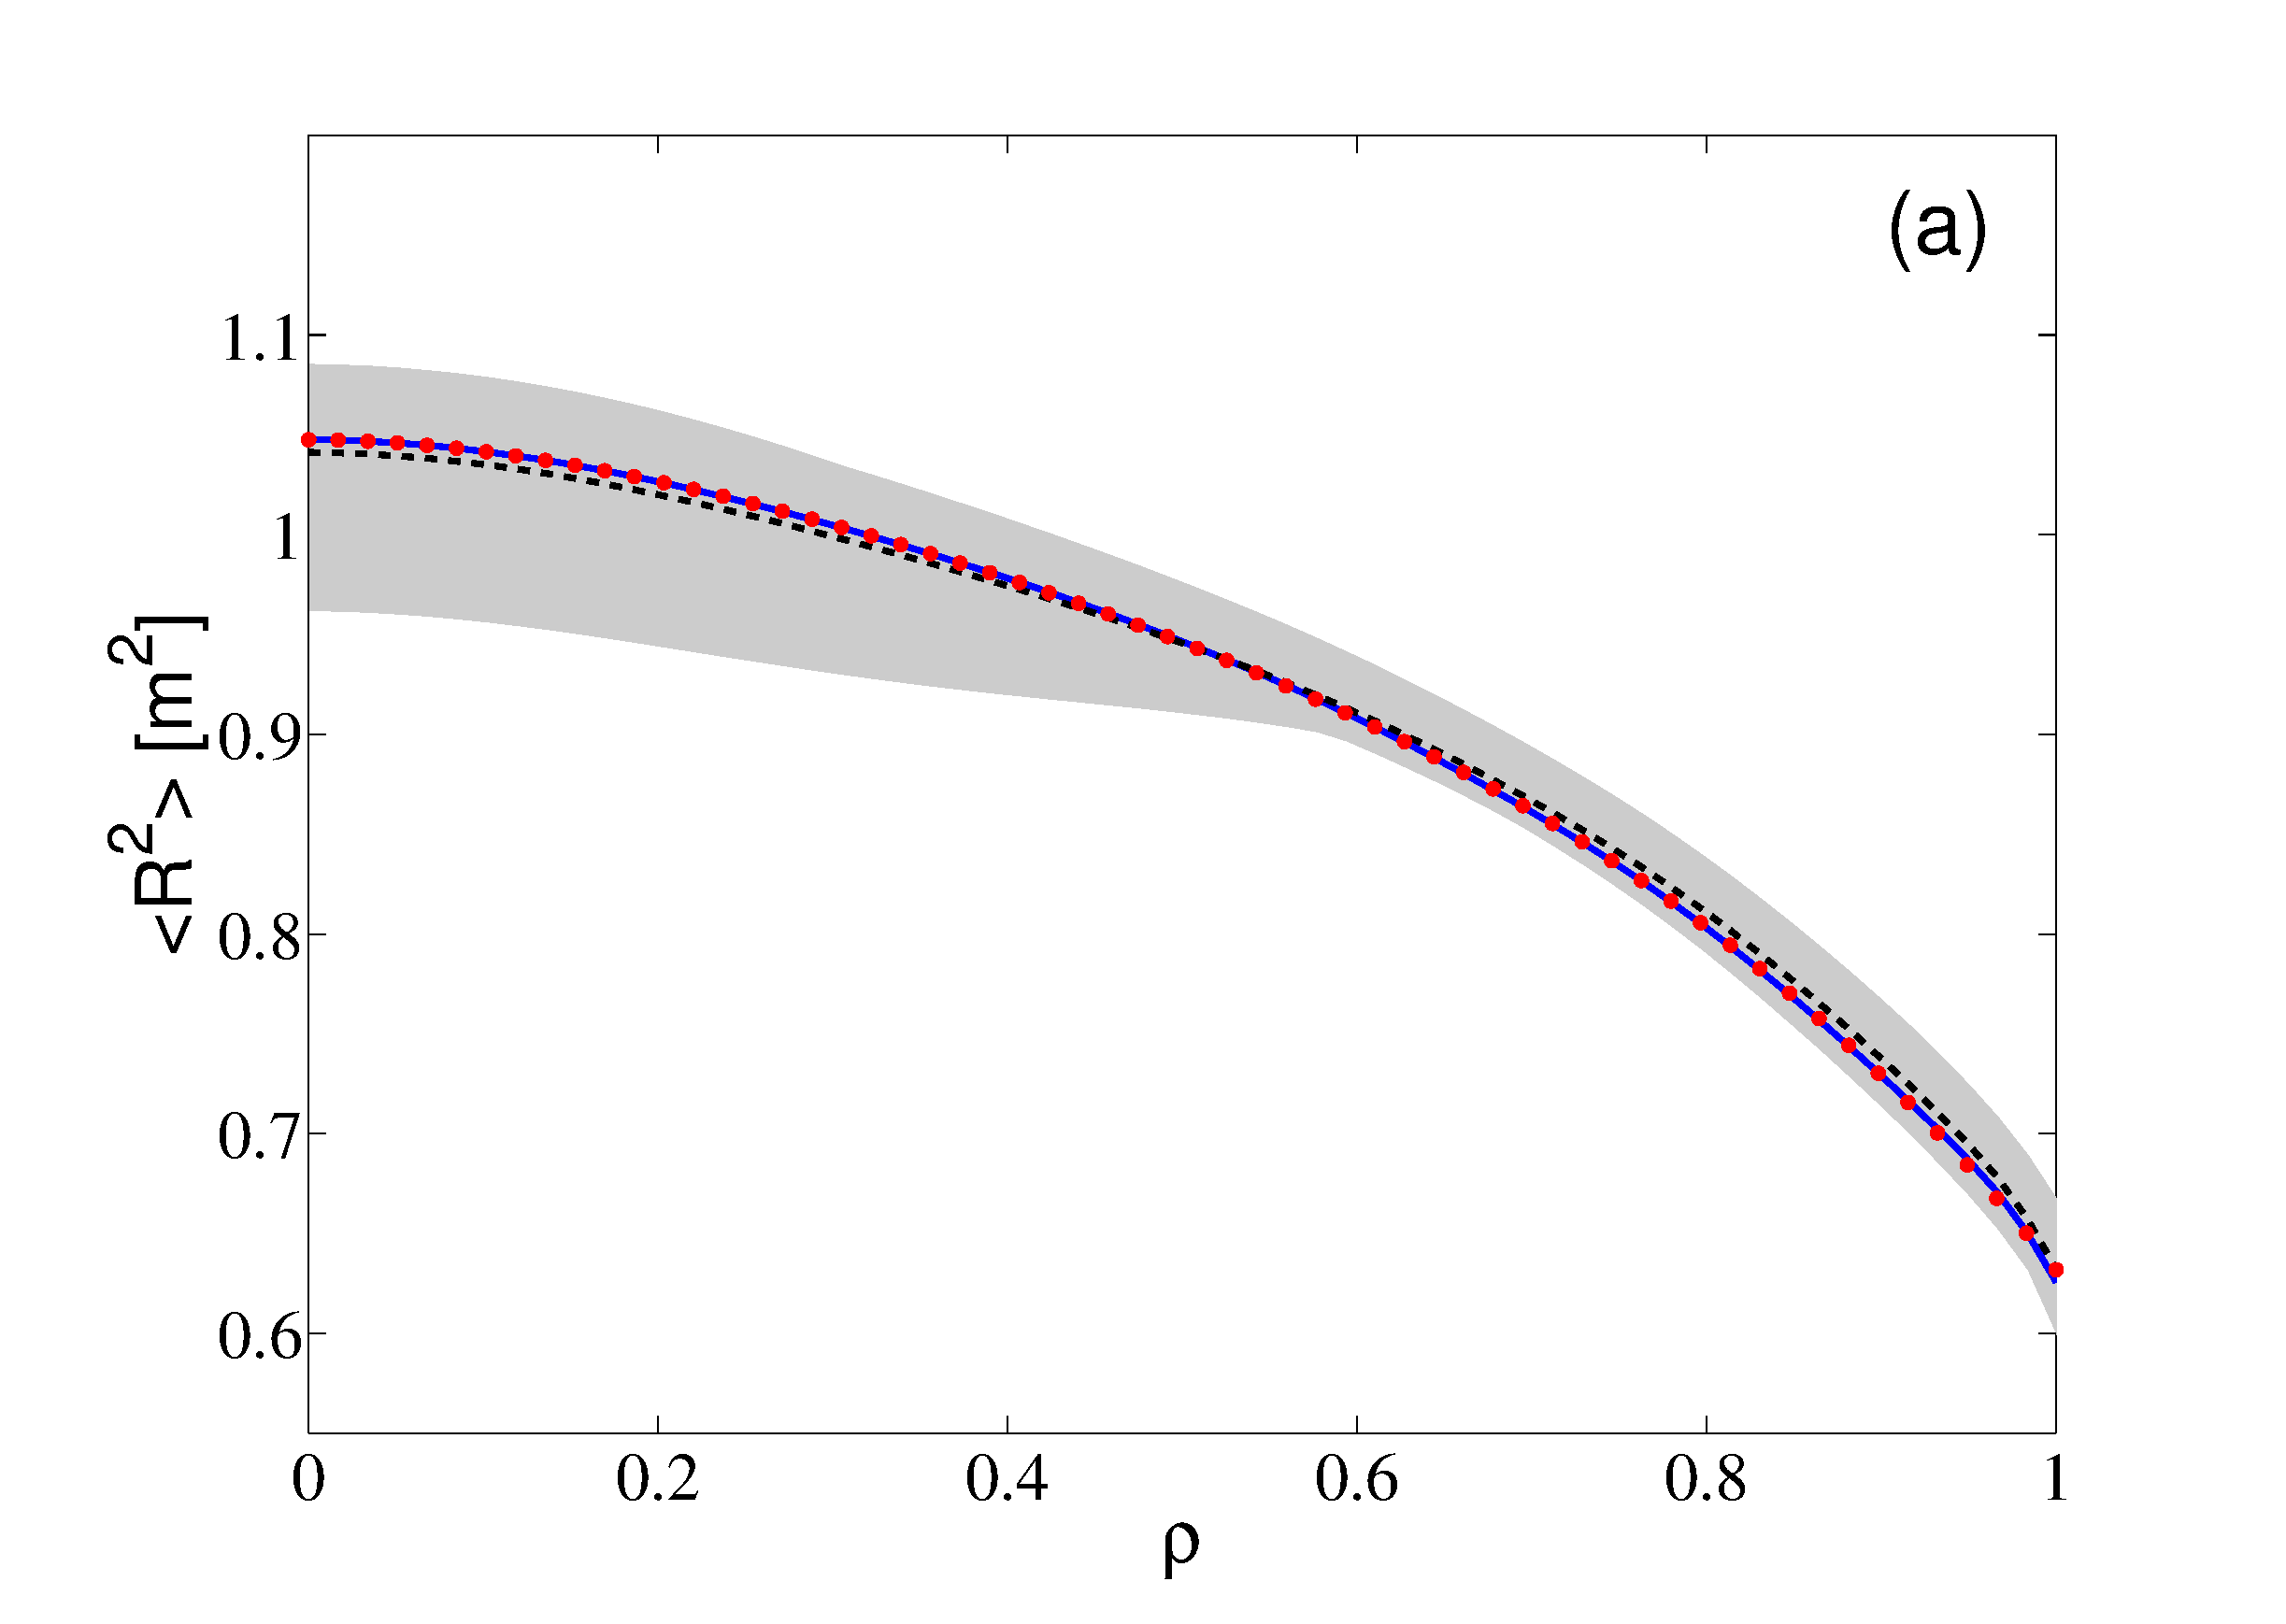
\includegraphics[width=0.5\linewidth]{imene_figs/Goum1} &
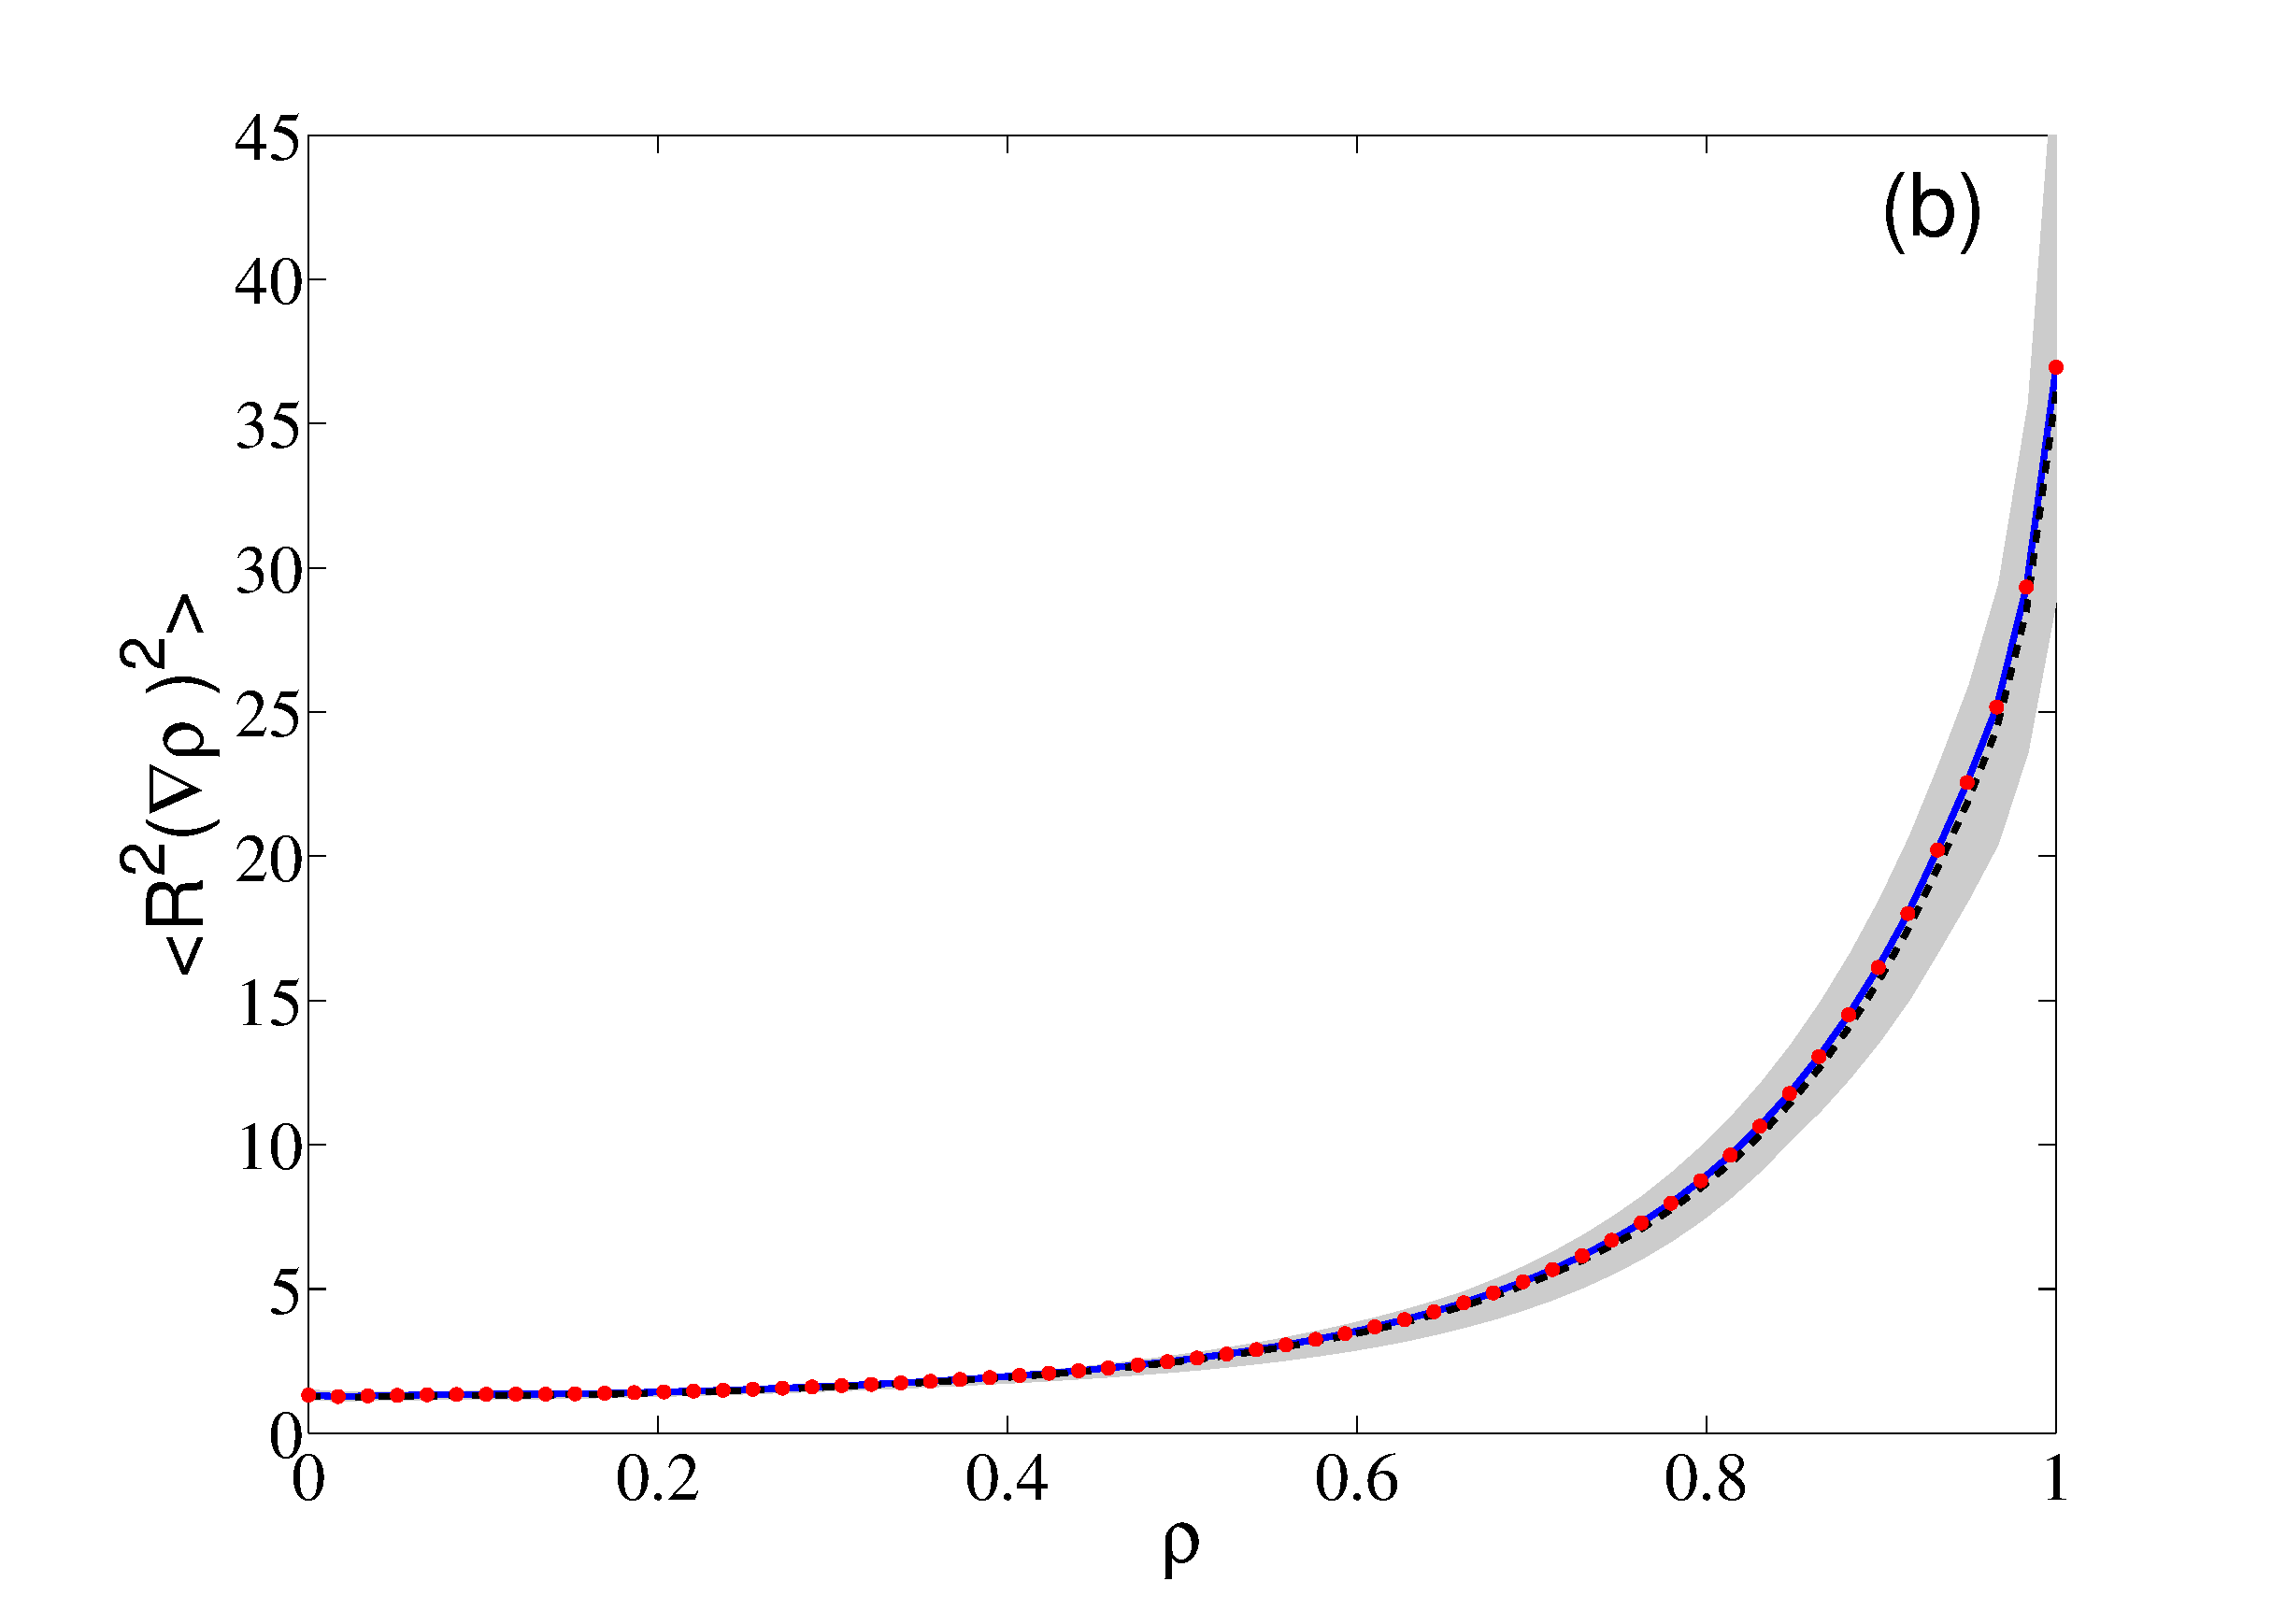
\includegraphics[width= 0.5\linewidth]{imene_figs/Goum2} \\ 
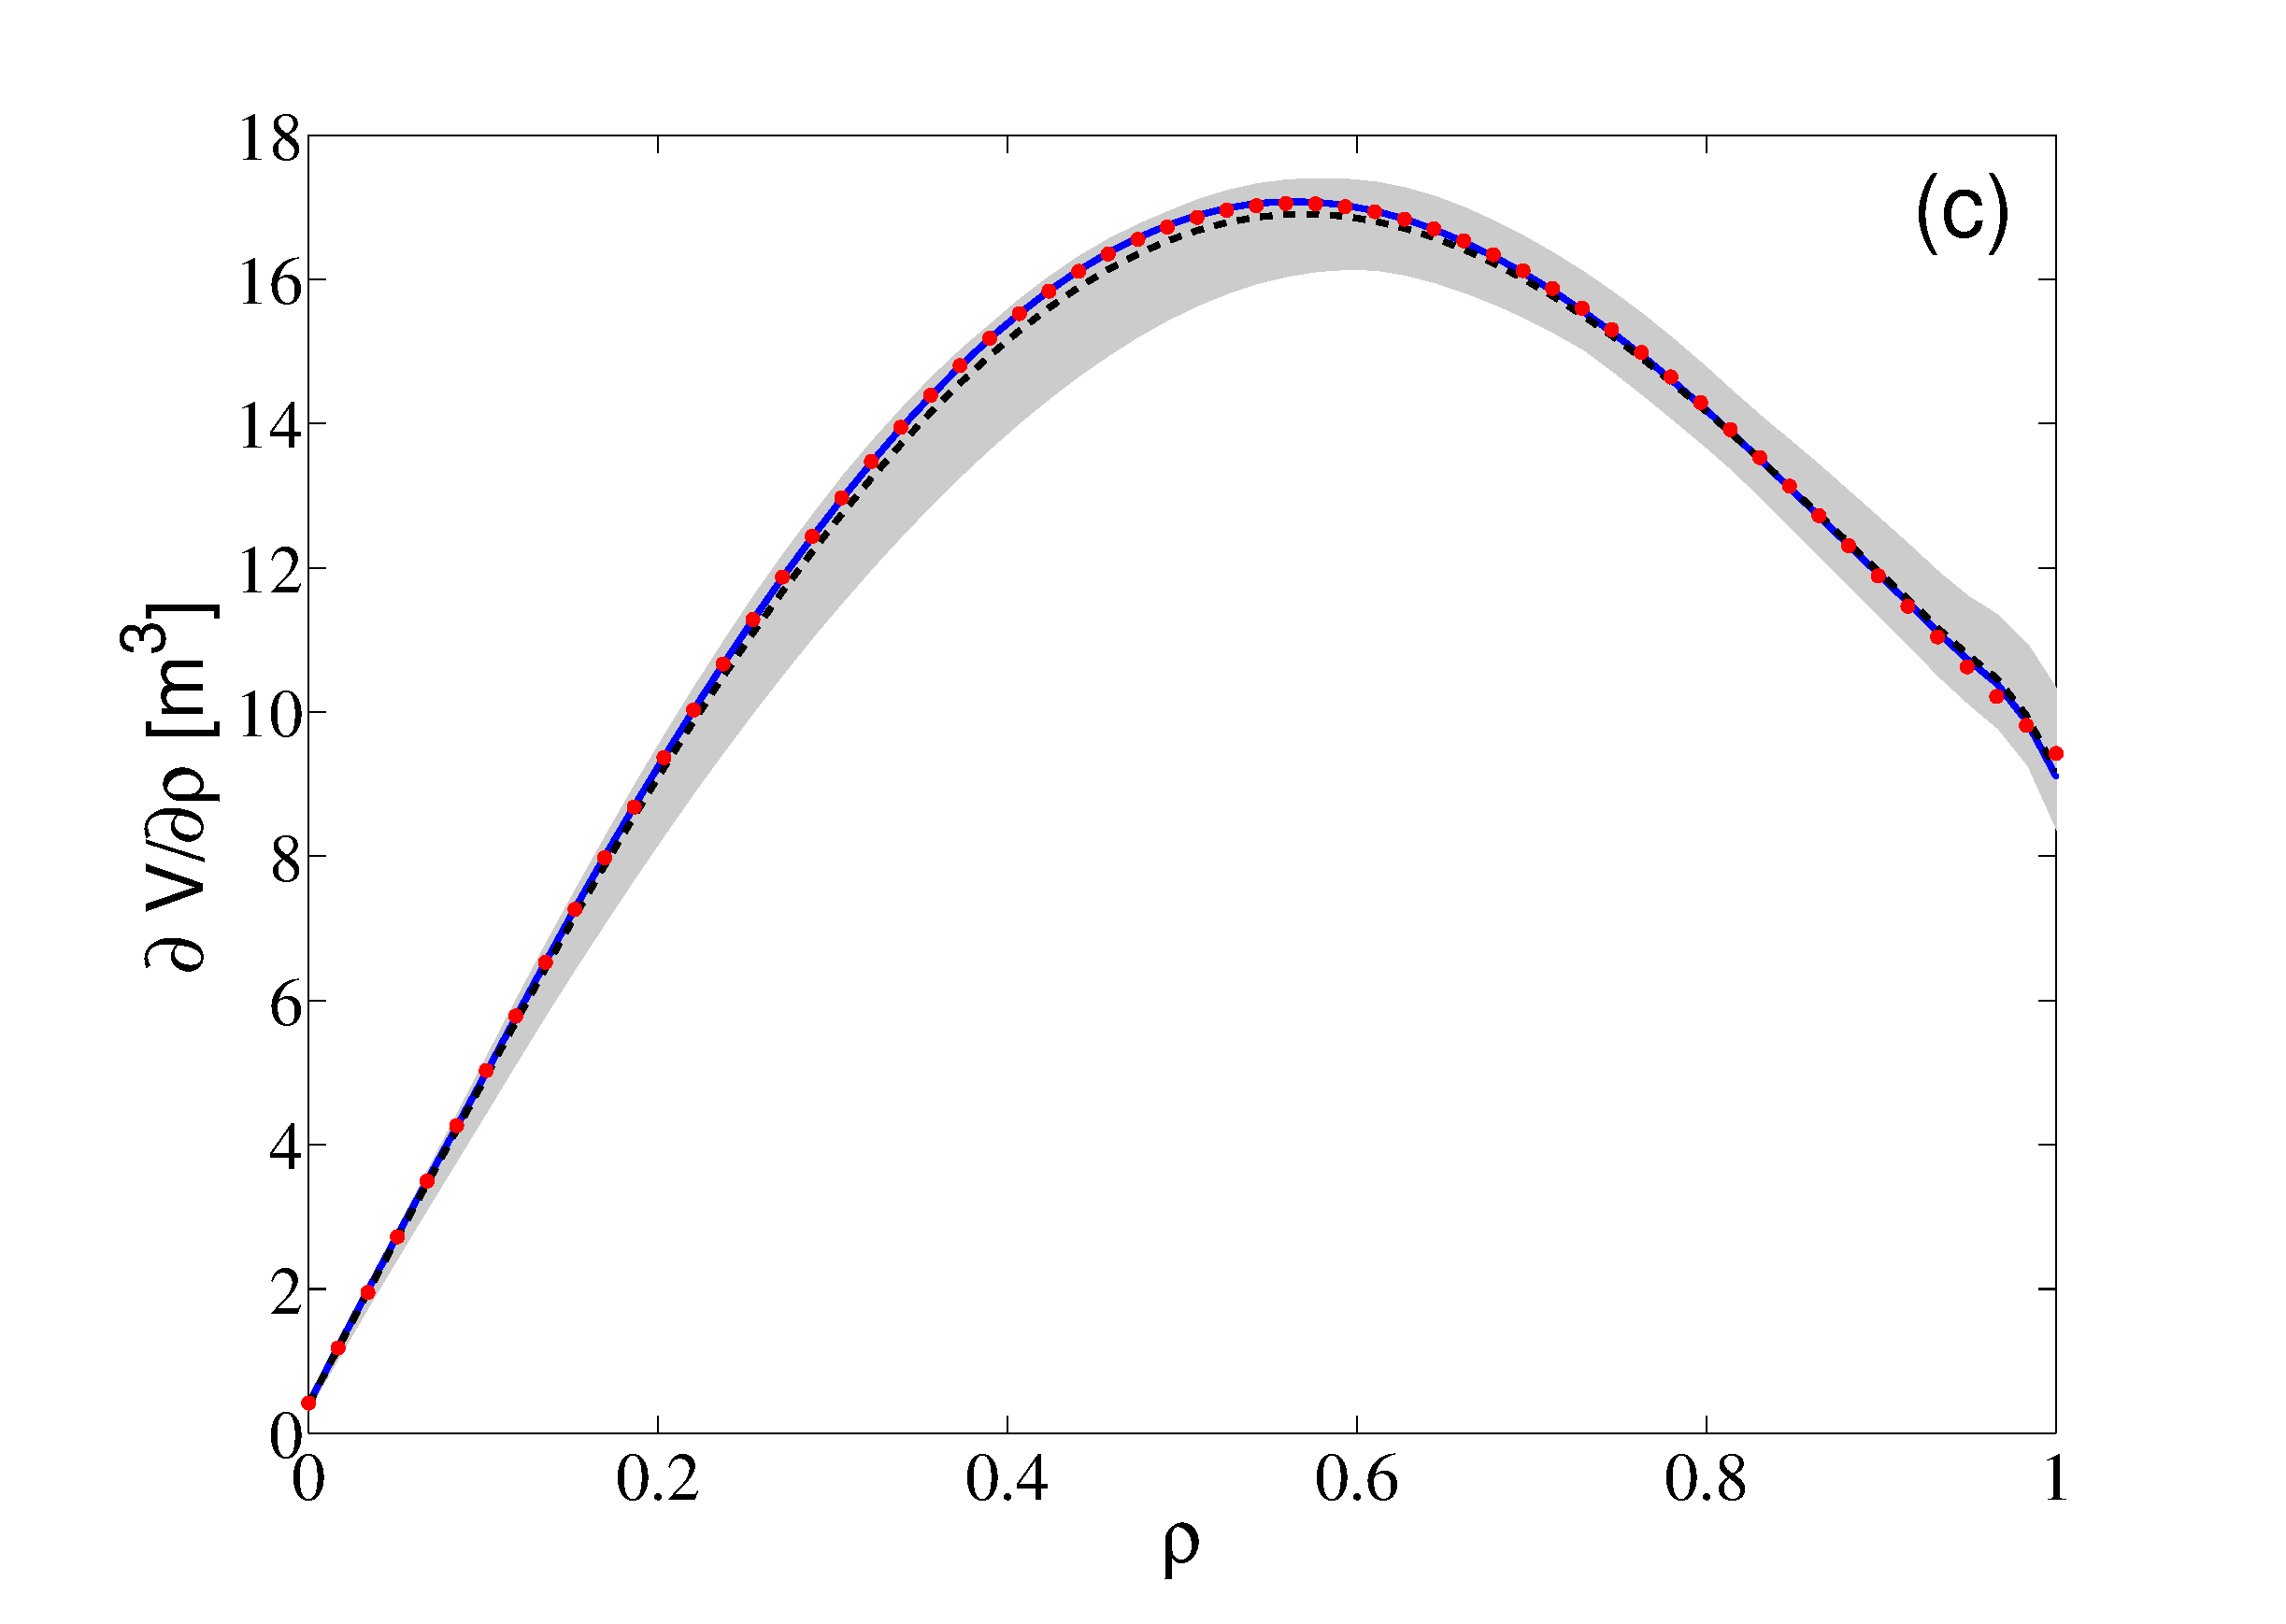
\includegraphics[width=0.5\linewidth]{imene_figs/Goum3} &
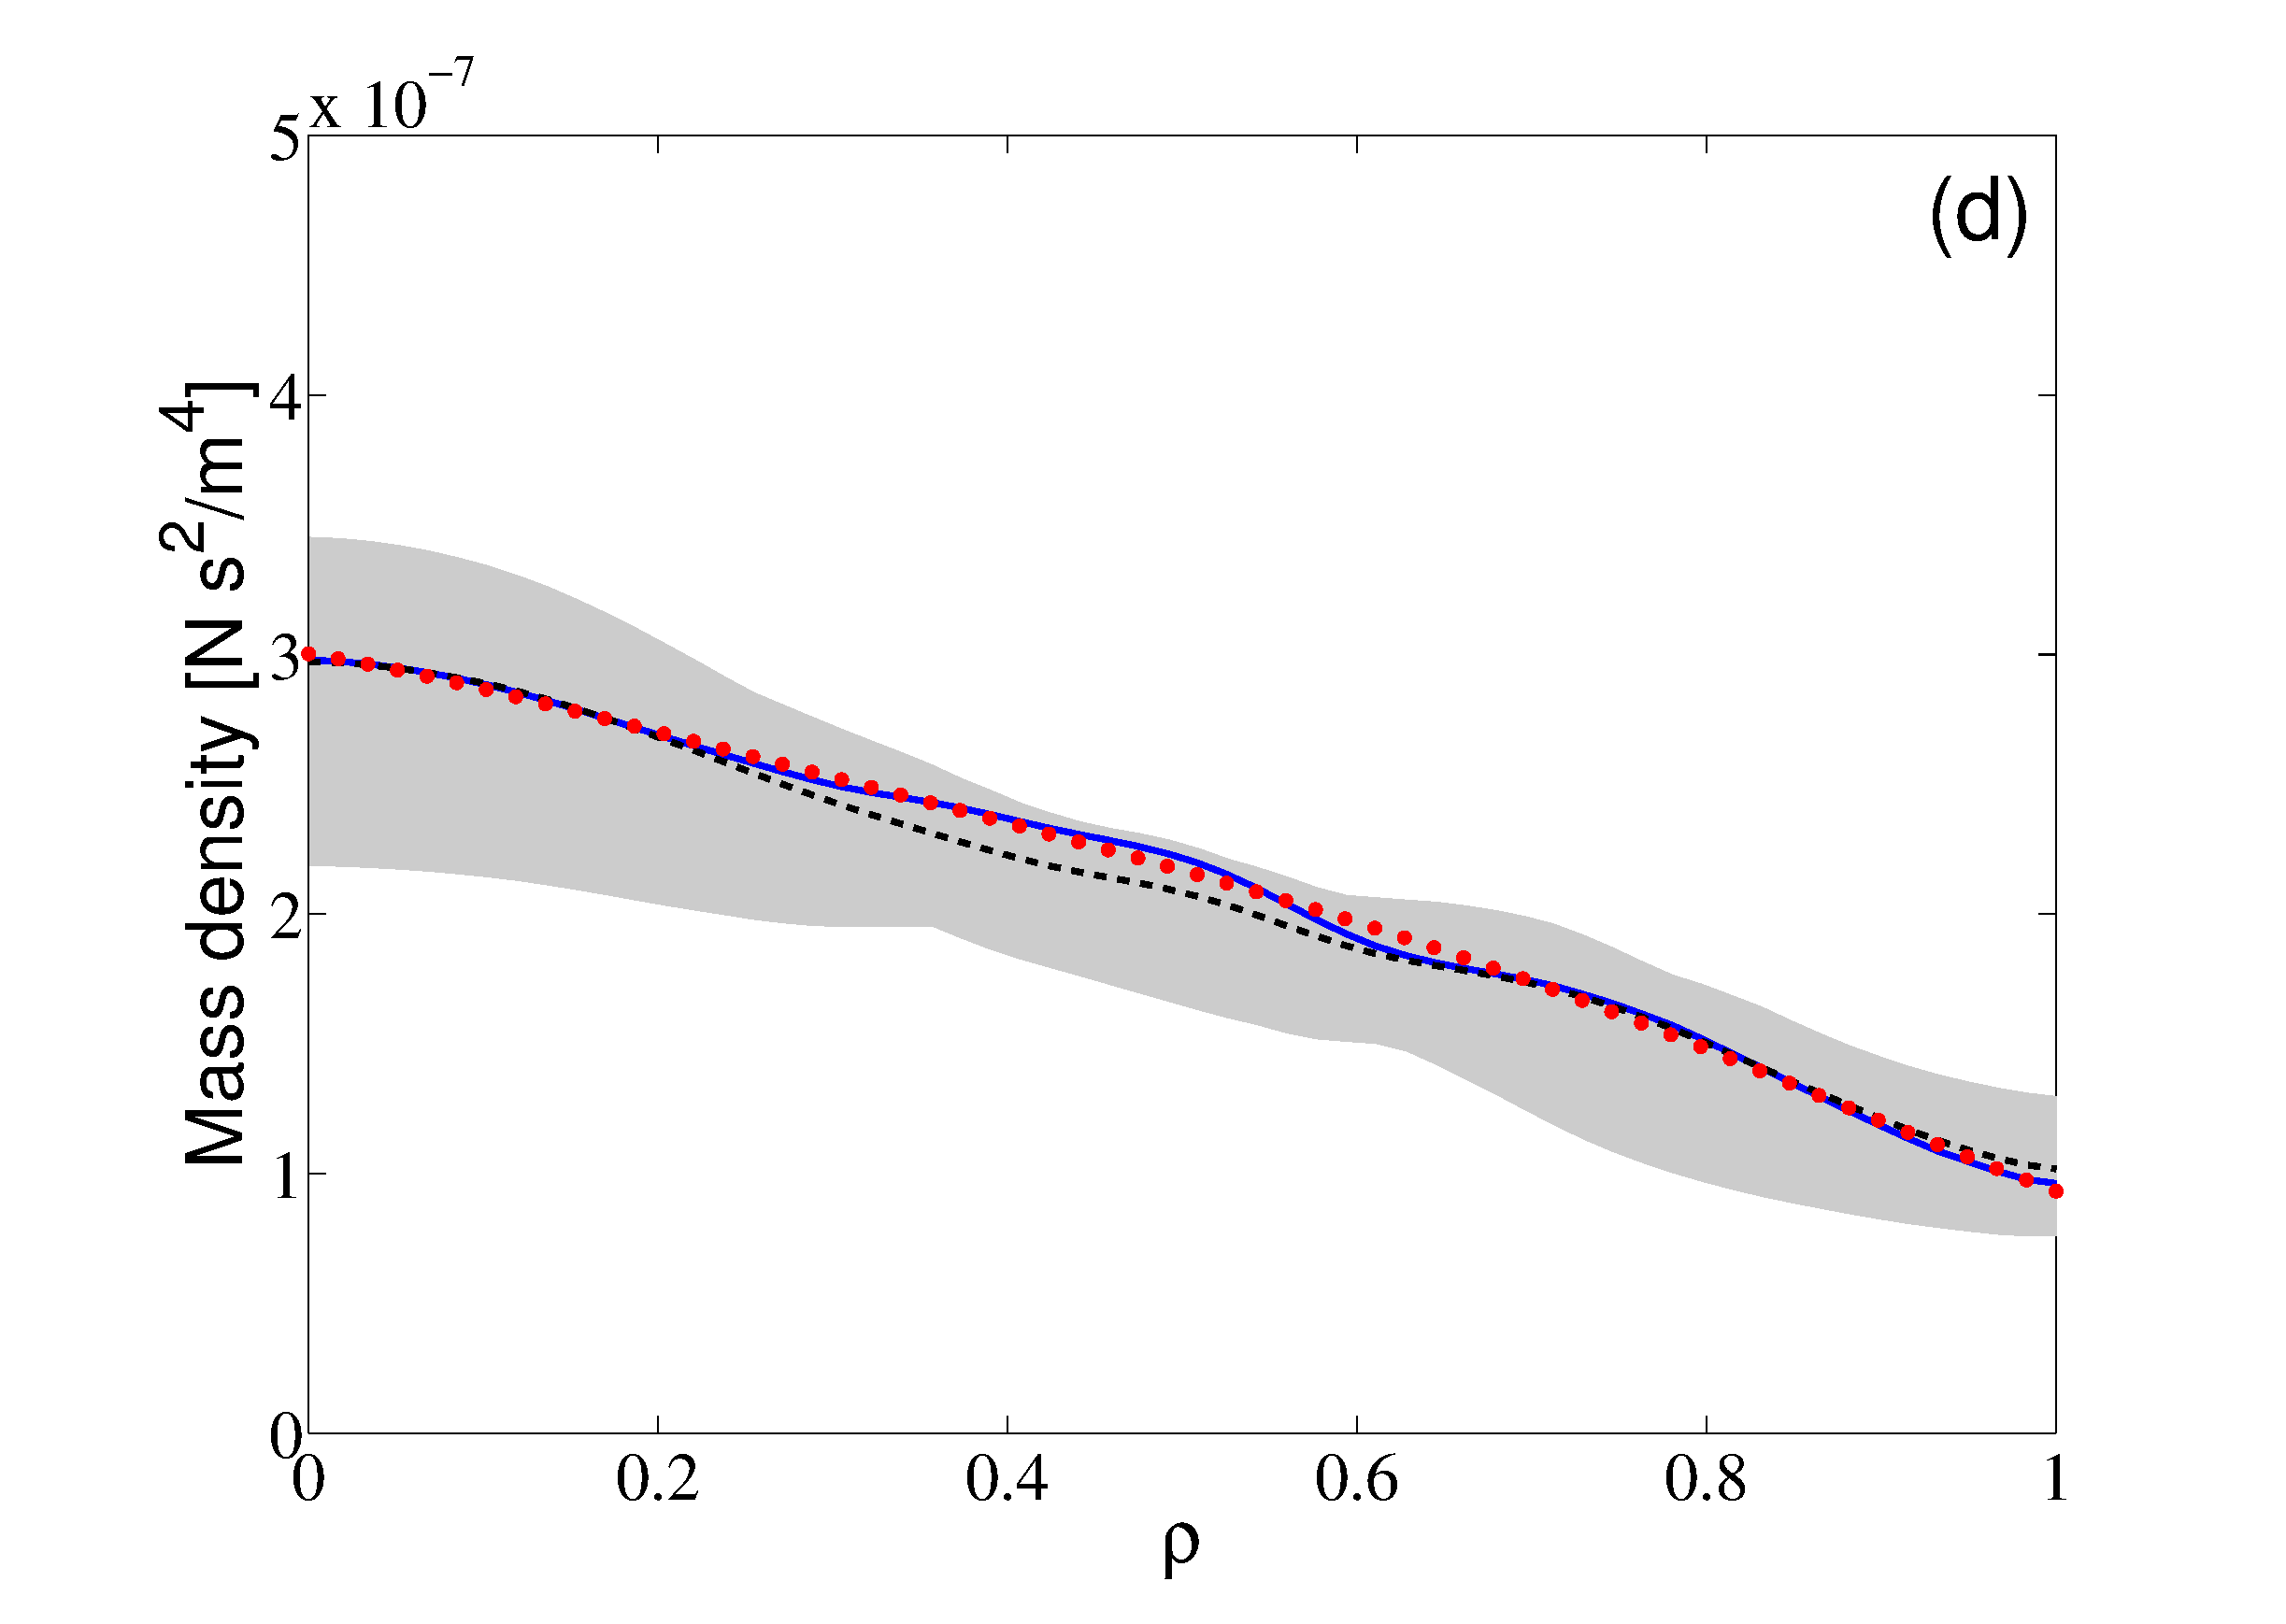
\includegraphics[width=0.5\linewidth]{imene_figs/Goum4} 
\end{tabular}
\caption{Functions describing the shape of the geometrical properties: $\left< R^2 \right>$, $\left< R^2 (\nabla\rho)^2 \right>$, $\partial V/\partial \rho$ and  the mass density $ \sum_i n_i m_i $ from a TRANSP analysis of plasma discharge 133367.  The shaded region represents the value of the function spanned over time interval $(0.45-0.92)$ seconds . The time-average values are shown by the black dashed line (-~-), the frozen time values and its curve-fit are shown by the solid blue lines (-) and the red dots (o) respectively.}
\label{fig:geofunc}
\end{figure}

It is also assumed for simplicity that the time variation of the mass density is small, especially towards the edge, as seen in Figure~{\ref{fig:geofunc}}(\emph{d}). 
 This assumption may latter be removed allowing $ \sum_i n_i m_i $  to vary in time for more complex time dependent systems, but for now, it allows the density time derivative term in the left-hand side of equation~(\ref{eq:full1}) to be neglected resulting in a time invariant system that will be easier to manipulate.
 
 Incorporating these observations into equation~(\ref{eq:full1}), we obtain a more simplified diffusion equation
\begin{eqnarray}
  n m \left<R^2\right>
 \frac{\partial \omega}{\partial t} \nonumber 
 = \left( \frac{\partial V}{\partial\rho}\right)^{-1}
   \frac{\partial}{\partial \rho} 
   \left[\frac{\partial V}{\partial \rho} n m \chi_\phi 
   \left< R^2 (\nabla \rho)^2\right> 
   \frac{\partial\omega}{\partial\rho}\right] 
   + T_\textrm{\tiny NBI} + T_\textrm{\tiny NTV} .
\label{model0}
\end{eqnarray}
$T_\textrm{\tiny NBI} $ and $T_\textrm{\tiny NTV}$ represent the neutral beam injection (NBI) and neoclassical toroidal viscosity (NTV) torques respectively. Note that for this significant class of high confinement discharges, the pinch term and  the momentum loss due to charge exchange are small and the momentum loss due to  field ripple is not required as NTV is explicitly determined in this calculation. Full details of these models are shown in sections~\ref{NBIAM} and \ref{TNTV}.
  
A few observations can be made about this simplified model: First, equation  (\ref{model0}) is parabolic, ensuring the state operator to be negative definite (all eigenvalues are negative);  hence the system is stable, which is a desirable feature from a control viewpoint. 
Second, this approach only models momentum balance for rotation control and does not model potential plasma instabilities.
In fact, this control is meant as an application to avoid plasma instabilities in its future use.
  
The two boundary conditions are chosen consistent with experimental observations to be a symmetry boundary condition at the plasma core and a Dirichelet condition at the edge of the plasma:
\begin{equation}
\left.\frac{\partial\omega}{\partial\rho}\right|_{\rho=0} = 0 
\quad \textrm{and} \quad 
\left.\omega\right|_{\rho=1} = 0.
\label{bc0}
\end{equation}

This data driven model, defined here as a combination of fundamental physics models with quasi static variables fitted to experimental data,  is taken without any temporal dependency on the density  for simplicity, the same is considered for the diffusion coefficient $\chi_\phi$. There are no direct measurements of $\chi_\phi$ inside the tokamak, this quantity has to be reconstructed: during a run of experiments where $\omega$ is measured, TRANSP is able from these measurements to compute an adequately chosen model for  $\chi_\phi$. 

Figure~{\ref{fig:chiphi}} shows the deduced $\chi_\phi$ calculation from a particular run (plasma discharges number 133775). This run is identical to the plasma discharge number 133367 except that it does not have an applied non-axisymmetric field, and therefore $T_\textrm{\tiny NTV} = 0$. This feature is very important because each dissipation effect needs to be considered separately from each source in the model. Therefore, the data driven model will use the $\chi_\phi$ of this former plasma discharge (133775) as its momentum diffusivity coefficient reference.


\begin{figure}
\centering
\begin{tabular}{c}
Shot no 133775 \\
 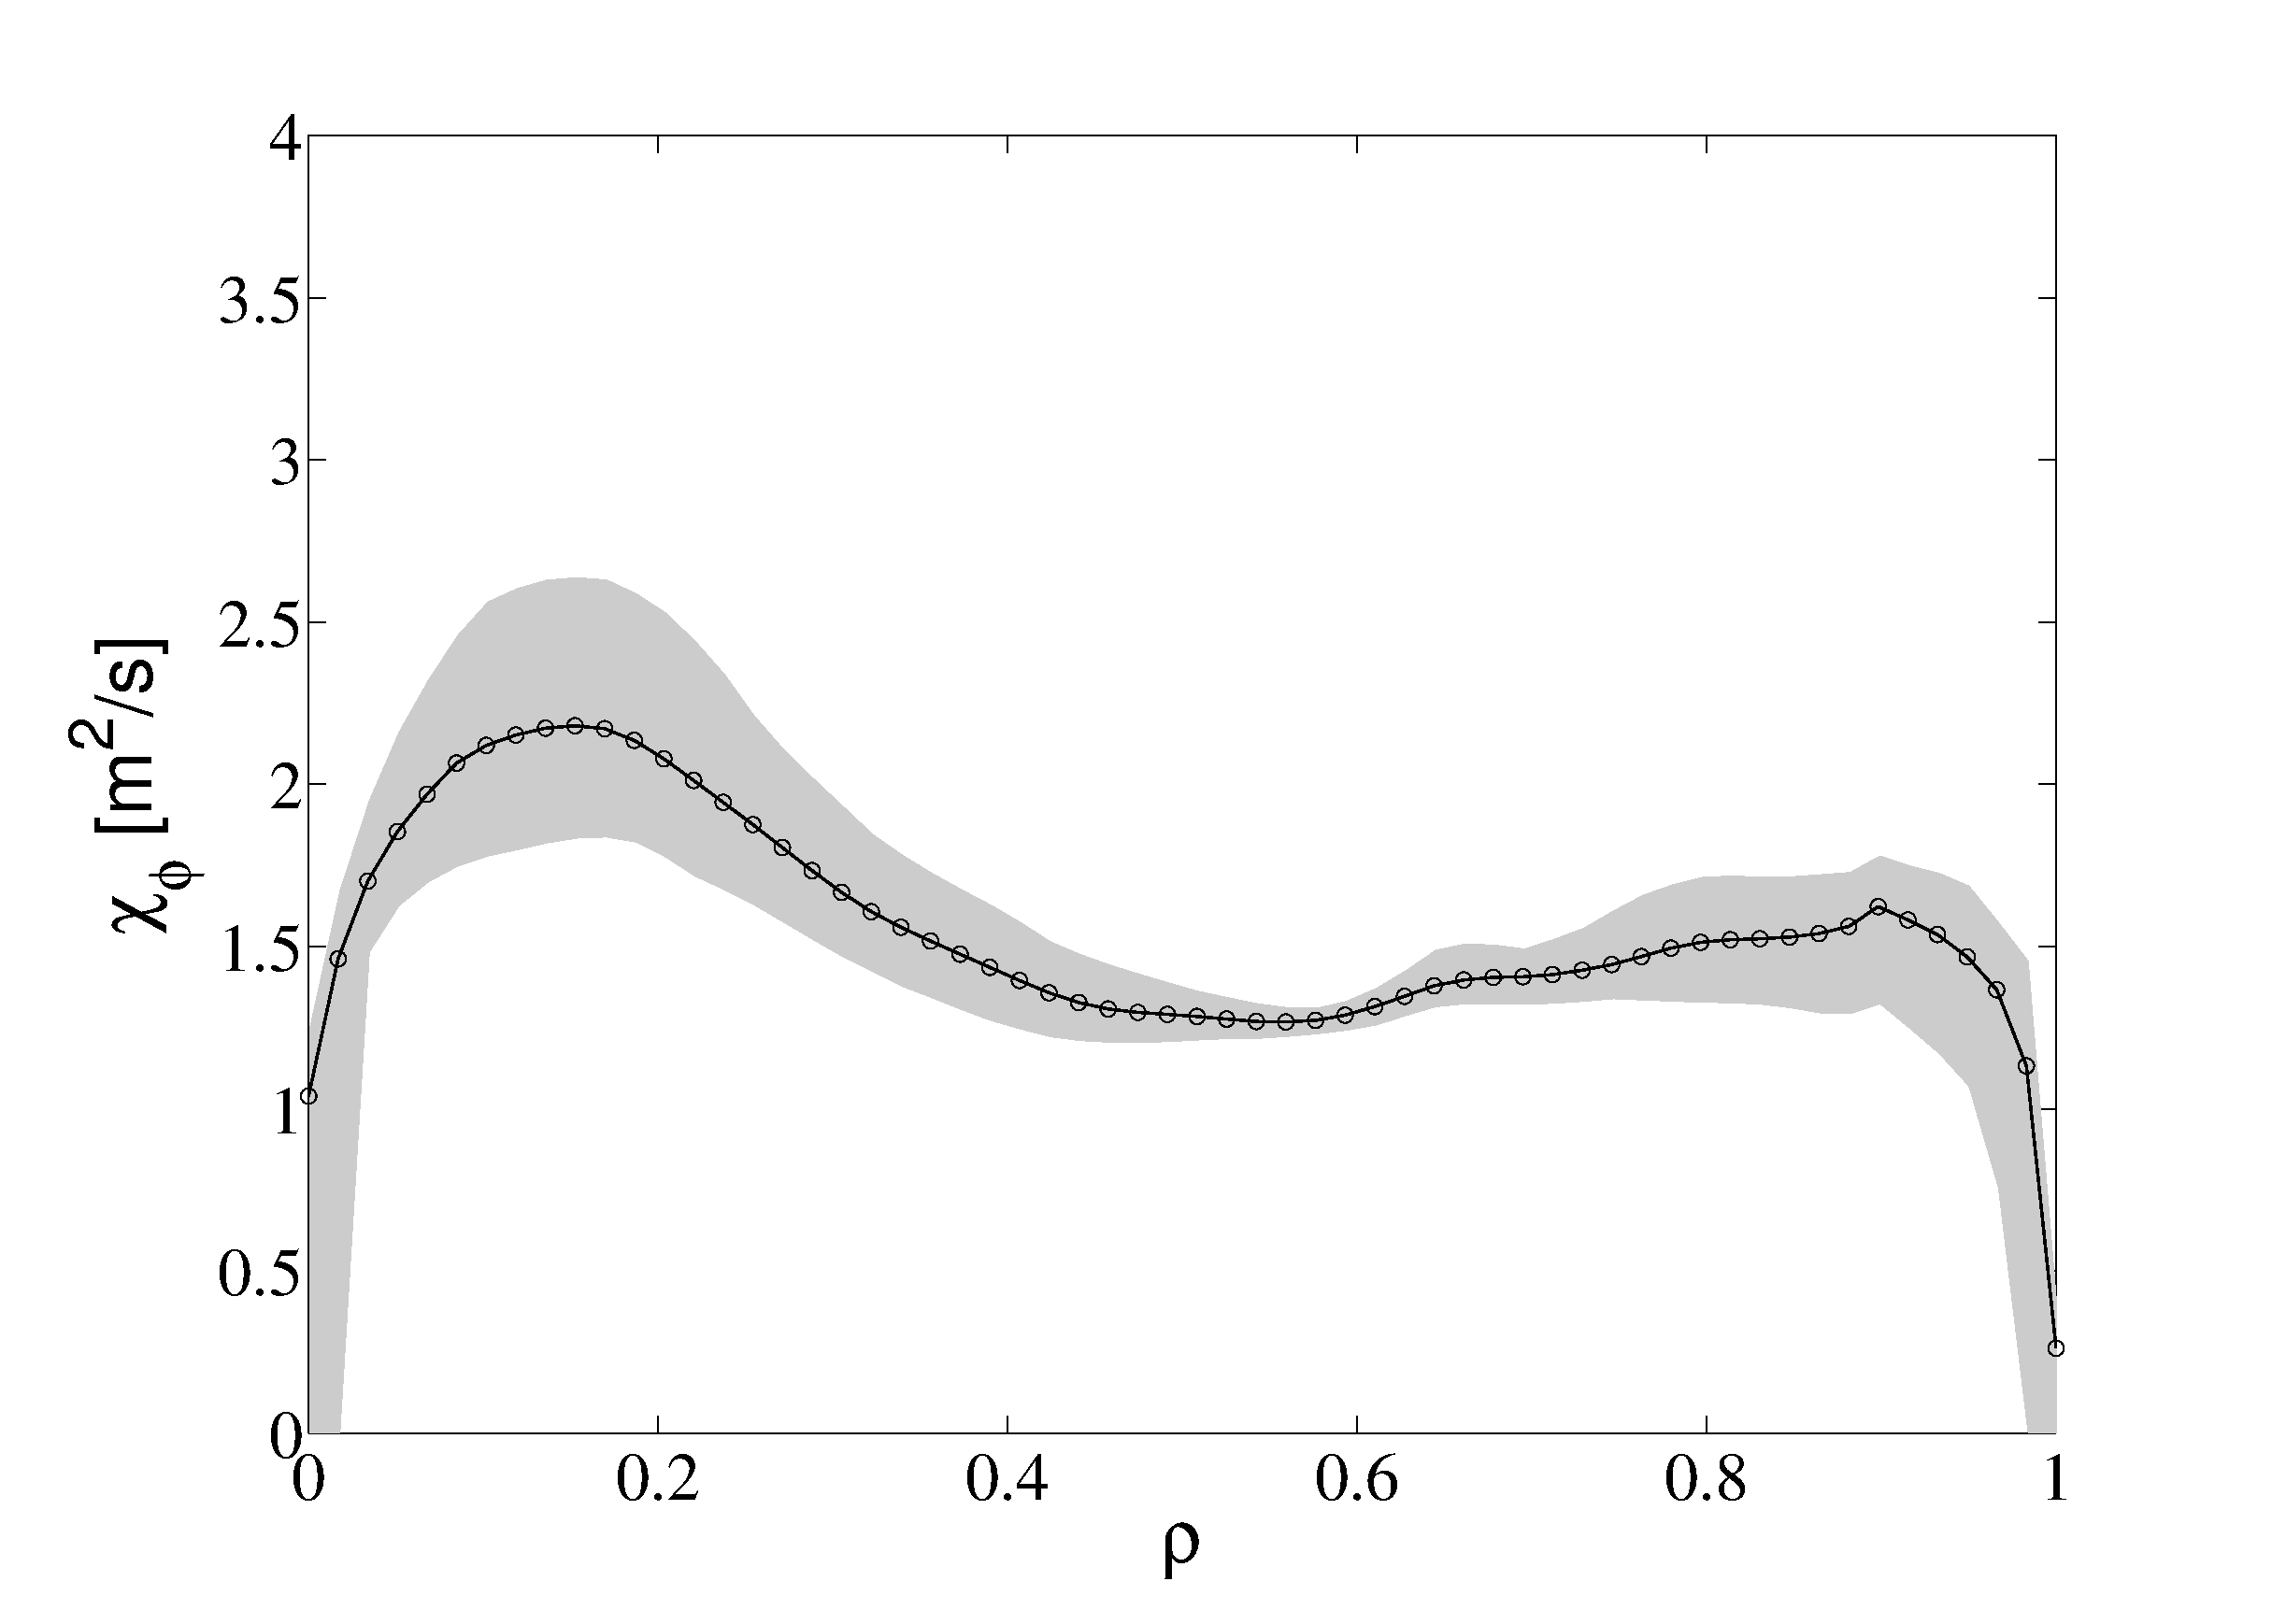
\includegraphics[width=\linewidth]{imene_figs/CHIPHI1n}
 \end{tabular}
\caption{The momentum diffusivity coefficient $ \chi_{\phi}$ is calculated through TRANSP analysis. The time-average values and their curve-fits are shown by the circles  and the solid lines respectively}
\label{fig:chiphi}
\end{figure}


The approach here is: given a desired plasma rotation profile that the operator wishes the system to reach and stabilize around, take the simplified model (equation~\ref{model0}) that relies on different models of $ n  m$, NTV and NBI torques from a representative class of plasma discharge ($\chi_\phi$ modeled from plasma discharge 133775), and use it to design a controller that will attempt to match any desired profile shape.

\subsection{Actuators models}

In order to control the toroidal momentum of the plasma in a spherical tokamak, we consider the use of two actuator mechanisms, namely, the neutral beam injection (NBI) and the neoclassical toroidal viscosity (NTV). The neutral beams are the main sources of momentum for the plasma and the NTV actuator is primarily used as a source of drag on the plasma. For NSTX, $T_\textrm{\tiny NBI}$ is strongest  in the plasma core, whereas $T_\textrm{\tiny NTV}$ is strongest further out in the plasma. The momentum diffusivity $\chi_\phi$ allows transport of the momentum across these plasma regimes on the momentum diffusion timescale of about $0.1\,s$ in NSTX H-mode plasmas.


\subsubsection{Neutral Beam Injection (NBI) actuator model}
 \label{NBIAM}

In NSTX, neutral beam injection is the main method to produce positive torque to increase plasma rotation, which is achieved  by injecting high-speed neutral atoms into the center of the plasma. Figure~{\ref{NBI_pics}} shows the planned neutral beam injection for the present upgrade of NSTX. In the present study, we consider the three neutral beam sources injected from the injector shown on the left of the figure.
 Neutral atoms are able to cross the confining magnetic field of the tokamak without being deflected, and are ionized in the plasma via collisions with ions and electrons. The fast ions that are generated are also confined in the magnetic field and are able to exchange their energy to plasma ions and electrons. Typical injection acceleration voltages are in the range of 50\,keV to 130\,keV and for comparison, in NSTX, the peak plasma ion thermal temperature reaches up to $1.5$ keV.

\begin{figure}
\begin{tabular}{cc}
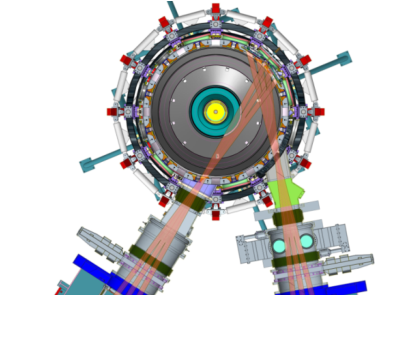
\includegraphics[width=0.5\linewidth]{imene_figs/pic_NBI1} &
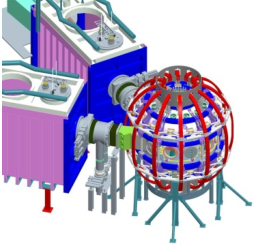
\includegraphics[width=0.4\linewidth]{imene_figs/pic_NBI2}
\end{tabular}
\caption{Illustration of the neutral beam injection (NBI) devices for NSTX-U with an inside view from the top of the tokamak (left) and outside view (right). }
\label{NBI_pics}
\end{figure}


A differential-equation model is introduced to relate the input power to the generated torque.  First, we start by writing the NBI torque as a product of the spatial average of the torque, $\overline{T}_\textrm{\tiny{NBI}}(t) \equiv \textrm{avg}_\rho T_\textrm{\tiny{NBI}}(t,\rho)$, and a function, $F_\textrm{\tiny{NBI}}(\rho)$, that represents the spatial profile
\begin{equation}
   T_\textrm{\tiny{NBI}}(t,\rho) = \overline{T}_\textrm{\tiny{NBI}}(t) F_\textrm{\tiny{NBI}}(\rho),
\label{eq5}
\end{equation}
where the spatial profile of the torque is taken to be a Gaussian function (based on TRANSP analysis of NSTX discharge 133367) written as
\begin{equation}
F_\textrm{\tiny{NBI}}(\rho) = a_\textrm{\tiny{NBI}} \exp\left( - \frac{\rho^2}{2\sigma^2\textrm{\tiny{NBI}}}\right).
\label{eq6}
\end{equation}

\begin{figure}
\begin{tabular}{cc}
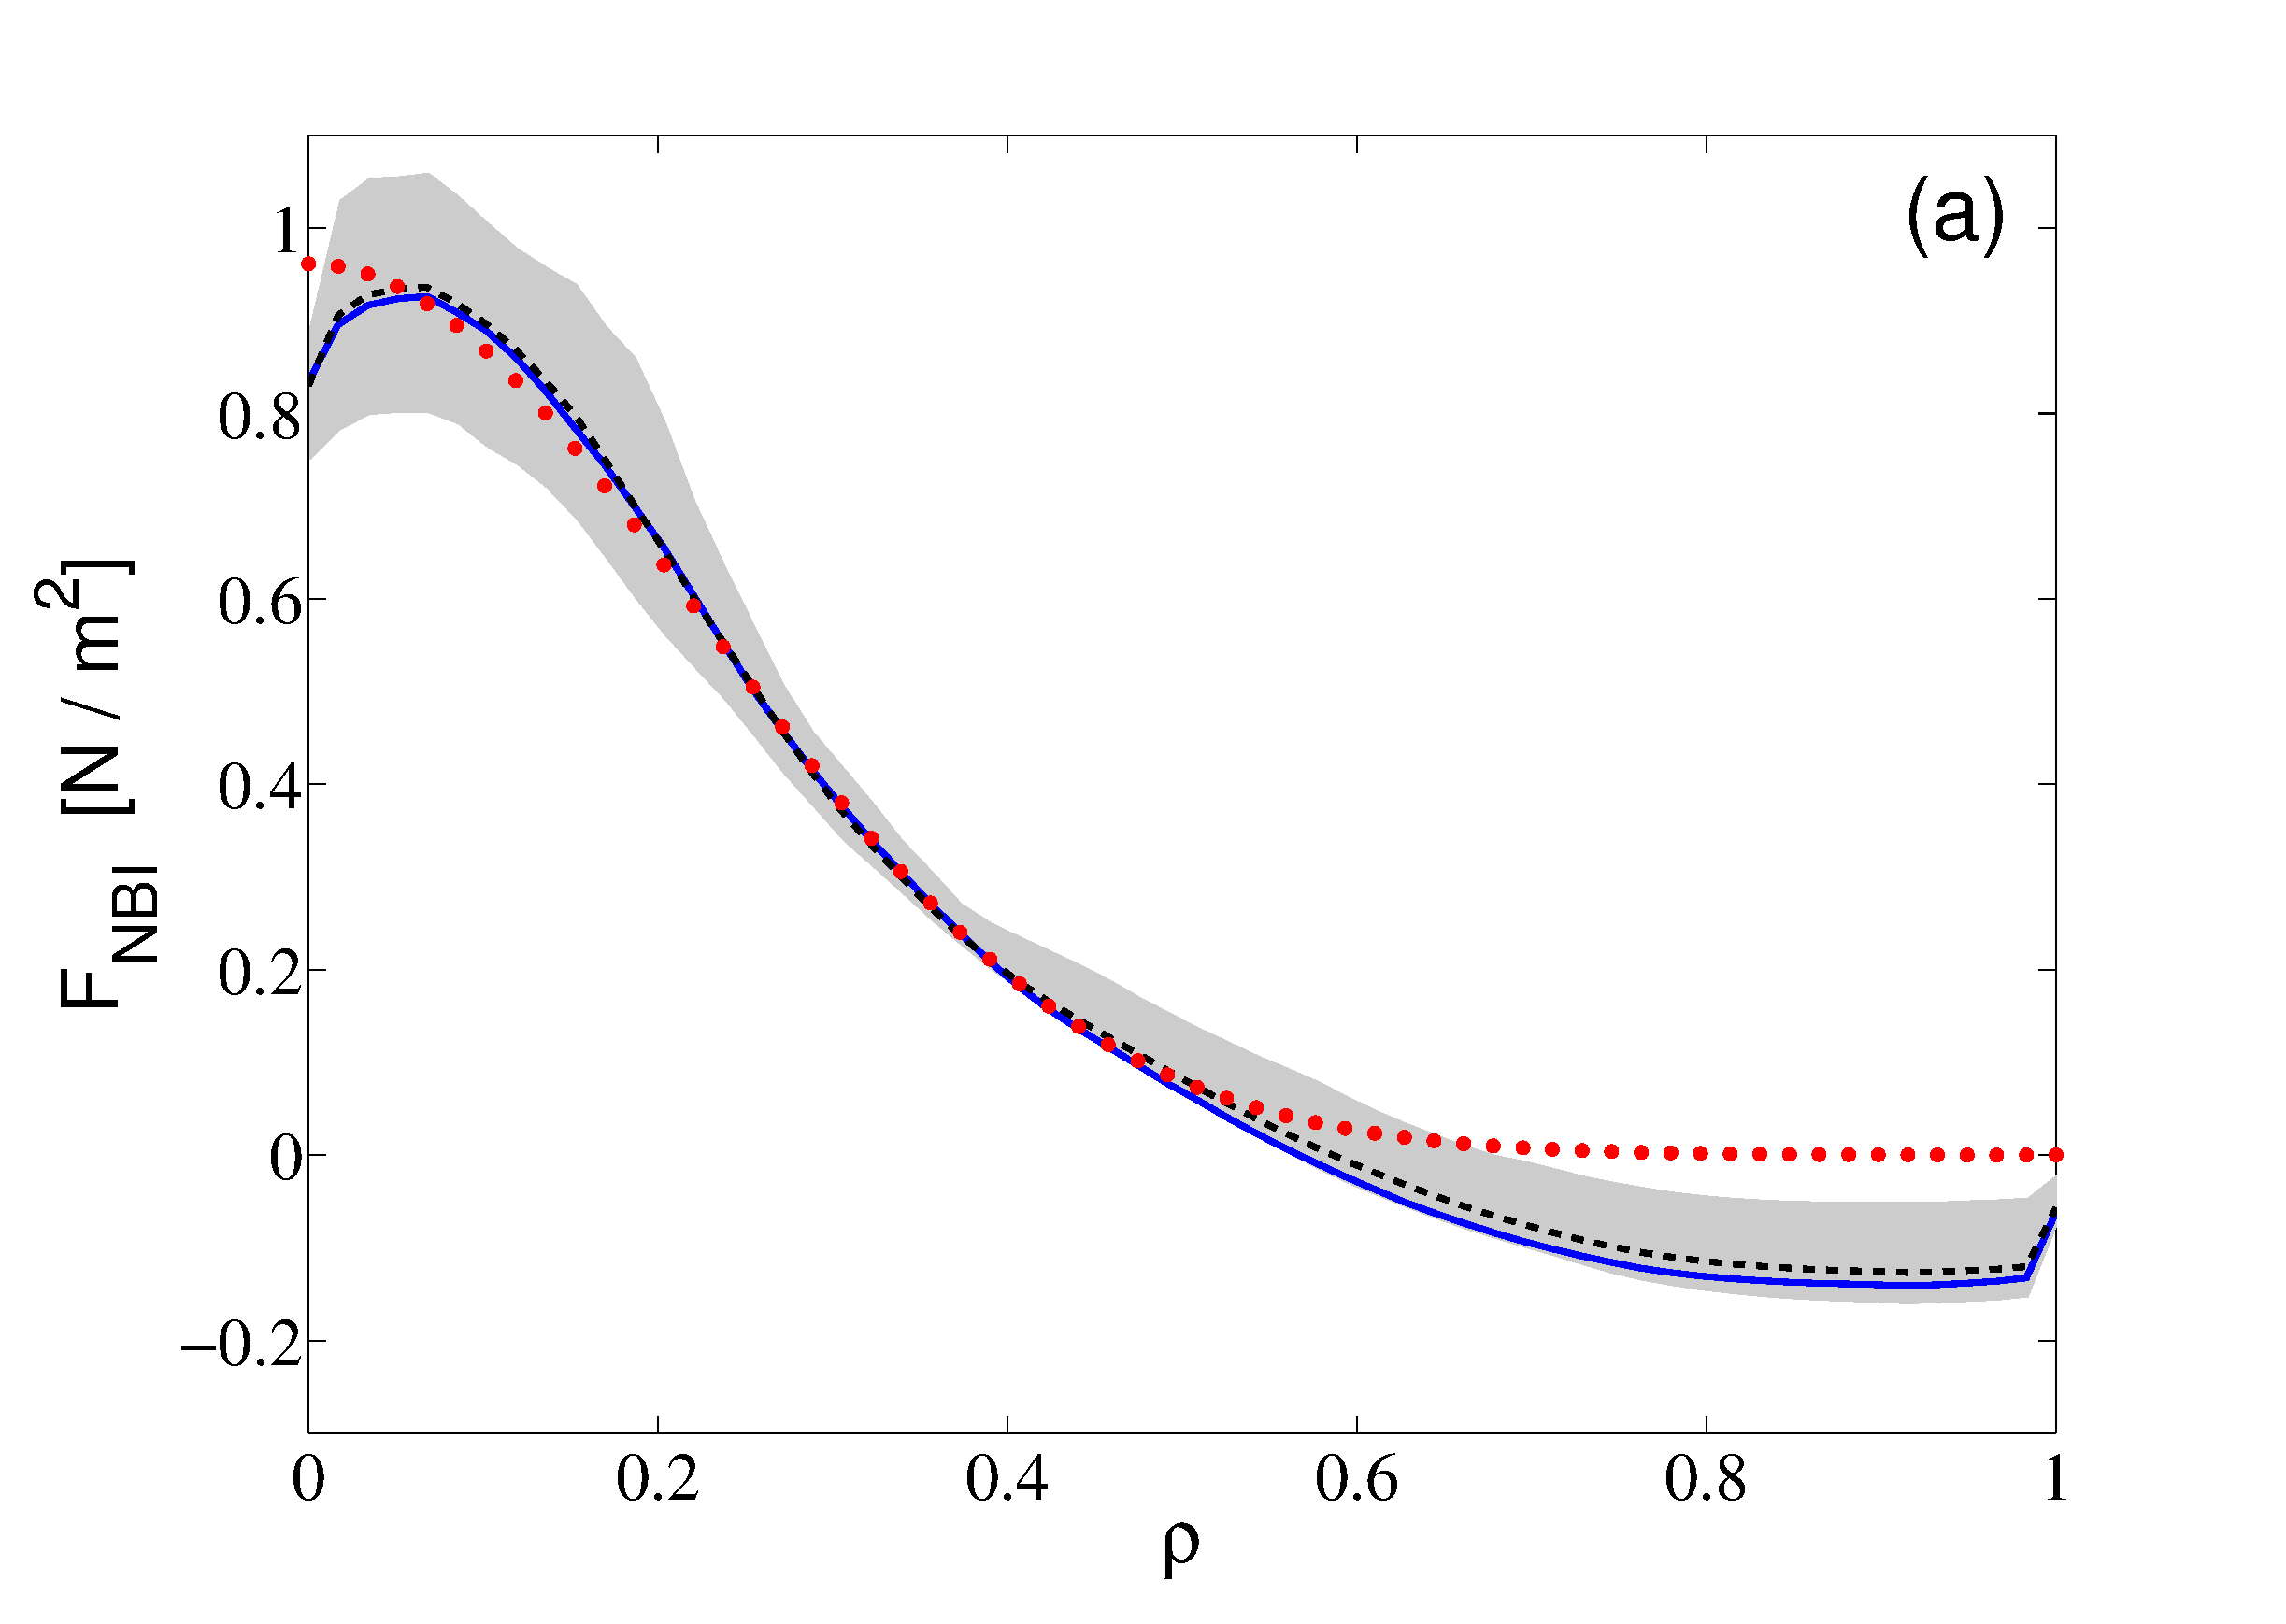
\includegraphics[width=0.5\linewidth]{imene_figs/Goum7}& 
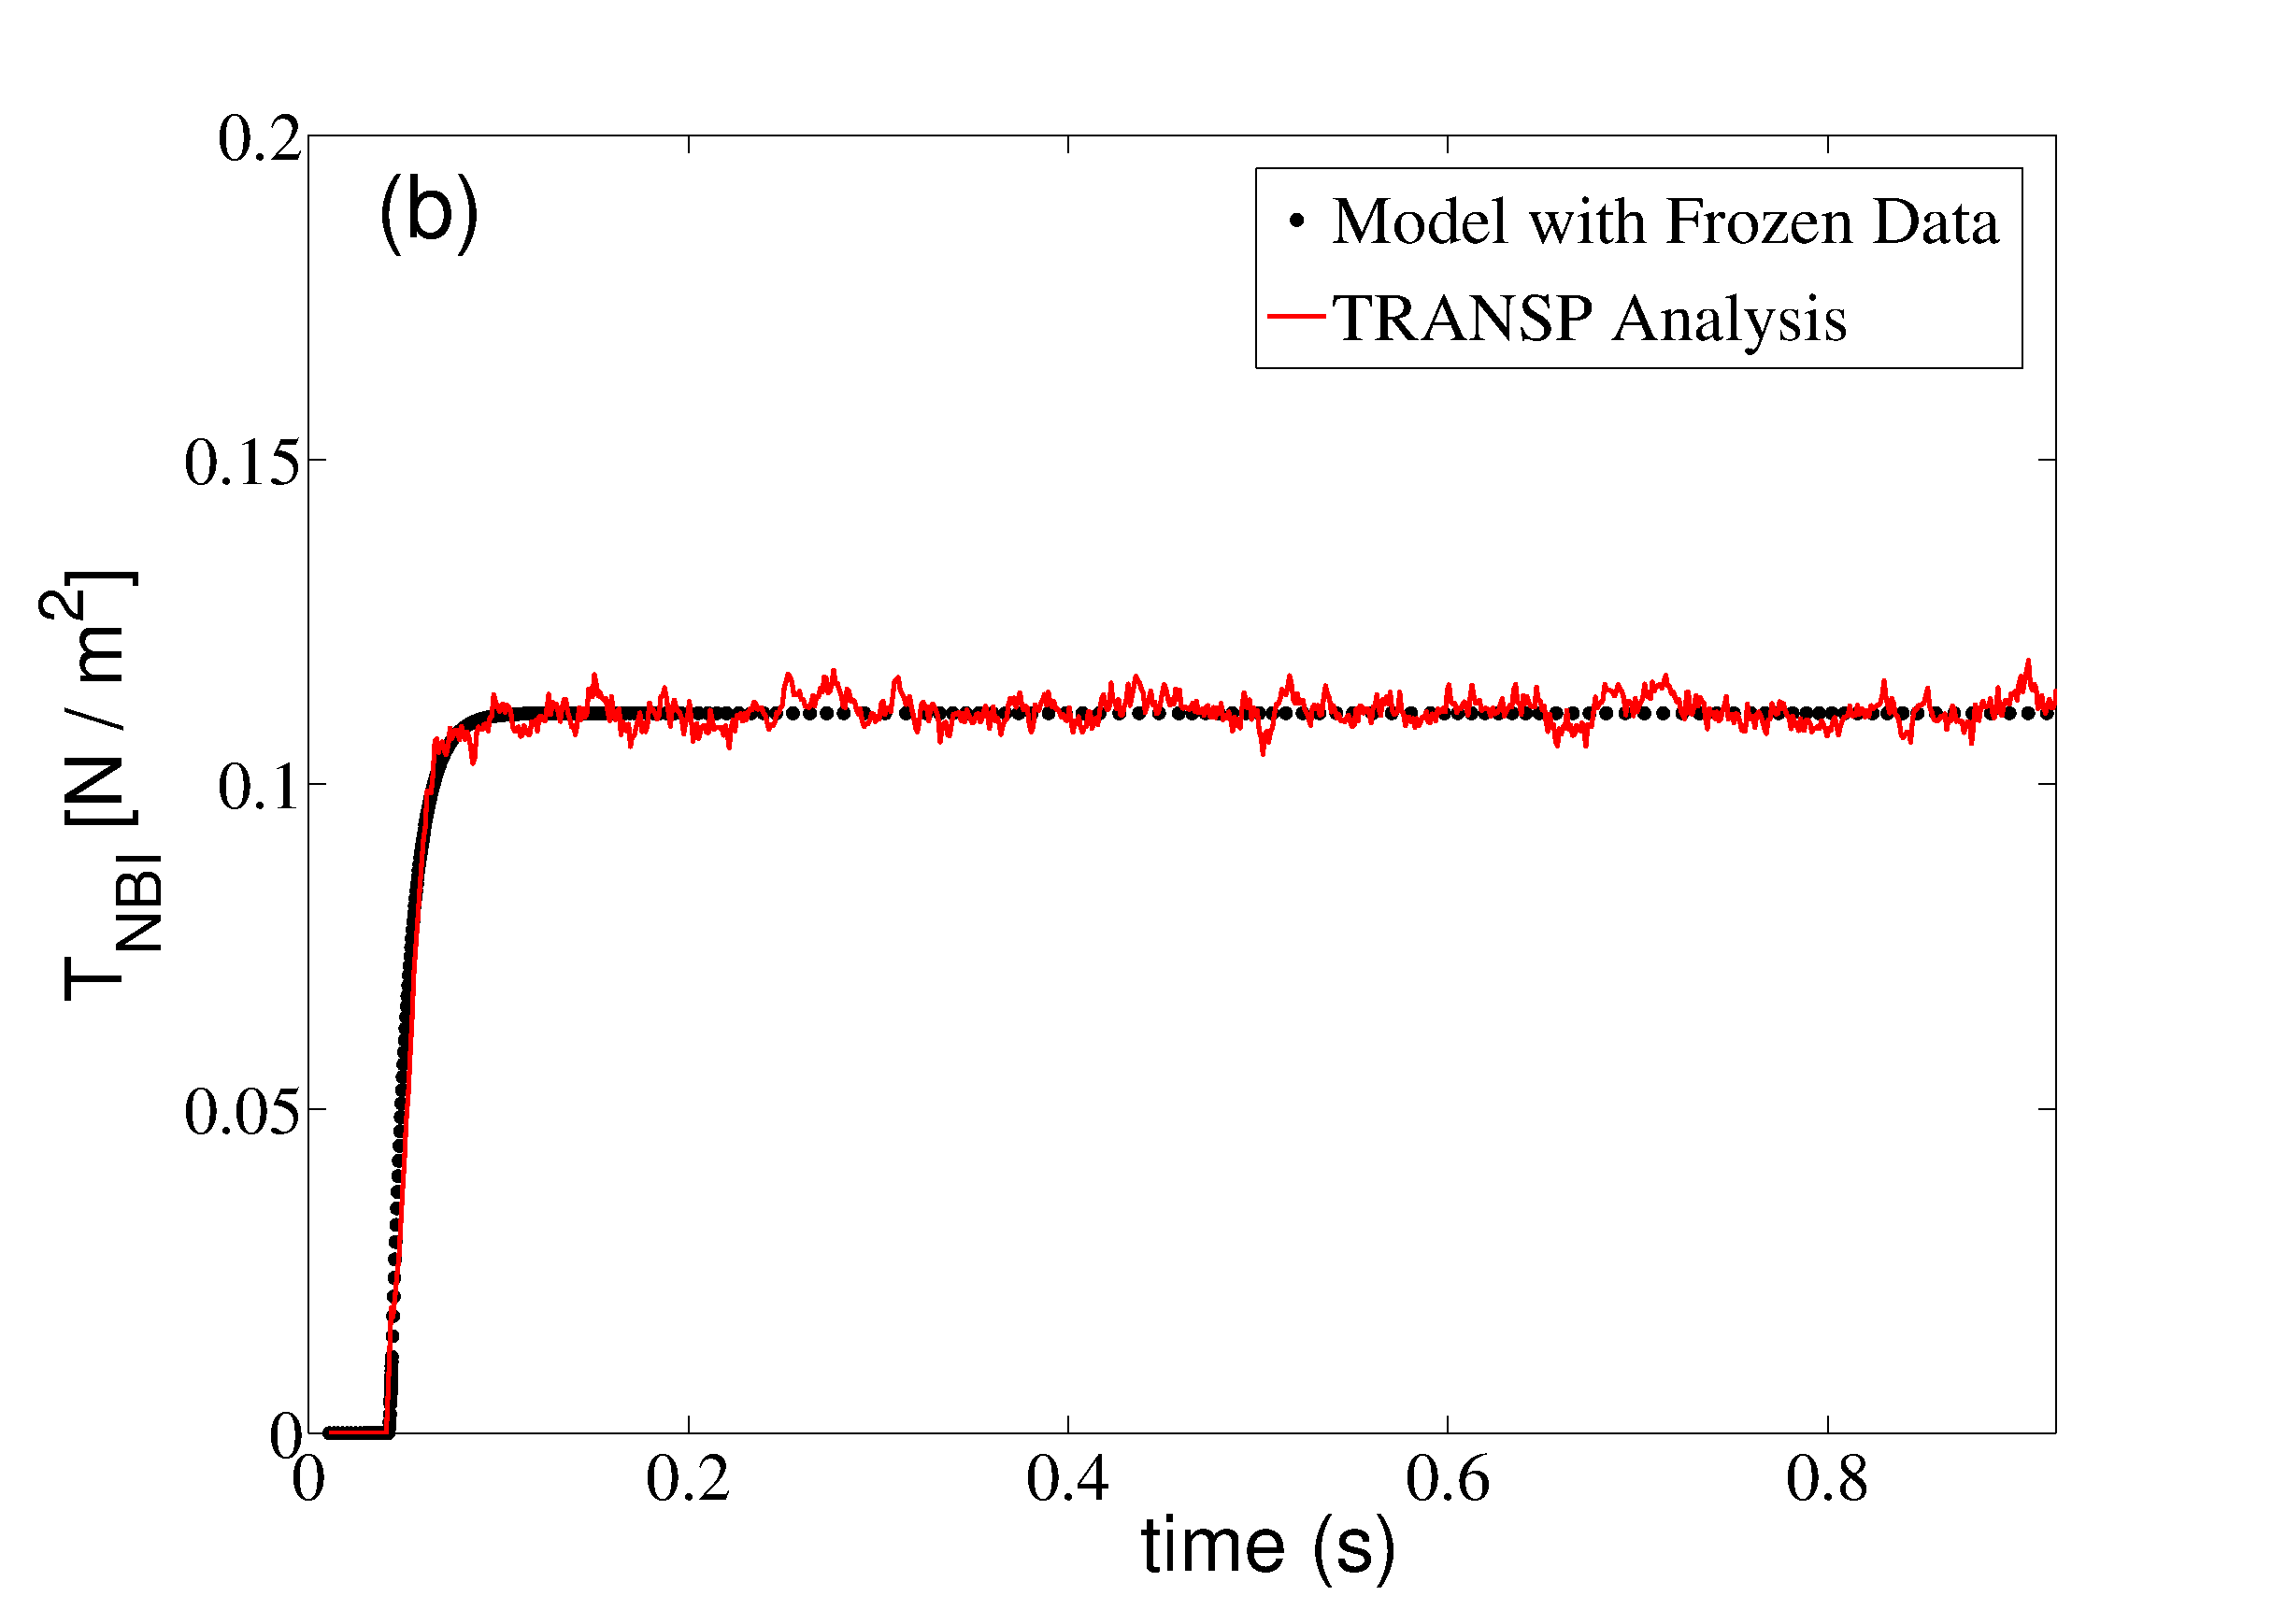
\includegraphics[width=0.5\linewidth]{imene_figs/Goum8}
\end{tabular}
\caption{(a) represents the spatial profile for the neutral beam torque ($F_\textrm{\tiny{NBI}} $) for plasma discharge 133367.  The shade represents the values of the function spanned over time interval $(0.45-0.92)$ seconds.  The time-average values are shown by the dashed black line (-~-) the frozen time values and its curve-fits are shown by the solid blue lines (-) and the red dots (o) respectively. (b) represents the corresponding spatial average of the torque generated for the same plasma discharge ($ \overline{T}_\textrm{\tiny{NBI}}$). The dotted (o) and  solid (-) lines represent the model simulated and TRANSP analysis reading, respectively.  Here ($\tau_\textrm{\tiny{NBI}} \approx 0.01 \textrm{s}$ and $\kappa_\textrm{\tiny{NBI}} \approx 2\times10^{-6} $)}
\label{fig:Fnbi}
\end{figure}
Figure~{\ref{fig:Fnbi}}(\emph{a}) shows the deduced profile $F_\textrm{\tiny{NBI}}$ of the torque generated by the neutral beams. The time-average data points have been curve fitted by a Gaussian to TRANSP analysis of this discharge using a least-squares method, showing good agreement.  Typical values for the curve-fit parameters are $a_\textrm{\tiny{NBI}} \approx 1$ and $\sigma_\textrm{\tiny{NBI}} \approx 0.25$.

The spatial average of the torque $\overline{T}_\textrm{\tiny{NBI}}(t)$ is related to the power input, $P_\textrm{\tiny{NBI}}(t)$, by a first order ordinary-differential equation, since the transmission of energy of the injected high-speed neutral atoms to torque is not instantaneous
\begin{equation}
   \frac{\partial \overline{T}_\textrm{\tiny{NBI}}}{\partial t}
   + \frac{\overline{T}_\textrm{\tiny{NBI}}}{\tau_\textrm{\tiny{NBI}}}  = \kappa_\textrm{\tiny{NBI}} P_\textrm{\tiny{NBI}}(t).
   \label{eq:nbi_time}
\end{equation}
Here $\tau_\textrm{\tiny{NBI}}$ is the exponential slowing down time of the fast neutral beam particles to impart energy to the bulk plasma and $\kappa_\textrm{\tiny{NBI}}$ is a scalar used to normalize the neutral beam power $P_{NBI}$.  
This  power allows variation of the toroidal momentum with certain  technical limitations such as its maximum value cannot go over 6\,MW.
Figure~\ref{fig:Fnbi}(\emph{b}) represents the solution of equation~(\ref{eq:nbi_time}) where the source ($P_\textrm{\tiny{NBI}}$) is fixed to 6\,MW or taken from TRANSP analysis, and compares it directly with the spacial averaging of the experimental NBI torque when the three NBI sources are on.

Although there is one neutral beam line, and three NBI sources, each with a slightly different aiming angle into the torus in the NSTX device, for simplicity these beams are considered as a single torque input.  When required, this assumption may be removed to generate three different torque inputs as functions of three power inputs.  For the current analysis, we only use one power input and one torque output to account for the neutral beam injection.

The performance of this neutral beam injection torque model is examined and compared with the more elaborate Monte Carlo modeling of the neutral beam torque in TRANSP analysis in Figure~\ref{fig:Fullnbi}. The simpler model described above for use in the controller agrees sufficiently well with the TRANSP simulation analysis.
\begin{figure}
\centering
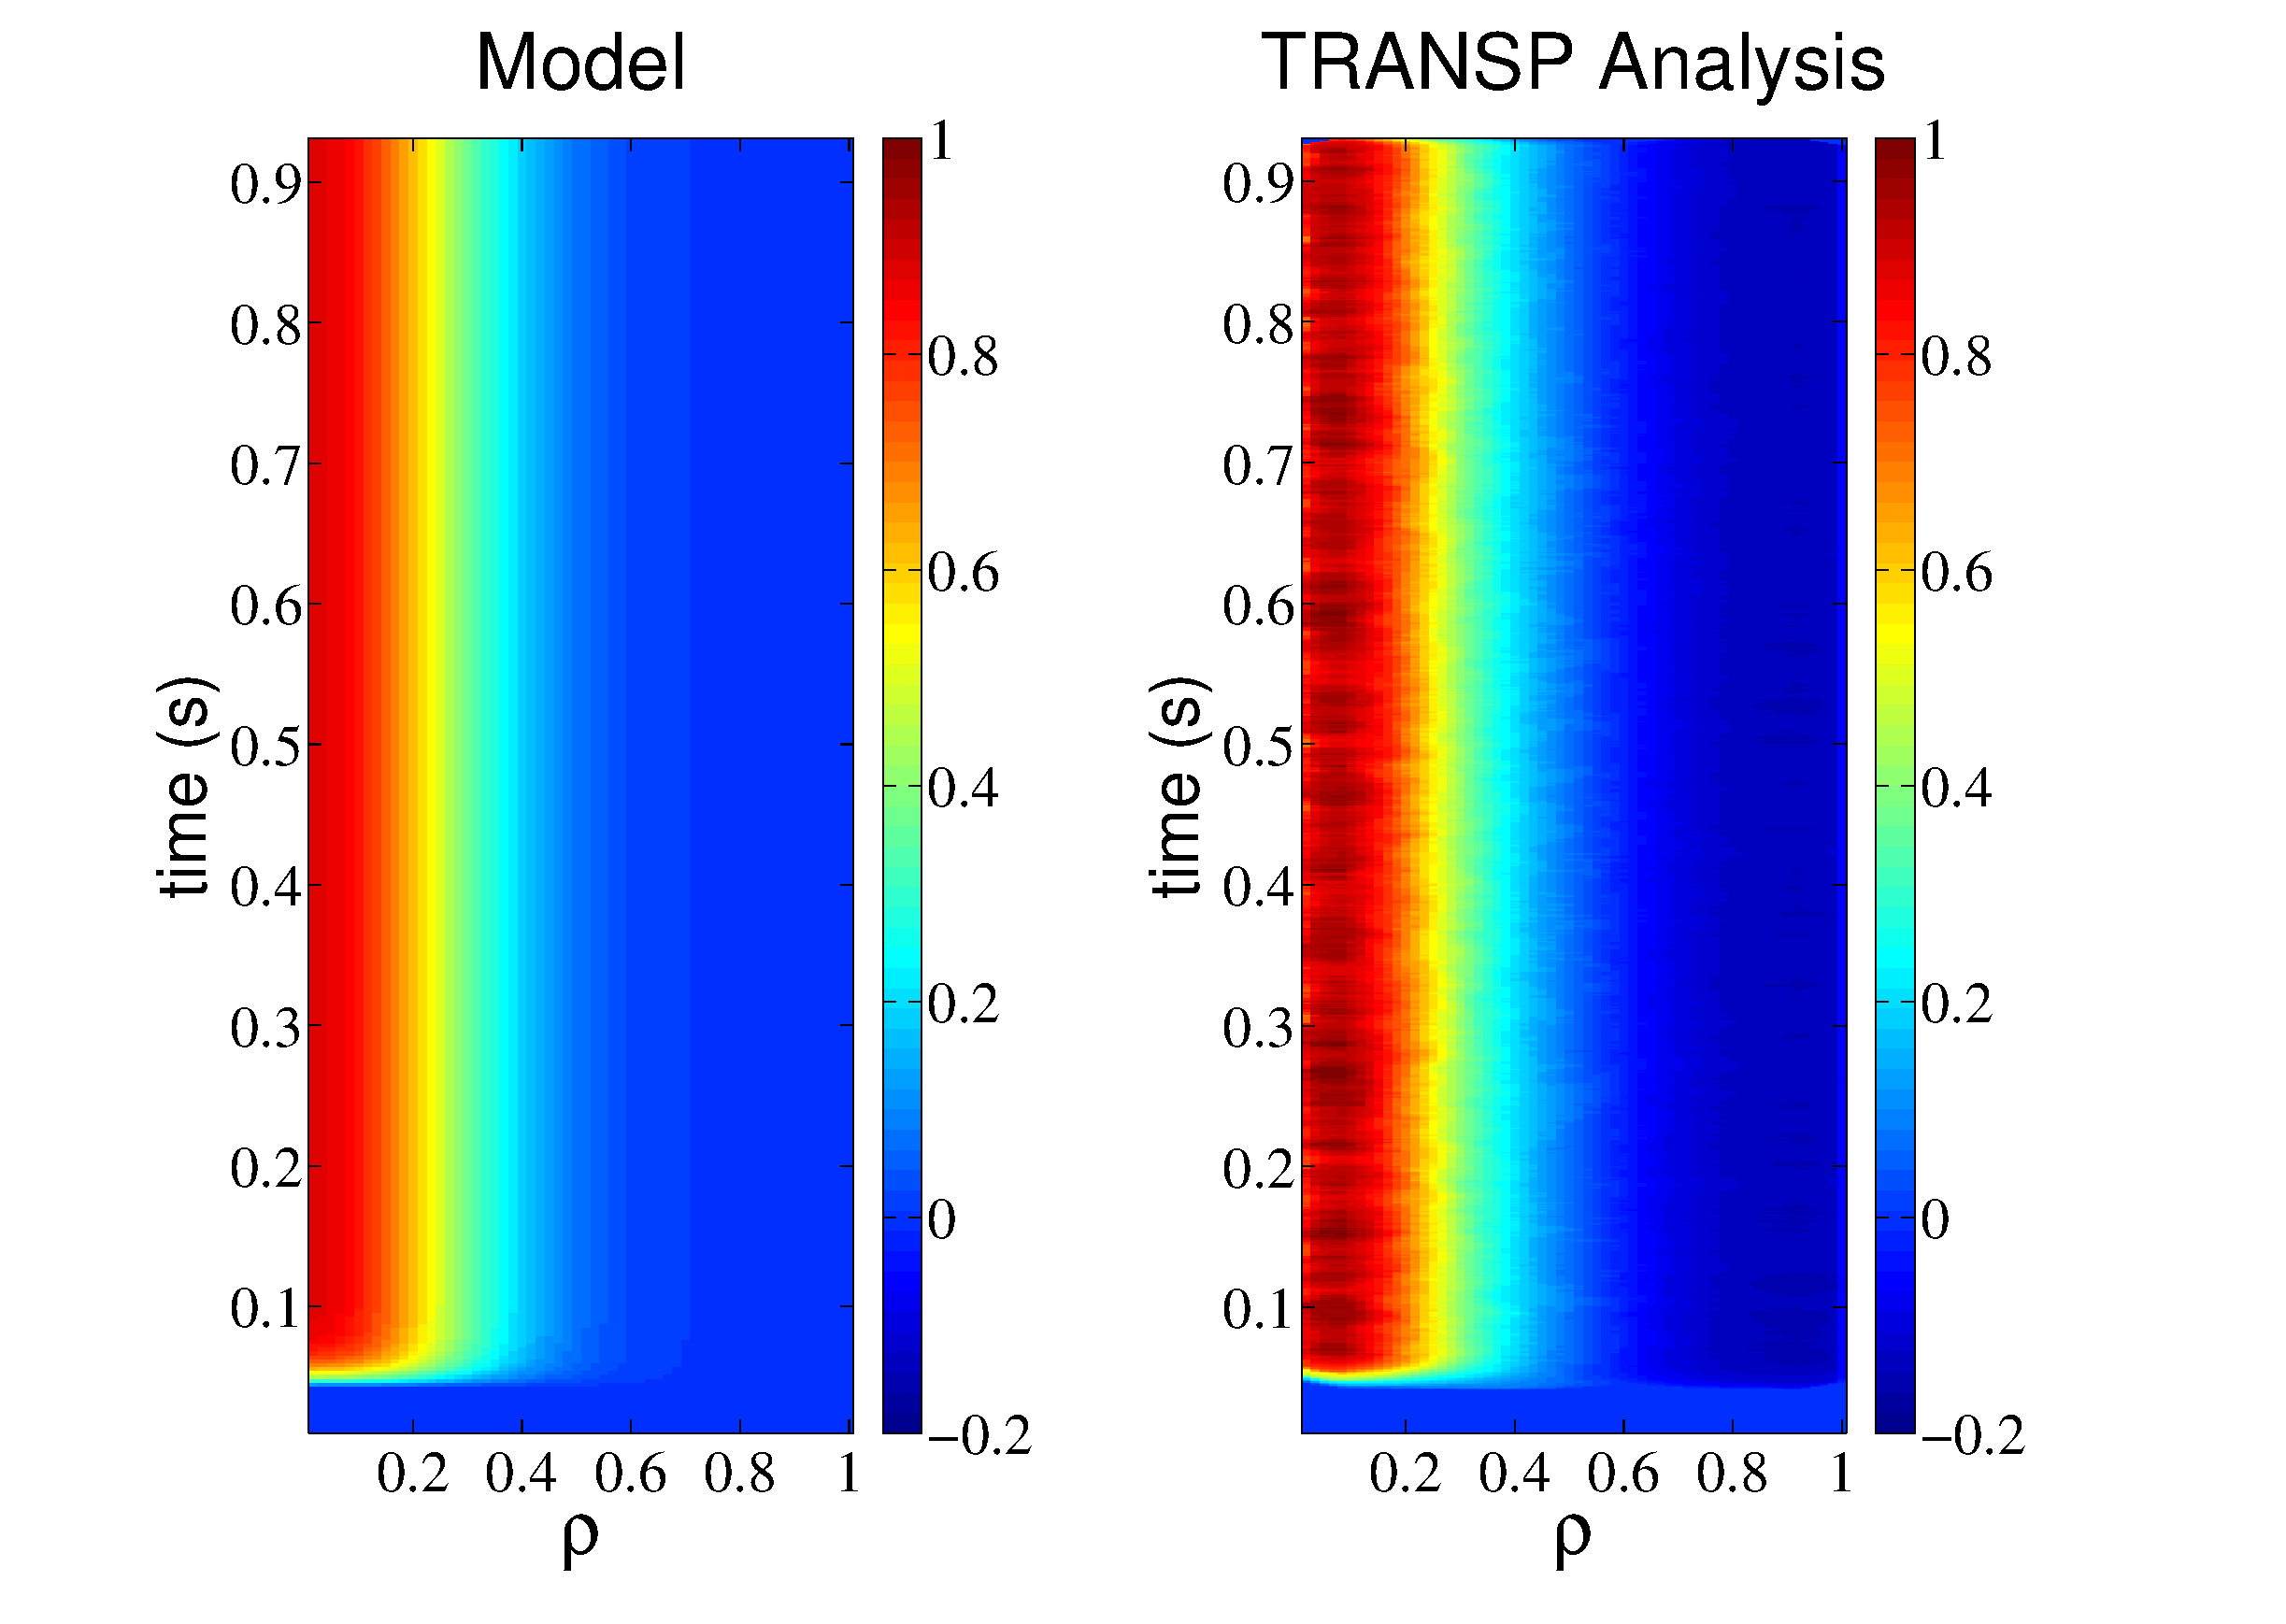
\includegraphics[width= \linewidth]{imene_figs/Goum9}
\caption{Comparison of the time evolution profile between the modeled NBI torque (from equations \ref{eq5}, \ref{eq6} and \ref{eq:nbi_time}) and the measured NBI torque from the TRANSP analysis.}
\label{fig:Fullnbi}
\end{figure}



\subsubsection{Neoclassical Toroidal Viscosity (NTV) actuator model}
 \label{TNTV}

Tokamaks usually have error fields or magnetohydrodynamic (MHD) activities present and these imperfections break the toroidal symmetry of the magnetic field and result in enhanced neoclassical toroidal plasma viscosity which then increases the rate of toroidal flow damping. The result will be a change of the edge rotation and shear. 

\begin{figure}
	\centering
   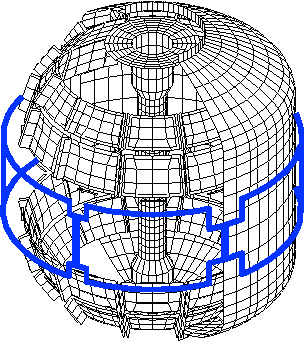
\includegraphics[width=0.6\linewidth]{imene_figs/pic_NTV}
\caption{Model representation of the three-dimensional coils (highlighted in blue) used to create the magnetic field that produces NTV in the NSTX device.}
  \label{pic_NTV}
\end{figure}
For the current one-dimensional toroidal momentum model, we aim to model the momentum loss due to the neoclassical toroidal viscosity in the toroidal average sense and base our model on the work done in \cite{Zhu06} from which we can design the NTV torque as the bilinear product of the coil (Figure~\ref{pic_NTV}) current squared ($ I^2$) with the toroidal momentum $\omega$ as follows
\begin{equation}
   T_\textrm{\tiny NTV}  (t, \rho) =  - K \, G(\rho) \,  \langle R^2 \rangle \:  I^2(t) \,\omega (t, \rho),
    \label{eqn:ntv}
\end{equation}
where $K$ is a constant and $G$ is a gaussian function.
\begin{figure}
  \begin{tabular}{cc}
     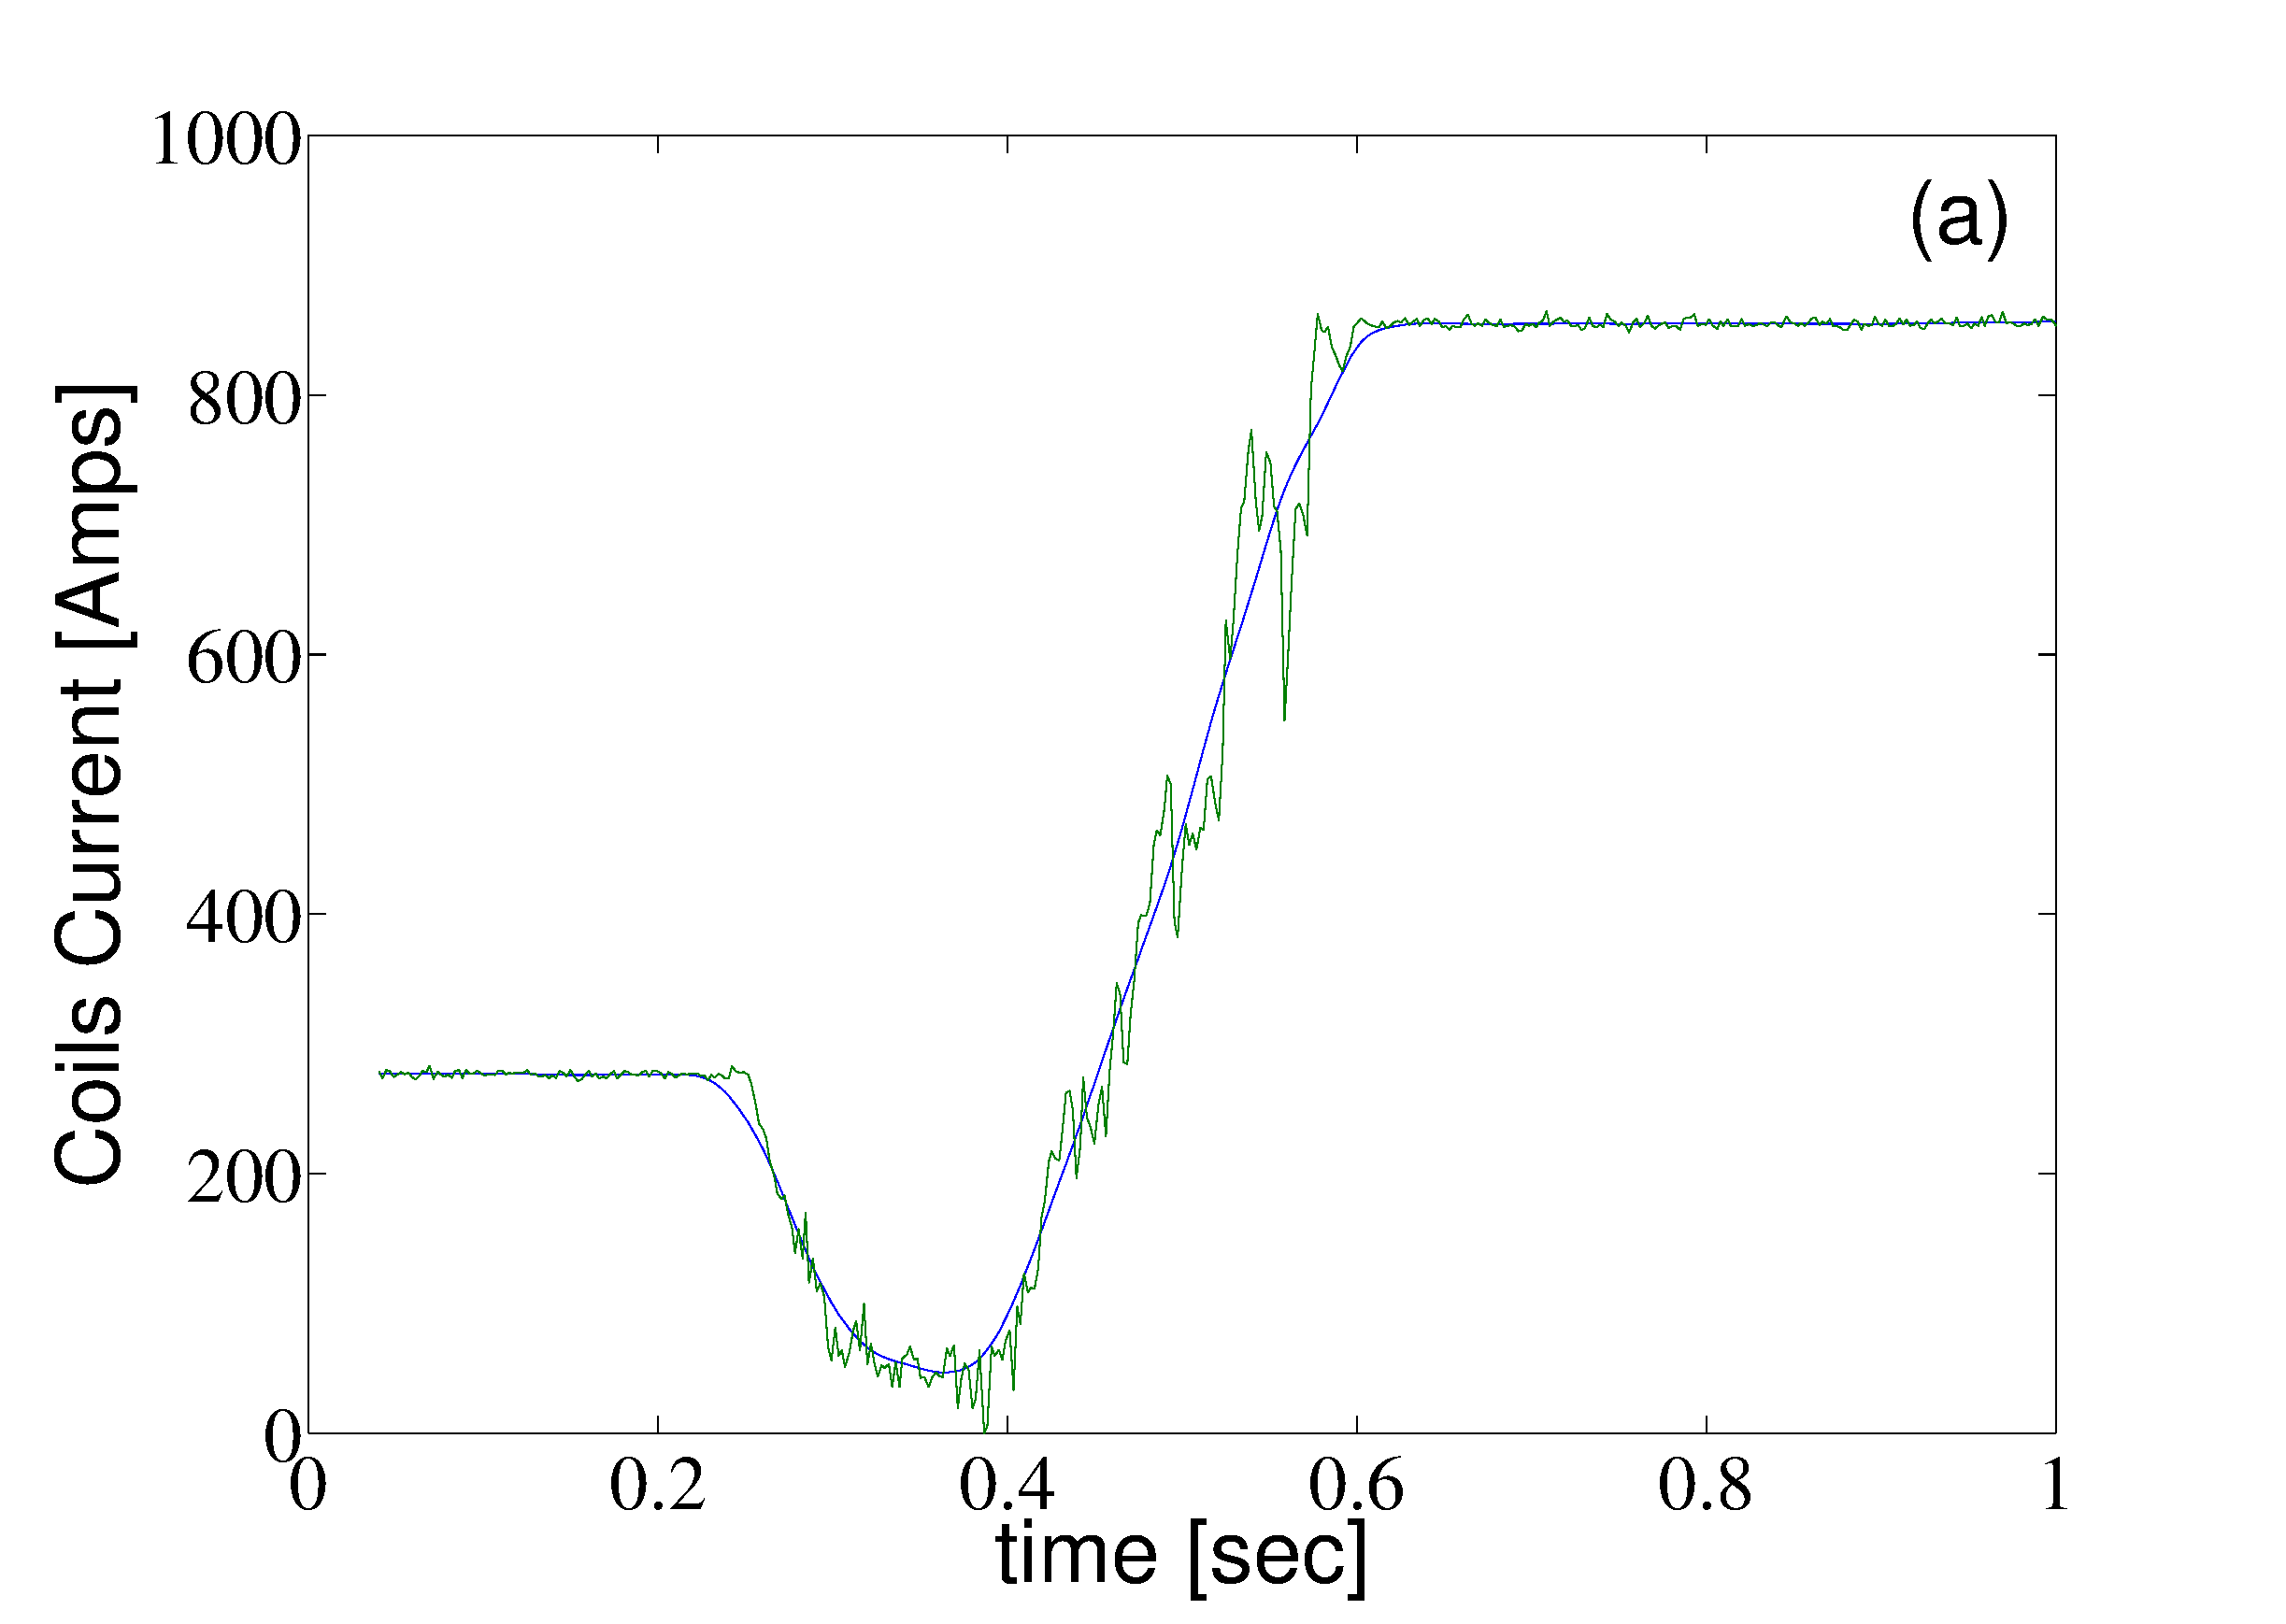
\includegraphics[width=0.5\linewidth]{imene_figs/current} &
   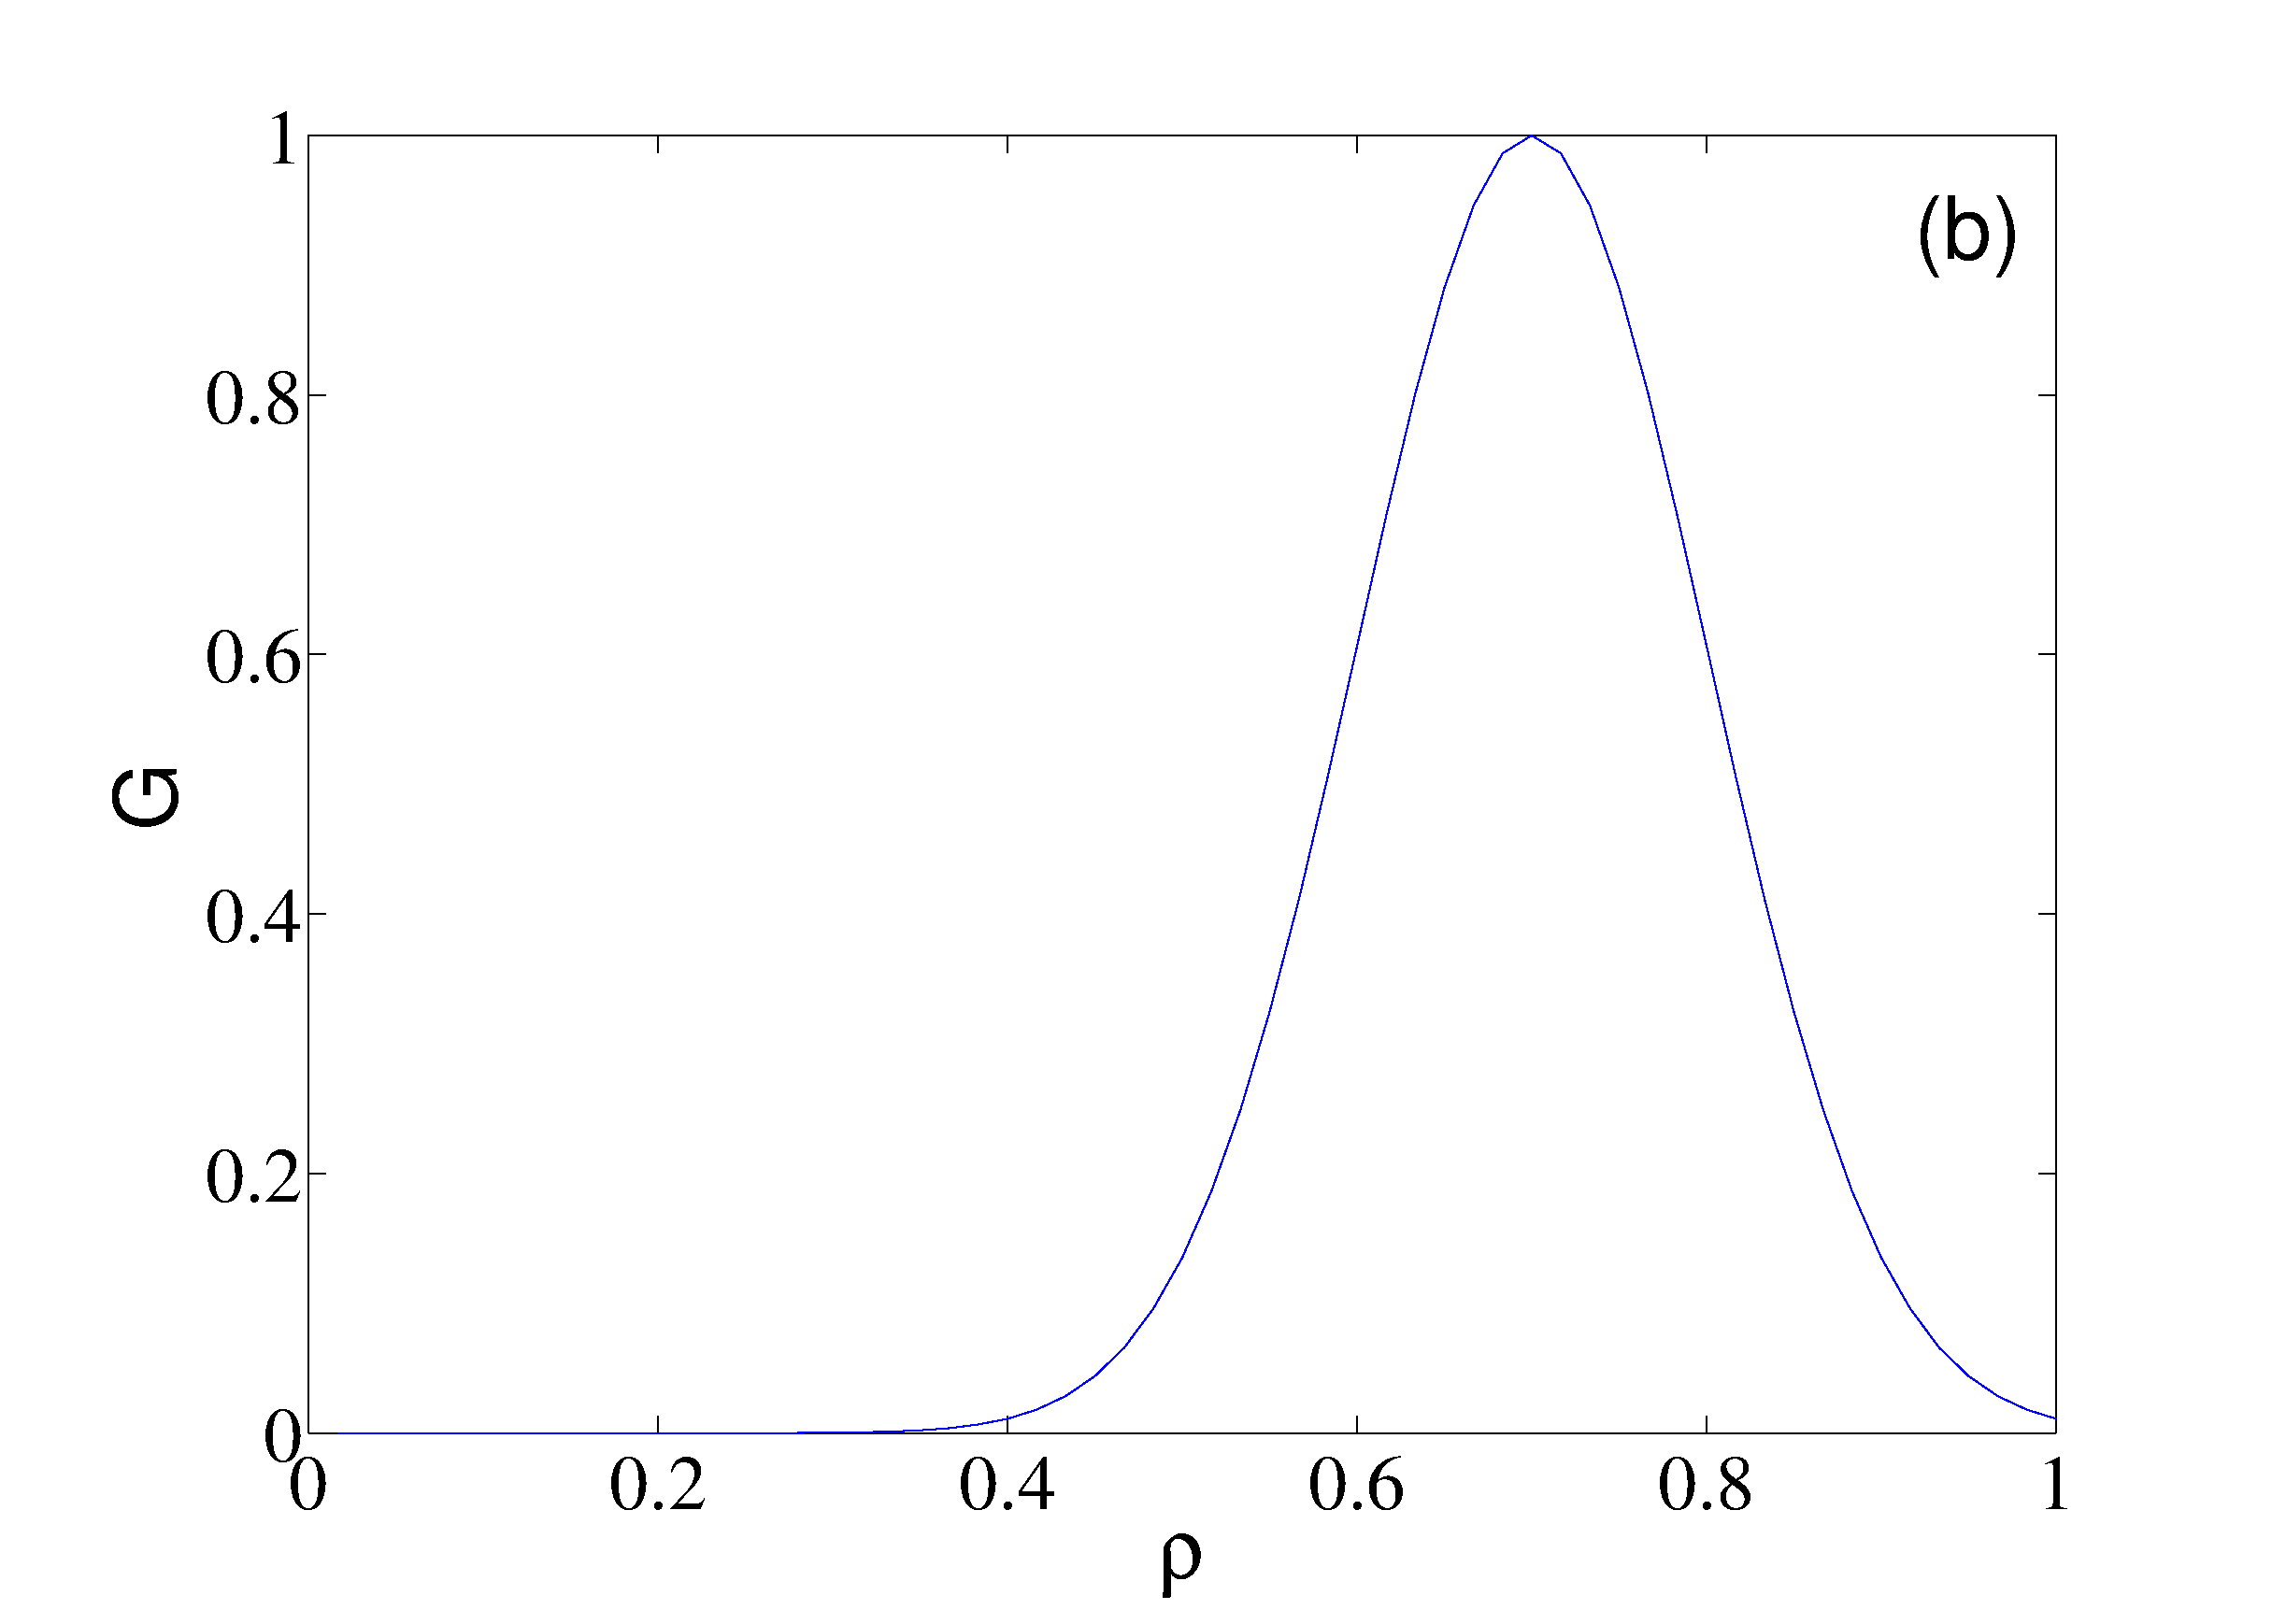
\includegraphics[width=0.5\linewidth]{imene_figs/gauss1}
  \end{tabular} 
\caption{ The temporal profile (current  in the coils) of torque $T_\textrm{\tiny{NTV}}$ for plasma discharges 133367 smoothed and unsmoothed (a), and the  spatial profile model $G$ of the neoclassical toroidal viscosity (b)  which is a Gaussian function. The green line represents the model from CHERS data and  blue lines represent the smoothed data.}
  \label{fig:current}
\end{figure}
The present model  will focus on the torque generated by the $n=3$ applied field "configuration", in which the current reverses direction in each of the six neighboring coils. Other applied field configurations are possible (e.g. configurations with dominant $n = 2$ component) and have experimentally produced effective NTV as well \cite{Sabbagh10}.
 
The approach in our model is to approximate the general shape of $T_\textrm{\tiny{NTV}}/\omega$ by a time-invariant spatial profile and a time-evolution of a scalar current, similar to the way $T_{NBI}$ was treated. The resulting model has the form  
\begin{equation}
   \frac{T_\textrm{\tiny{NTV}}(t,\rho)}{\omega(t,\rho)} = - G_\textrm{\tiny NTV}  (\rho) \, I^2(t),
\end{equation}
where
\begin{equation}
G_\textrm{\tiny NTV}  (\rho) = K \,  \langle R^2 \rangle \:G(\rho),
\end{equation}

\begin{figure}
\centering
\includegraphics[width=\linewidth]{imene_figs/Goum10} 
\caption{3D representation  of the NTV torque model where $\omega$ is taken from experimental measurements of ``frozen'' plasma discharge 133367}
\label{TNTV3D}
\end{figure}

and $G(\rho)$ is a gaussian function modeled in Figure~{\ref{fig:current}}(\emph{b}). Figure~{\ref{fig:current}}(\emph{a}) shows the current that flows into the coils for the plasma discharge  133367. We notice that the current is kept constant after $0.6$s. It should be noted that the actuator input here will be the current function (${I^2}\textrm(t)$). 
Using the experimental rotation profile, the modeled NTV torque is shown in Figure~\ref{TNTV3D}.

\subsection{Testing and comparing the model}

In this subsection, the rotation evolution generated by the data-driven model using a specific discharge is compared first to TRANSP analysis of the same discharge. Second, the same data-driven model is compared to TRANSP analysis of a different discharge using analogous inputs of the new discharge in the model to demonstrate that the qualitative and quantitative behavior of the rotational plasma momentum can be captured.  The models are integrated in time based on the method of \cite{Skeel90} for  the spatial discretization of parabolic equations in one space variable and are computationally inexpensive due to the one-dimensional nature of the model.  This is an important point for control in general and real-time feedback control in particular. 
\subsubsection{Model vs TRANSP for the same plasma discharge}
Given two points of measurements of rotation (outputs), one near the core, the other one towards the edge of the tokamak (more details in the next section); the model is first run with only the NBI actuator on ($6$\,MW), then at $t=0.5$\,s, the NTV actuator is turned on. 

\begin{figure}
\centering
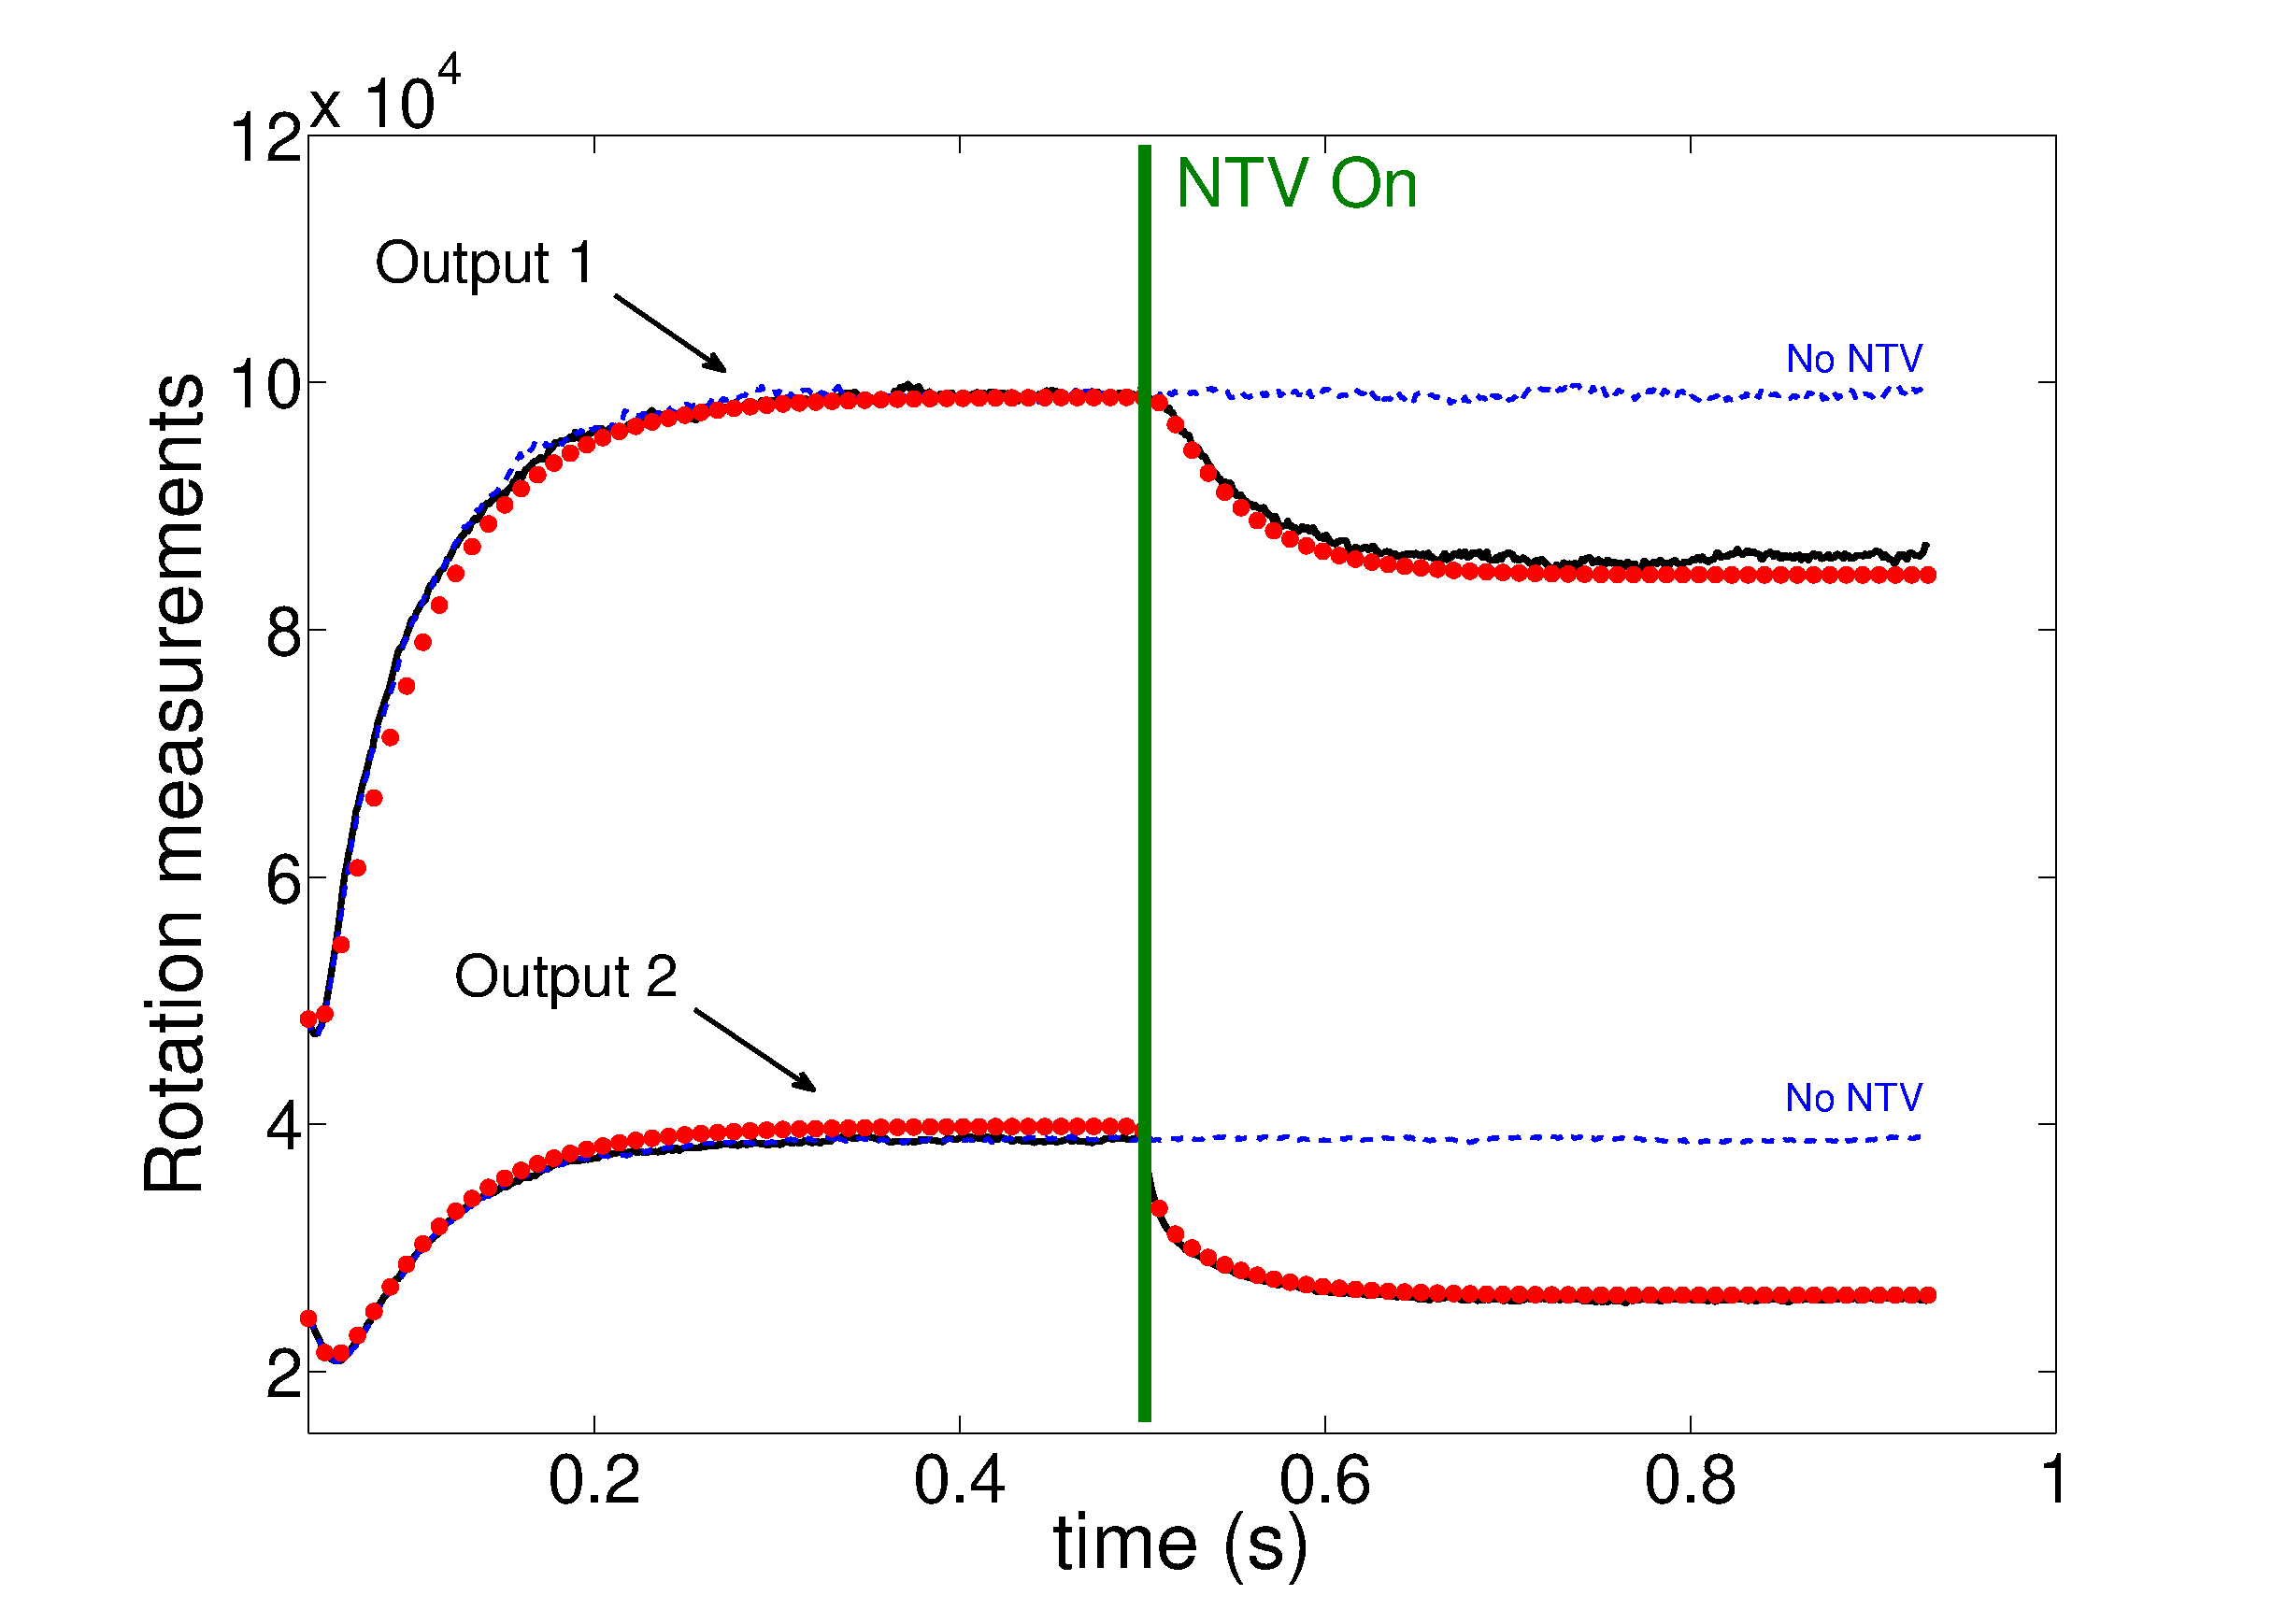
\includegraphics[width=\linewidth]{imene_figs/Goum12} 
\caption{Two rotation measurements with NBI and NTV actuators activated at $t=0$\,s and $t=0.5$\,s respectively, which are represented by the solid black line (-) (TRANSP analysis) and red dots (o) (simplified model) respectively. The blue dashed line (-~-) represents the steady values of these outputs reached if only NBI is ON.}
\label{Goum12}
\end{figure}

Figure~\ref{Goum12} shows these rotation measurements for the simplified model (red dots) compared against TRANSP analysis (solid black line) when the NBI and NTV actuators are activated at $t=0$\,s and $t=0.5$\,s respectively. The blue dashed line shows the steady values reached when only NBI is activated. It shows that the model is a good approximation of the TRANSP analysis model.



\subsubsection{Model vs TRANSP for a different plasma discharge}

The simplified model is now compared to the TRANSP analysis of a different plasma discharge ($133743$) as shown in Figure \ref{fig10}. the relative error between the model and experimental data (which is the difference between the experimental and the model rotation divided by the mean of the spatial average of the experimental rotation data) is also shown in  the same figure.

For all the models, the initial condition is set to be the experimental rotational frequency at  time $t=0.4$\,s after the start up ($t=0$) and when the plasma reaches the H-mode.

An exact plasma model is not a major concern as feedback control can be performed to tolerate errors in the model. The key is to ensure the model does not deviate drastically from the actual profile in order to prevent control system instabilities from dominating plasma physics dynamics.

This simplified model (derived plasma discharge 133367) has been extensively validated against other plasma discharges in NSTX analysis (here showing 133743). The error remains acceptable starting with less than 20\% for the  experimental data 133743 where the original model was maintained the same, only the density and the input torques were updated. The error does not exceed 30\% for other experimental comparisons which is tolerable for plasma rotation control.

The overall behavior of the plasma is captured qualitatively very well using the simplified model of equation~\ref{model0}. 

\begin{figure}
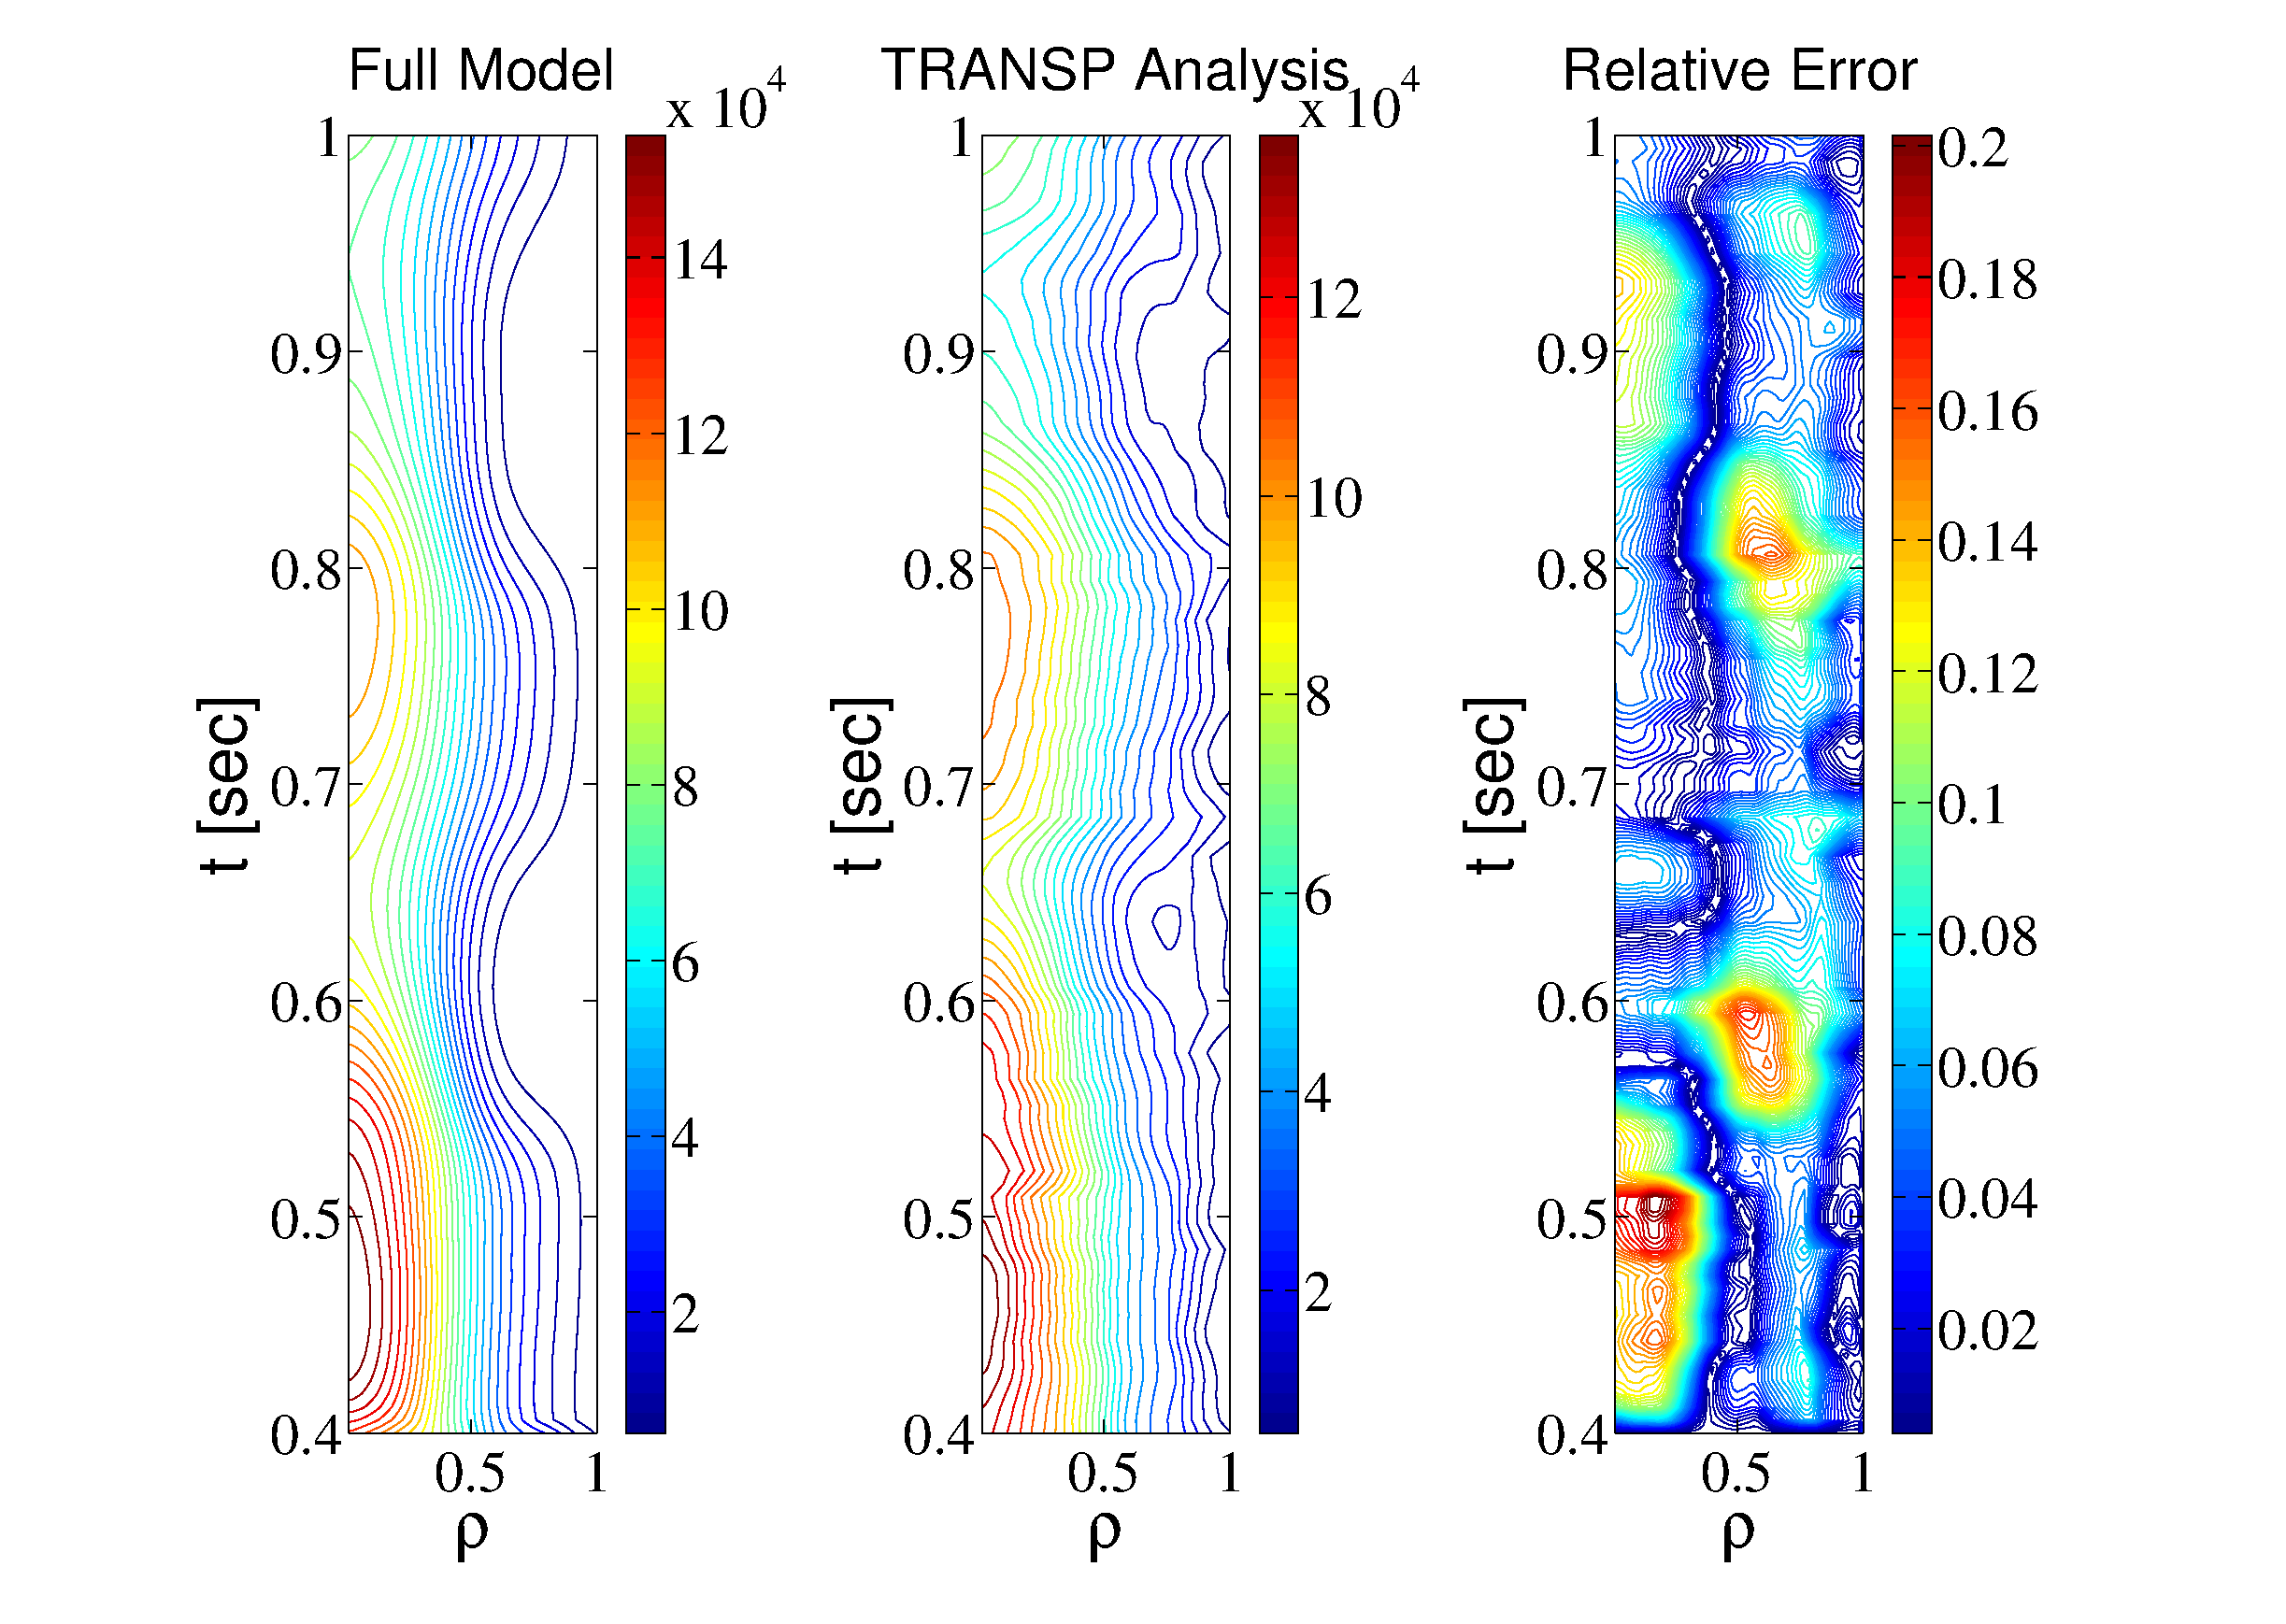
\includegraphics[width=\linewidth]{imene_figs/bessel_comp} 
\caption{Comparison of the rotational frequency $\omega$ from the simplified model vs experiments for plasma discharges 133743  and the representation of its respective relative errors.}
\label{fig10}
\end{figure}

\subsection{Reduced order model using Bessel functions}

Among many model reduction techniques, such as singular perturbation or Hankel norm reduction methods, the projection-based method, which involves projection of a model onto a set of modes, is a widely used approach. These may be global eigenmodes of a linearized operator \cite{Akervik07}, modes determined by proper orthogonal decomposition (POD) of a set of data, or variants of POD modes \cite{Holmes97}. 

It can be noticed from the mathematical structure of the momentum diffusion equation~(\ref{model0}), that the diffusion part looks like a Laplacian operator in cylindrical coordinates, thus the Bessel functions will be the natural choice for the basis. 

Recall that the Bessel modes are constructed as different versions of the same Fourier-Bessel function of the first kind $J_{\alpha}$, where the argument to each version $n$ is differently scaled, according to
\begin{equation}
(J_{\alpha})_n (x) = J_{\alpha} \left(  \frac{ k_{\alpha,n}}{L} x \right),
\label{defmod}
\end{equation}
where $ k_{\alpha,n}$ is a root, numbered $n$ associated with the Bessel Function $J_{\alpha}$. $L$ is a length constant assumed to equal unity as the spatial variable varies between 0 (at the core) and 1 (at the edge of the plasma). The variables $a_n$ are the assigned coefficients. The toroidal rotation $\omega$ can thus be written as 
\begin{equation}
\omega(\rho,t)  = \sum_{n=0}^{\infty} a_n(t) \, J_{\alpha} \left( { k_{\alpha,n}} \rho \right),
\label{decomp}
\end{equation}
 with
 \begin{equation}
a_n(t) = \frac{\langle \omega(\rho,t), \left(J_{\alpha} \right)_n \rangle }{\langle  \left(J_{\alpha} \right)_n ,  \left(J_{\alpha} \right)_n   \rangle},
\end{equation}
and where the scalar product is defined as 
\begin{equation}
\langle f,g \rangle =   \int^1 _0 \rho \, f(\rho) \, g(\rho) \, d\rho.
\end{equation}
By matter of respecting the boundary conditions given in equation~(\ref{bc0}), we consider the particular case of $\alpha = 0$, this reduces equation~(\ref{decomp}) to
\begin{equation}
\omega(\rho,t)  = a_0(t) + \sum_{n=1}^{r} a_n(t) \, J_{0} \left(  k_{0,n} \rho \right),
\end{equation}
with
\begin{equation}
a_0 (t) = {2} \int^1 _0 \rho \, \omega(\rho,t) \, d\rho.
\end{equation}
and $r$ being the number of Bessel modes chosen to represent $\omega$.

This Bessel decomposition is now applied on the simplified model defined by equation~(\ref{model0}). Figure~\ref{bessel1} compares the three model simulations, one is taken from TRANSP analysis of the experimental measurement of the toroidal rotation, the other model is simulated in real space dimension and the third one solved spectrally by projecting the original model on only 4 Bessel modes. It can be noticed that only 4 Bessel modes are sufficient for capturing most features of the dynamics.
\begin{figure}
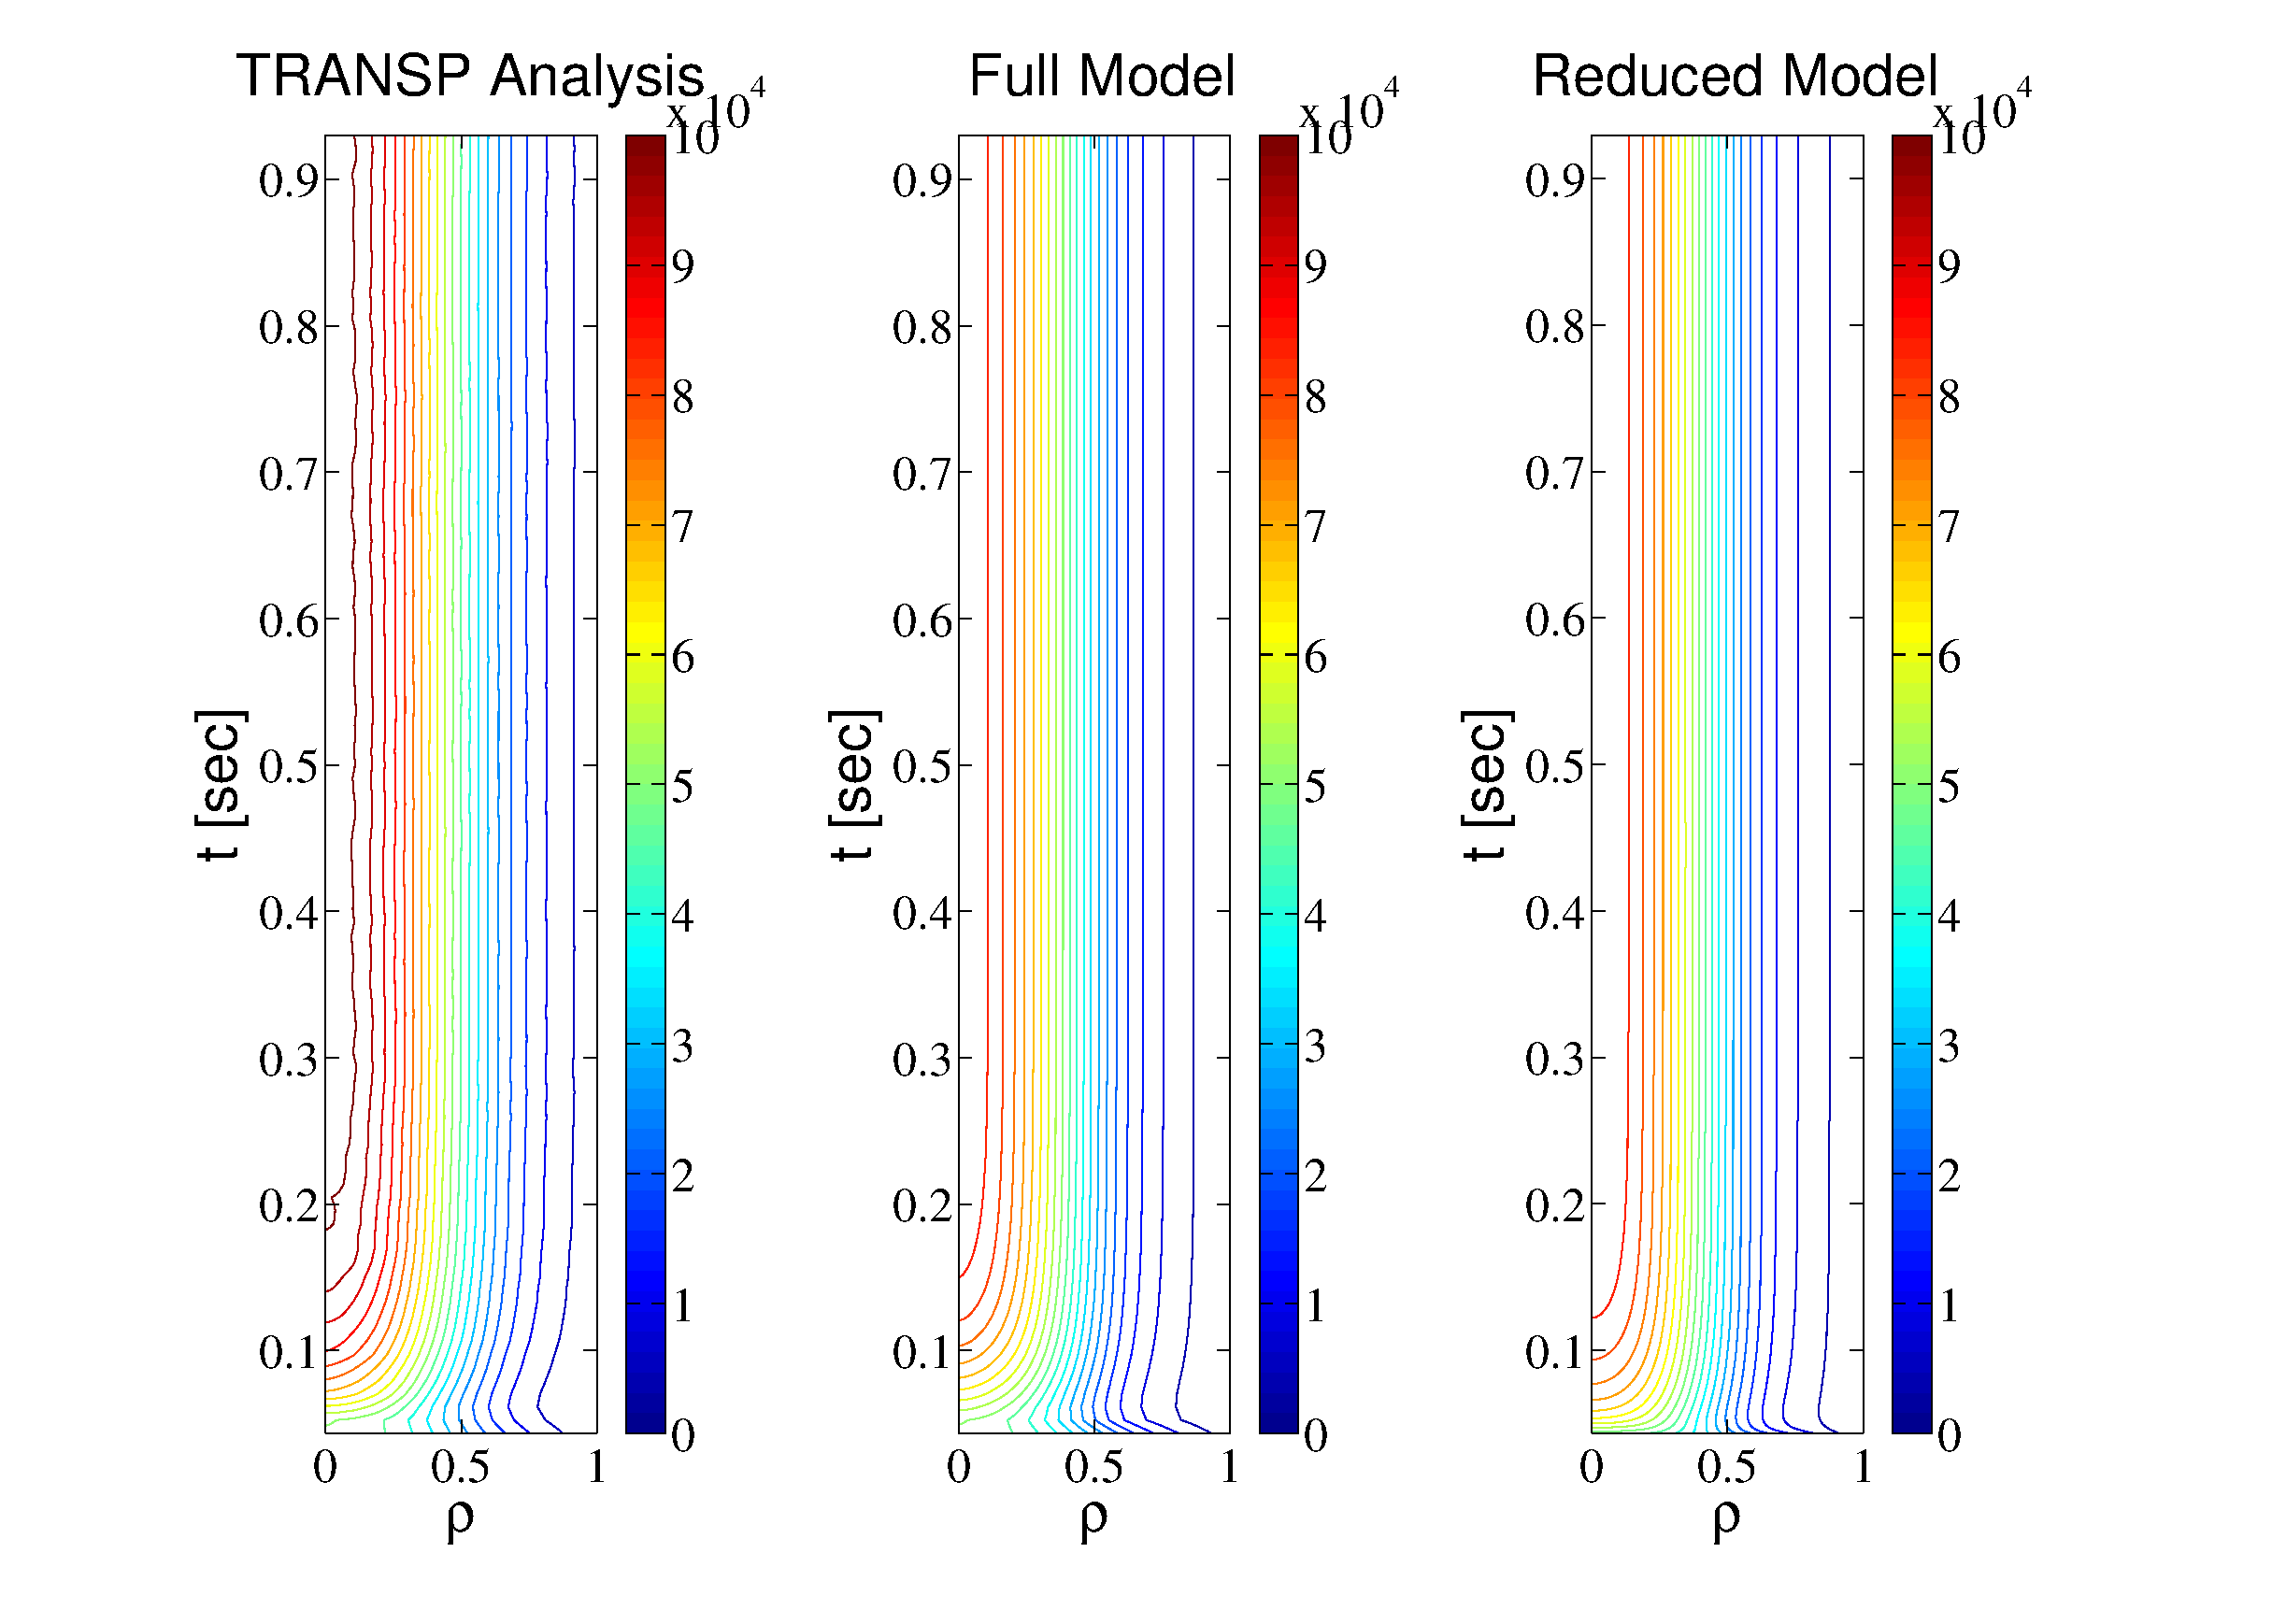
\includegraphics[width=\linewidth]{imene_figs/bessel11n} 
\caption{comparison of spectral simulation of the toroidal rotation using 4 Bessel modes (right) with the full nonlinear simplified model using 60 points of discretization for plasma discharge 133367 (middle) and the rotation from TRANSP analysis (left). }
\label{bessel1}
\end{figure}

\section{Linear rotation plasma control}
 \label{LRPC}
 
 The purpose of this section is to demonstrate that standard model-based control techniques may be used to guide an experimental plasma rotation profile to track a desired reference. Some approaches on how controllers can be designed to achieve a desired shape with a reasonable response time are presented in the following sections.
 
 Recall that the two actuators available to the controller are the (NBI) beams power and the coil current producing NTV.
In this case, a state-space realization is derived and linear quadratic regulators are used to design a feedback controller that is optimal in minimizing a prescribed quadratic cost function (details are explained below).

\subsection{State space realization}
In order to be able to use linear control tools, a linearized state-space realization of the original simplified nonlinear system has to be built.
Recall that the original simplified system is given by equation~(\ref{model0}).
Let $\omega_0$ be the steady state reached for the given beam power $ P_0$ and coil current $I_0$. The linearization around this steady state profile can be written as
\begin{eqnarray}
\omega (t, \rho) &= \omega_0 (\rho) + \omega_1(t, \rho), \\
I (t) &= I_0 + I_1(t),\\
P_\textrm{\tiny NBI} (t) &= P_0 + P_1(t),
\end{eqnarray}
where $ \omega_1$ , $ I_1$ and $P_1$ are the respective perturbations to the equilibria $\omega_0$, $I_0$ and $P_0$.
By plugging in these equations into equations~(\ref{eqn:model_nbi_fix}) through (\ref{eqn20}) and simplifying, we obtain
\begin{equation}
\frac{\partial}{\partial t}   \left[\! \begin{array}{c}  \omega_1 \\ \overline{T}_\textrm{\tiny{NBI}} \end{array}\!\right]
  ={ \left(\! \begin{array}{cc} a_{11}  & a_{12} \\ 0 & a_{22} \end{array} \! \right)} \left[\! \begin{array}{c} \omega_1 \\ \overline{T}_\textrm{\tiny{NBI}}    \end{array}  \!\right] + \left(\! \begin{array}{cc} b_{11}  & 0 \\ 0 & b_{22}    \end{array}  \!\right) \left[\! \begin{array}{c}  I^2_1 \\ P_1\end{array}\!\right]
\label{SSR}
\end{equation}
 where
 \begin{eqnarray}
 a_{11} =  \frac{1}{n m \left<R^2\right>} \left[ \left( \frac{\partial V}{\partial\rho}\right)^{-1}
   \frac{\partial}{\partial \rho} 
   \left[\frac{\partial V}{\partial \rho}(n m)\chi_\phi 
   \left< R^2 (\nabla \rho)^2\right> 
   \frac{\partial}{\partial\rho}\right]-K G(\rho) \langle R^2 \rangle  I^2_0 \right]  \nonumber \\
 a_{12} =  \frac{ F_\textrm{\tiny{NBI}}(\rho) }{n m \left<R^2\right>}\nonumber \\
 a_{22} = - \frac{1}{\tau_\textrm{\tiny{NBI}}}  \nonumber \\  
 b_{11} = - \frac{1}{n m \left<R^2\right>} K G(\rho) \langle R^2 \rangle  \omega_0 \nonumber \\
 b_{22} = \kappa_\textrm{\tiny{NBI}} \nonumber
 \end{eqnarray}
 The above system of equations are spatially discretized at a set of $n-2$ discrete points between $\rho \in (0,1)$ to generate a state-space realization. The boundary points $\rho_1 = 0$ and $\rho_n =1$ are excluded since the boundary conditions are prescribed. With this spatial discretization, the system can be represented in the standard state-space form:
\begin{eqnarray}
 \dot{x}_1 &= A x_1 + B u_{1} ,\label{eqn:state-space1} \\
 y_1 &= C x_1, \label{eqn:state-space2} 
\end{eqnarray}
where $x_1 = [  \omega_1(\rho_2),  \omega_1(\rho_3), ...,   \omega_1(\rho_{n-1}), \overline{T}_\textrm{\tiny{NBI}}(t)     ] \in \mathbb{R}^{n-1}$ is the perturbed state $  \left[ \omega_1 , \ \ \overline{T}_\textrm{\tiny{NBI}}(t)  \right]$, $u_1 \in \mathbb{R}^p$ is the perturbed input $\left( I^2_1, \ \  P_1 \right)$ and $y_1 \in \mathbb{R}^q$ is the perturbed output (sensor measurements from their equilibrium values).
Here, there are two actuators ($p=2$), one power input for the neutral beams and another one for the coil current producing the NTV.
The outputs $y_1$ correspond to the sensor measurements of the plasma toroidal rotation. Here, two measurements are taken, one near the core and one towards the edge of the plasma ($q=2$).

The matrices $A \in \mathbb{R}^{\, (n-1) \times (n-1)}$, $B \in \mathbb{R}^{\,(n-1) \times p}$, and $C \in \mathbb{R}^{\, q \times (n-1)}$ are respectively called the dynamics, control and sensor matrices.
Because the two measurements are pointwise, the matrix $C$ is composed of zeros with a single one on each line.

The state space realization can go one step further by using the spectral decomposition described above (Bessel functions) and projecting the partial state $ \omega_1$ on the $r$ chosen Bessel functions, the state $ \omega_1$ will then reduce to the $(r+1)$ Bessel coefficients of the projection $(a_{1_0}, a_{1_1}, ..., a_{1_r})$, the state-space realization will have the reduced dimensions of $A \in \mathbb{R}^{\, (r+2) \times (r+2)}$, $B \in \mathbb{R}^{\,(r+2) \times p}$, and $C \in \mathbb{R}^{\, q \times (r+2)}$.

\subsection{Non-zero target state}
Once the state-space realization is obtained, the goal is to force the shape of the plasma rotation profile to reach a target state $x_d$ such that the sensor output $y_d$ matches a reference signal $r_d$. In the final implementation, all one should have to prescribe is $r_d$ (e.g., plasma rotational frequency values at certain locations). The target state $x_d$ and the corresponding input $u_d$ are found by solving equations~(\ref{eqn:state-space1}) and (\ref{eqn:state-space2}) at steady state
\begin{equation}
\left[\! \begin{array}{c}  x_{1d} \\ u_{1d}\end{array}\!\right]
  ={ \left(\! \begin{array}{cc} A  & B \\ C & 0 \end{array} \! \right)}^{-1} \left[\! \begin{array}{c} 0 \\ I    \end{array}  \!\right] r_{1d} = \left[\! \begin{array}{c} N_x \\ N_u    \end{array}  \!\right] r_{1d},
\label{steadystate}
\end{equation}
where 
\begin{eqnarray}
 x_{1d}  &= x_d - x_0, \\
 u_{1d}  &= u_d - u_0, \\
 r_{1d}  &= r_d - r_0 ,
\end{eqnarray}
and $\left( x_0, u_0  \right)$ is the equilibrium point around which the system is linearized, and $r_0$ the corresponding measurement values of $x_0 = \left( a_{0_0},a_{0_1}, ... , a_{0_r} ,  T_0 \right)$. 
 
\subsection{Rotational control design} 
Once the target states $\left( x_{1d} , u_{1d} \right)$ are established, the controllers are designed based on the reduced model dynamics, then applied to the full-dimensional linearized model, and finally tested on the original nonlinear model to determine if the controller can suppress disturbances and reach the desired profile in the vicinity of the equilibrium.


\subsubsection{Full-state feedback control design} 

When the reduced-order model (in Bessel basis) is obtained, a feedback control law can be constructed as
\begin{equation}
   u_1 = u_{1d} - K(x_1 - x_{1d}) = - Kx_1 + Fr_{1d},
   \label{eqn:ctrllaw_ff}
\end{equation}
where $K$ is the feedback control gain to be determined from control design and $F = N_u + K N_x$ is the feedforward gain.  Therefore, the resulting closed-loop system can be written as
\begin{eqnarray}
      \dot{x}_1 &= (A-BK) x_1 + BF r_{1d}, \\
      y_1 &= C x_1.
\end{eqnarray}
In order to design the controller from equation~(\ref{eqn:ctrllaw_ff}), we have to choose the gains $K$.
A  standard linear control technique (linear-quadratic regulators) is used in order to determine those gains while minimizing a quadratic cost function of the form:
\begin{equation}
 \mathcal{J} = \int_{t_0}^\infty \left( x^T Q x + u^T R u \right) dt,
 \label{bel}
\end{equation}
where $Q\ge 0$ and $R>0$ are symmetric, positive (semi-)definite weight matrices. $Q$ will be chosen to be equal to $a \, C^{T} C$ where $a$ is a constant and $R$ is a $2 \times 2$ diagonal matrix, thus equation~\ref{bel} reduces to
\begin{equation}
   \mathcal{J} = \int_{t_0}^\infty \left( a \, y_1^T y_1 + u_1^T R u_1 \right) dt.
\end{equation}

 
The linear actuators $u_1$, from equation~(\ref{eqn:ctrllaw_ff}) , that minimizes $\mathcal{J}$ is given by the control gains of
\begin{equation}
   K  = - R^{-1} B^T P,
\end{equation}
where the positive-definite, symmetric matrix $P \in \mathbb{R}^{(r+2) \times (r+2)}$ is a solution of the algebraic Riccati equation: $P {A} + {A}^T P - P {B} R^{-1} B^T P + Q = 0$.  This equation is solved numerically using standard routines in MATLAB. For more details about the method, see~\cite{SandP, AandM, Stengel}.
It should be noted that the feedforward gain $F$  depends on the matrices $A$, $B$, $C$ and $K$.

Figure~\ref{fig:rot11} defines our initial profile, the equilibrium profile used for the linearization and the targeted profile where the measurements are done.
\begin{figure}
	\centering
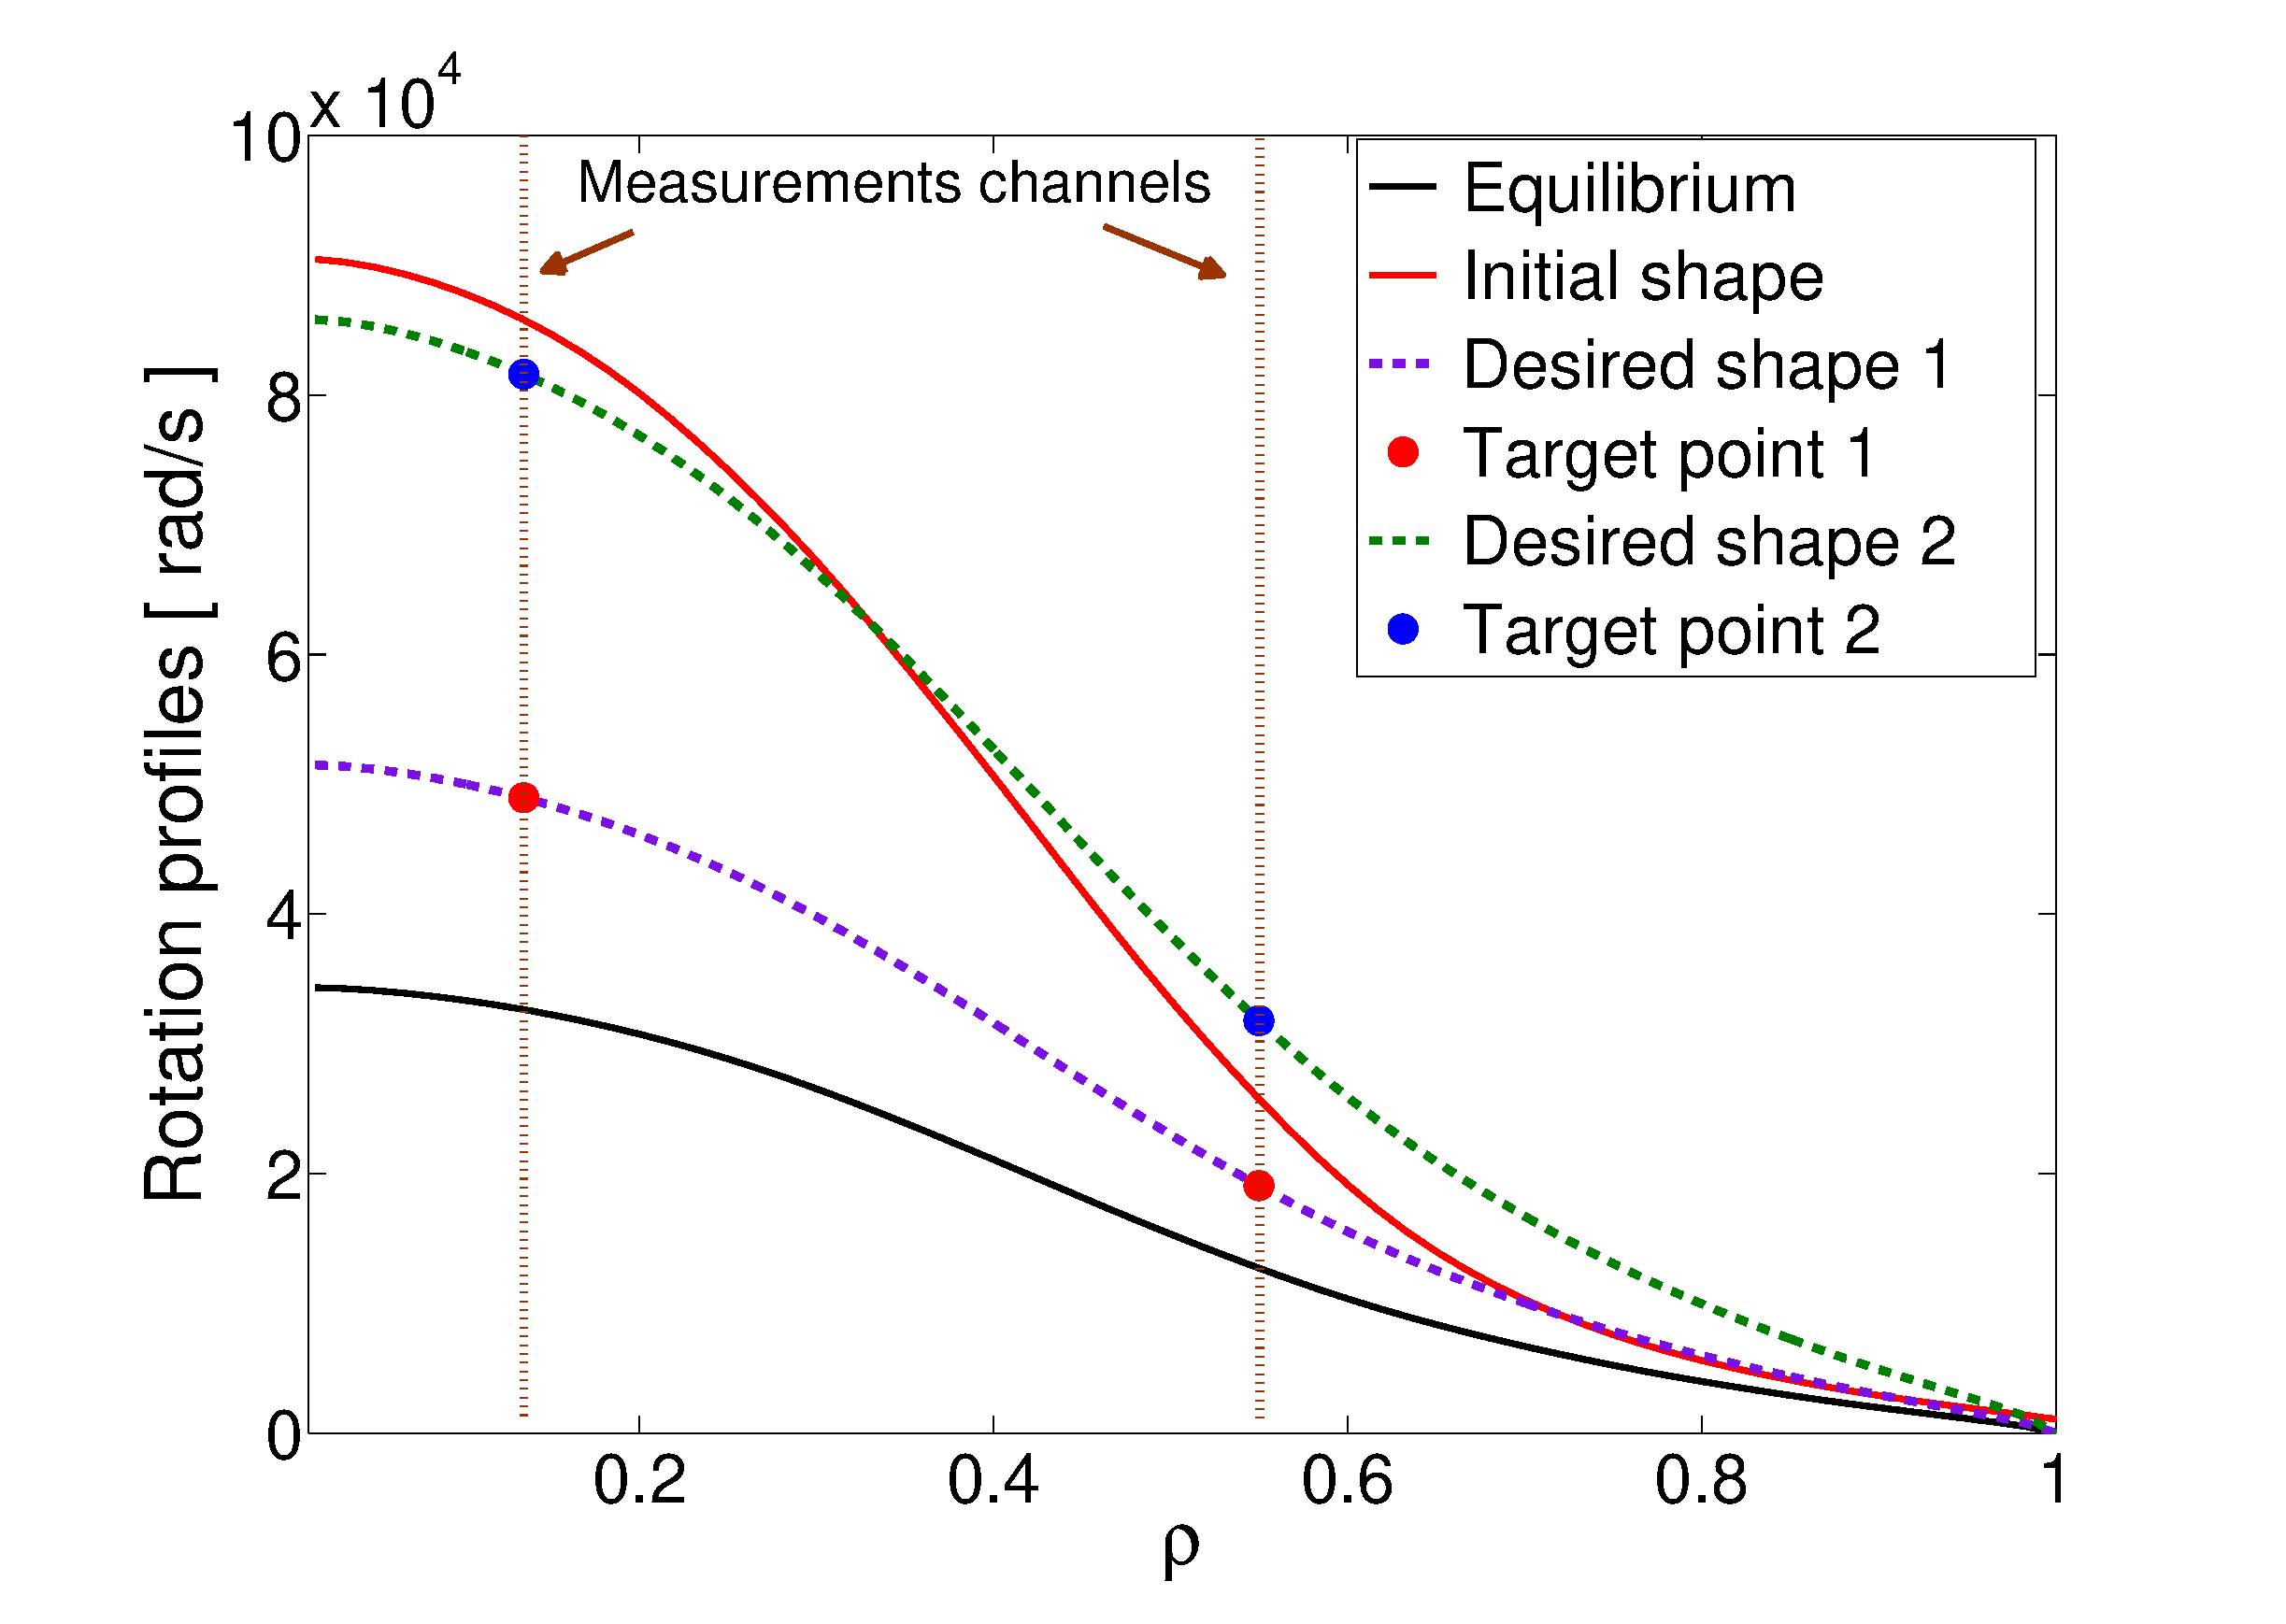
\includegraphics[width=\linewidth]{imene_figs/Goum133l}
\caption{Rotation profiles: definition of the initial profile, equilibrium profile $w_0$ used for the linearization and the desired profiles to reach $w_d$. The two points of measurement $r_d$ are shown by the two dots.}
\label{fig:rot11}
\end{figure}




\subsubsection{Observer-based feedback control design} 

In most applications, the state of the full system is unknown, and thus a full-state feedback controller that updates the control input based on the current state is not directly applicable. Instead, one typically uses an observer-based feedback controller to update the feedback control inputs based on the sensor measurements (outputs).
As done previously, and using the reduced-order model, an observer is designed using a Kalman filter as a quadratic estimator. This method is optimal if the errors in representing the reduced state $x_r$ and the measurements $y$ are stochastic Gaussian processes. 
Such errors typically arise from inaccuracies in the model, external disturbances, and sensor noise. For more details, see~\cite{SandP, AandM, Stengel}. 
Considering the state evolution equation as
\begin{eqnarray}
 \dot{\hat{x}}_1 &=  A \hat{x}_1 + B u_{1} + L (y_1 - C \hat{x}_1) =   (A- L C) \hat{x}_1 + B u_{1} + L y_1,
 \label{obs}
\end{eqnarray}
 where $L$ is the gain designed using a Kalman filter.    
The observer generates an estimate of the state from the physics model as represented by the state matrix, the inputs and outputs, and once combined to the feedback controller it forms a linear quadratic Gaussian compensator.
By plugging in equation~(\ref{eqn:ctrllaw_ff}) into equation~(\ref{obs}), we obtain after simplification
\begin{eqnarray}
      \dot{\hat{x}}_1 &=  (A- B K  -L C) \hat{x}_1 + B F r_{1d} + L y_1.
\end{eqnarray}


\subsubsection{Integrator, actuators saturation and anti-windup design} 

Because the primary goal is tracking the desired rotation profile, we want to minimize the steady state error between the output (measured) and the target profile. One way to handle such issue is to use integral action
\begin{eqnarray}
\dot{x}_i = y_1 - r_{1d} = C x_1 - r_{1d}.
 \label{integral}
\end{eqnarray}
The overall system can be then written as
\begin{equation}
\frac{\partial}{\partial t}   \left[\! \begin{array}{c}  x_1 \\ x_i\end{array}\!\right]
  ={ \left(\! \begin{array}{cc} A  & 0 \\ C & 0 \end{array} \! \right)} \left[\! \begin{array}{c} x_1 \\ x_i    \end{array}  \!\right] + \left(\! \begin{array}{c} B   \\ 0    \end{array}  \!\right) u_1 -  \left(\! \begin{array}{c}  0 \\ I \end{array}\!\right) r_{1d}
\label{int2}
\end{equation}
with a new feedback law designed as
\begin{equation}
u_1 =   - \left(\! \begin{array}{cc}  K & K_i\end{array}\!\right) \left[\! \begin{array}{c}  x_1 \\ x_i\end{array}\!\right] + F r_{1d}
\end{equation}
where the gains $K$ and $K_i$ can be determined through the MATLAB command LQI.\\

However, actuator saturation is a problem that occurs in control systems where the plant inputs are limited by maximum and or minimum allowable values. Thus the relation between the desired plant input and the actual plant input is modeled similarly to Figure~\ref{fig:saturation}
where $u_H$ and $u_L$ represent respectively, the maximum and minimum control effort allowed by the physical actuators.

\begin{figure}
	\centering
\begin{tikzpicture}[>=latex]
		\draw[->] (-5,0) -- (5,0) node[below] {$u_{req}$};
		\draw[->] (0,-3) -- (0,3) node[right] {$u_{actual}$};
		\draw (-0.1,-2) -- (0.1,-2) node[right] {$u_L$};
		\draw (-0.1,2) -- (0.1,2) node[right] {$u_H$};
		\draw[thick] (-5,-2) -- (-2,-2) -- (2,2) -- (5,2);
	\end{tikzpicture}
\caption{Actuator saturation function.}
\label{fig:saturation}
\end{figure}

Here in the case of the integrator with output $u_{req}$, everything is behaving well as long as $u_{req}$ is between $u_L$ and $u_H$. However if $u_{req}$ exceeds $u_H$, then $u_{actual}$ is limited to its maximum value $u_H$. This in itself may not be a problem. The problem arises if the steady state error remains positive, for then, the integrator continues to integrate and $u_{req}$ may increase well beyond $u_H$. Then when the steady state error becomes negative, it may take considerable time for $u_{req}$ to decrease below $u_H$. In the meantime, $u_{actual}$ is held at $u_H$, giving the incorrect control input to the system.
This effect of saturation is called the windup. It arises because the controllers we design are dynamical in nature, which means that they store energy and information. In order to correct for this, a common approach is to limit the state of the integrator so that it is consistent with the saturation effects being experienced by the plant input $u_{actual}$.

Compensating for windup consists of introducing a decay rate for $x_i$ tuned so that it is slow enough not to interfere with the dynamics but fast enough to prevent windup.
More details can be found in \cite{Lewis}

Once all different parts of the controller are defined, handled and designed, all one is left with is to combine them all into a global controller that contains all the characteristics and aspects of the dynamics.
Figure~\ref{fig:model1} shows the schematic of this general controller that combine the LQR, the observer, the integrator and the anti-windup detailed above.

\begin{figure}
\begin{tikzpicture}[x=0.75cm]
		\node (r) {$r_{1d}$};
		\node[junction, right=1.5 of r] (r in) {};
		\node[block, right=2 of r in] (N) {$N$};
		\node[block, below=of N] (L) {L};
		\node[sum, right=of L] (sum feedback) {};
		\node[block, right=0.9 of sum feedback] (K) {$K$};
		\node[sum, right=5 of N, yshift=3] (sum inputs) {};
		\node[junction, right=1 of sum inputs] (before sat) {};
		\node[block, right=0.5 of before sat] (sat) {
			\begin{tikzpicture}
				\draw[very thin] (-.4,0) -- (.4,0) (0,-.25) -- (0,.25);
				\draw[very thick] (-.4,-.2) -- (-.2,-.2) -- (.2,.2) -- (.4,.2);
			\end{tikzpicture}
		};
		\node[junction, right=0.5 of sat] (after sat) {};
		\node[block, right=1.5 of after sat] (P) {Plant};
		\node[junction, right=0.7 of P] (P out) {};
		\node[right=0.7 of P out] (y) {$y_1$};
		\node[junction, left=1 of L, yshift=3] (y in) {};
		\node[coord, left=1 of L, yshift=-3] (sub y in) {};
		\node[coord, label=left:$y_1$, left=2.4 of y in] (y input) {};
		\node[block, above=of N] (Ki) {$K_i$};
		\node[sum] (sum lqi) at (Ki -| y in) {};
		\node[sum, right=of Ki] (AW out) {};
		\node[block, right=0.9 of AW out] (integrator) {$\displaystyle\int$};
		\node[sum, above=0.5 of sat] (sum AW) {};
		\node[block, above=0.5 of sum AW] (AW) {AW};
		
		\draw[connector] (r) to (r in) to (N);
		\draw[connector] (N.east |- sum inputs) to node [above] {$u_{1d}$} (sum inputs);
		\draw[connector] (N)[yshift=-12] -| node [right, near end] {$x_{1d}$} (sum feedback);
		\draw[connector] (sum feedback) to (K);
		\draw[connector] (K) -| (sum inputs);
		\draw[connector] (sum inputs) to (before sat) to (sat);
		\draw[connector] (sat) to (after sat) to ++(down:2.6) -| (sub y in) to (sub y in -| L.west);
		\draw[connector] (after sat) to node [above, pos=0.7] {$u_1$} (P);
		\draw[connector] (P) to (P out) to (y);
		\draw[connector] (P out) -- ++(down:3.5) -| (y input) to (y in) to (y in -| L.west);
		\draw[connector] (L) to node [above] {$\hat x_1$} node [below, very near end] {$-$} (sum feedback);
		\draw[connector] (r in) |- node [above, very near end] {$-$} (sum lqi);
		\draw[connector] (y in) to (sum lqi);
		\draw[connector] (sum lqi) to (Ki);
		\draw[connector] (Ki) to (AW out);
		\draw[connector] (AW out) to (integrator);
		\draw[connector] (integrator) -| node [right, pos=0.95] {$-$} (sum inputs);
		\draw[connector] (before sat) |- (sum AW);
		\draw[connector] (after sat) |- (sum AW);
		\draw[connector] (sum AW) to (AW);
		\draw[connector] (AW) to ++(up:0.6) -| (AW out);
		
		\draw[green!50!black, ultra thick] (1.4,-2.8) rectangle (15.6,3.1);
		\node[green!50!black, anchor=south, font=\large\bfseries] at (8.4,3.1) {Controller};
	\end{tikzpicture}

\caption{Global schematic of the controller that combine a feedforward $(N)$, a LQR $(K)$, an observer $(L)$, an integrator $(K_i)$ and an anti-windup $(AW)$.}
\label{fig:model1}
\end{figure}


\clearpage


\section{Simulation results} 
The goal of the simulations is to test the controller first on the simplified reduced-order model, then try a closed loop simulation on a more complex model (TRANSP) which is closer to the experimental testing.  The desired profiles shown in Figure~\ref{fig:rot11} will be targeted in both cases and the results will be compared to see the effectiveness of the controller described above.

\subsection{Actuator constraints}
\label{constraints}

Both actuators (NTV coil current and NBI beam power) have constraints that need to be satisfied when applied on the real device (NSTX). Some of these constraints are made for the safety of the operations, some of them reflect the practicability and the feasibility of some requests to the device. The controller will mimic some of these constraints which will be added to the dynamics equations.

The coil current will be constrained between 0 and 3000 amperes.
The coil current response is fast compared to the dynamics of the system that it can be assumed to be applied instantaneously.

Although we have so far been treating the NBI actuator as a single source outputting between 2 and 6\,MW of power, it is actually composed of 3 beams. Each beam can either be ON and produce 2\,MW of power or OFF and produce 0\,MW.
In addition, each beam can only be switched ON or OFF a maximum of 20 times per plasma discharge to prevent device fatigue issues, and there is a refractory period of 10\,ms after each switch during which the beam cannot be switched again.
Due to diagnostic considerations, one NBI source is typically always on, and so the overall injected power is considered to be between $2$ and $6$ MW here.

These physical restrictions constrain the model and controller to be discrete and to use Pulse Width Modulation (PWM) for the beam power actuation in order to obtain control requested values between 2 and 6\,MW.


\subsection{Simulation without PWM}
\label{noPWM}

The discretized controller is first applied to the reduced-order model, considering only the constraint of saturation for both actuators. It is thus considered that any values of beam power between $2$ and $6$\,MW and coil current between $0$ and $3000$\,Amps can be applied instantaneously.   

\begin{figure}
\begin{tabular}{cc}
$t = 0.50 s$  & $t = 0.51 s$ \\
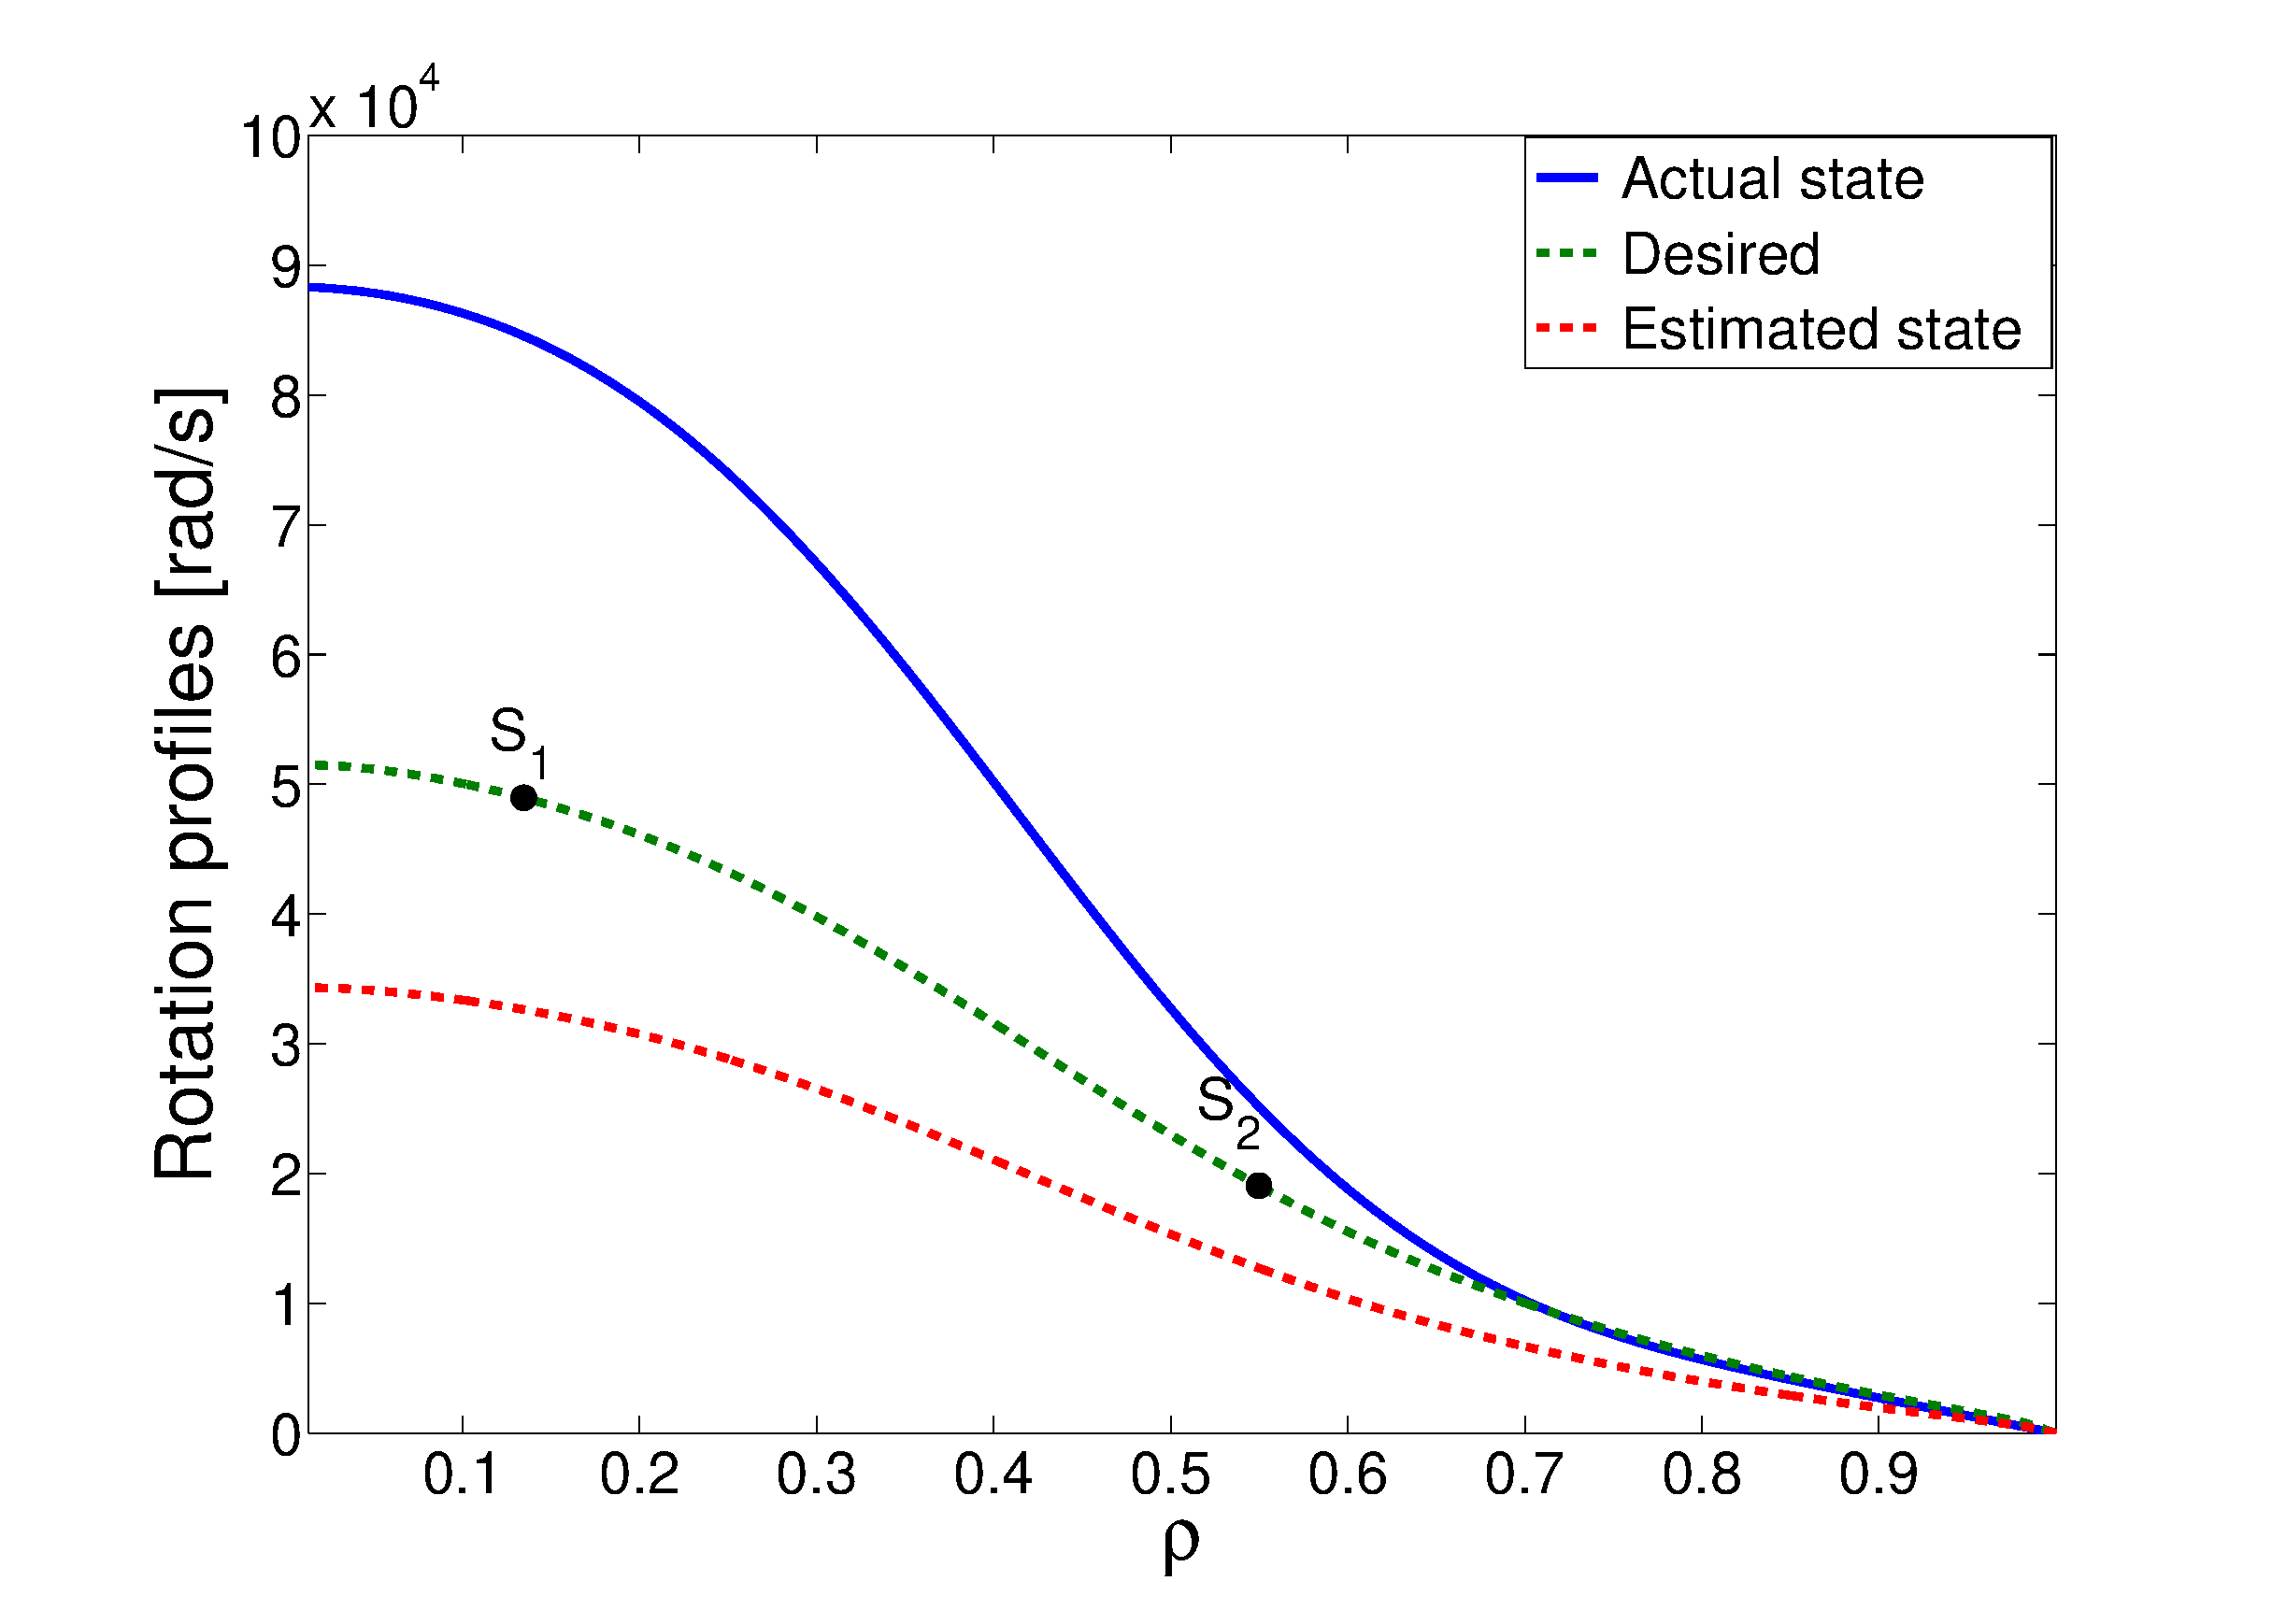
\includegraphics[width=0.5\linewidth]{imene_figs/Goum18lnn} & 
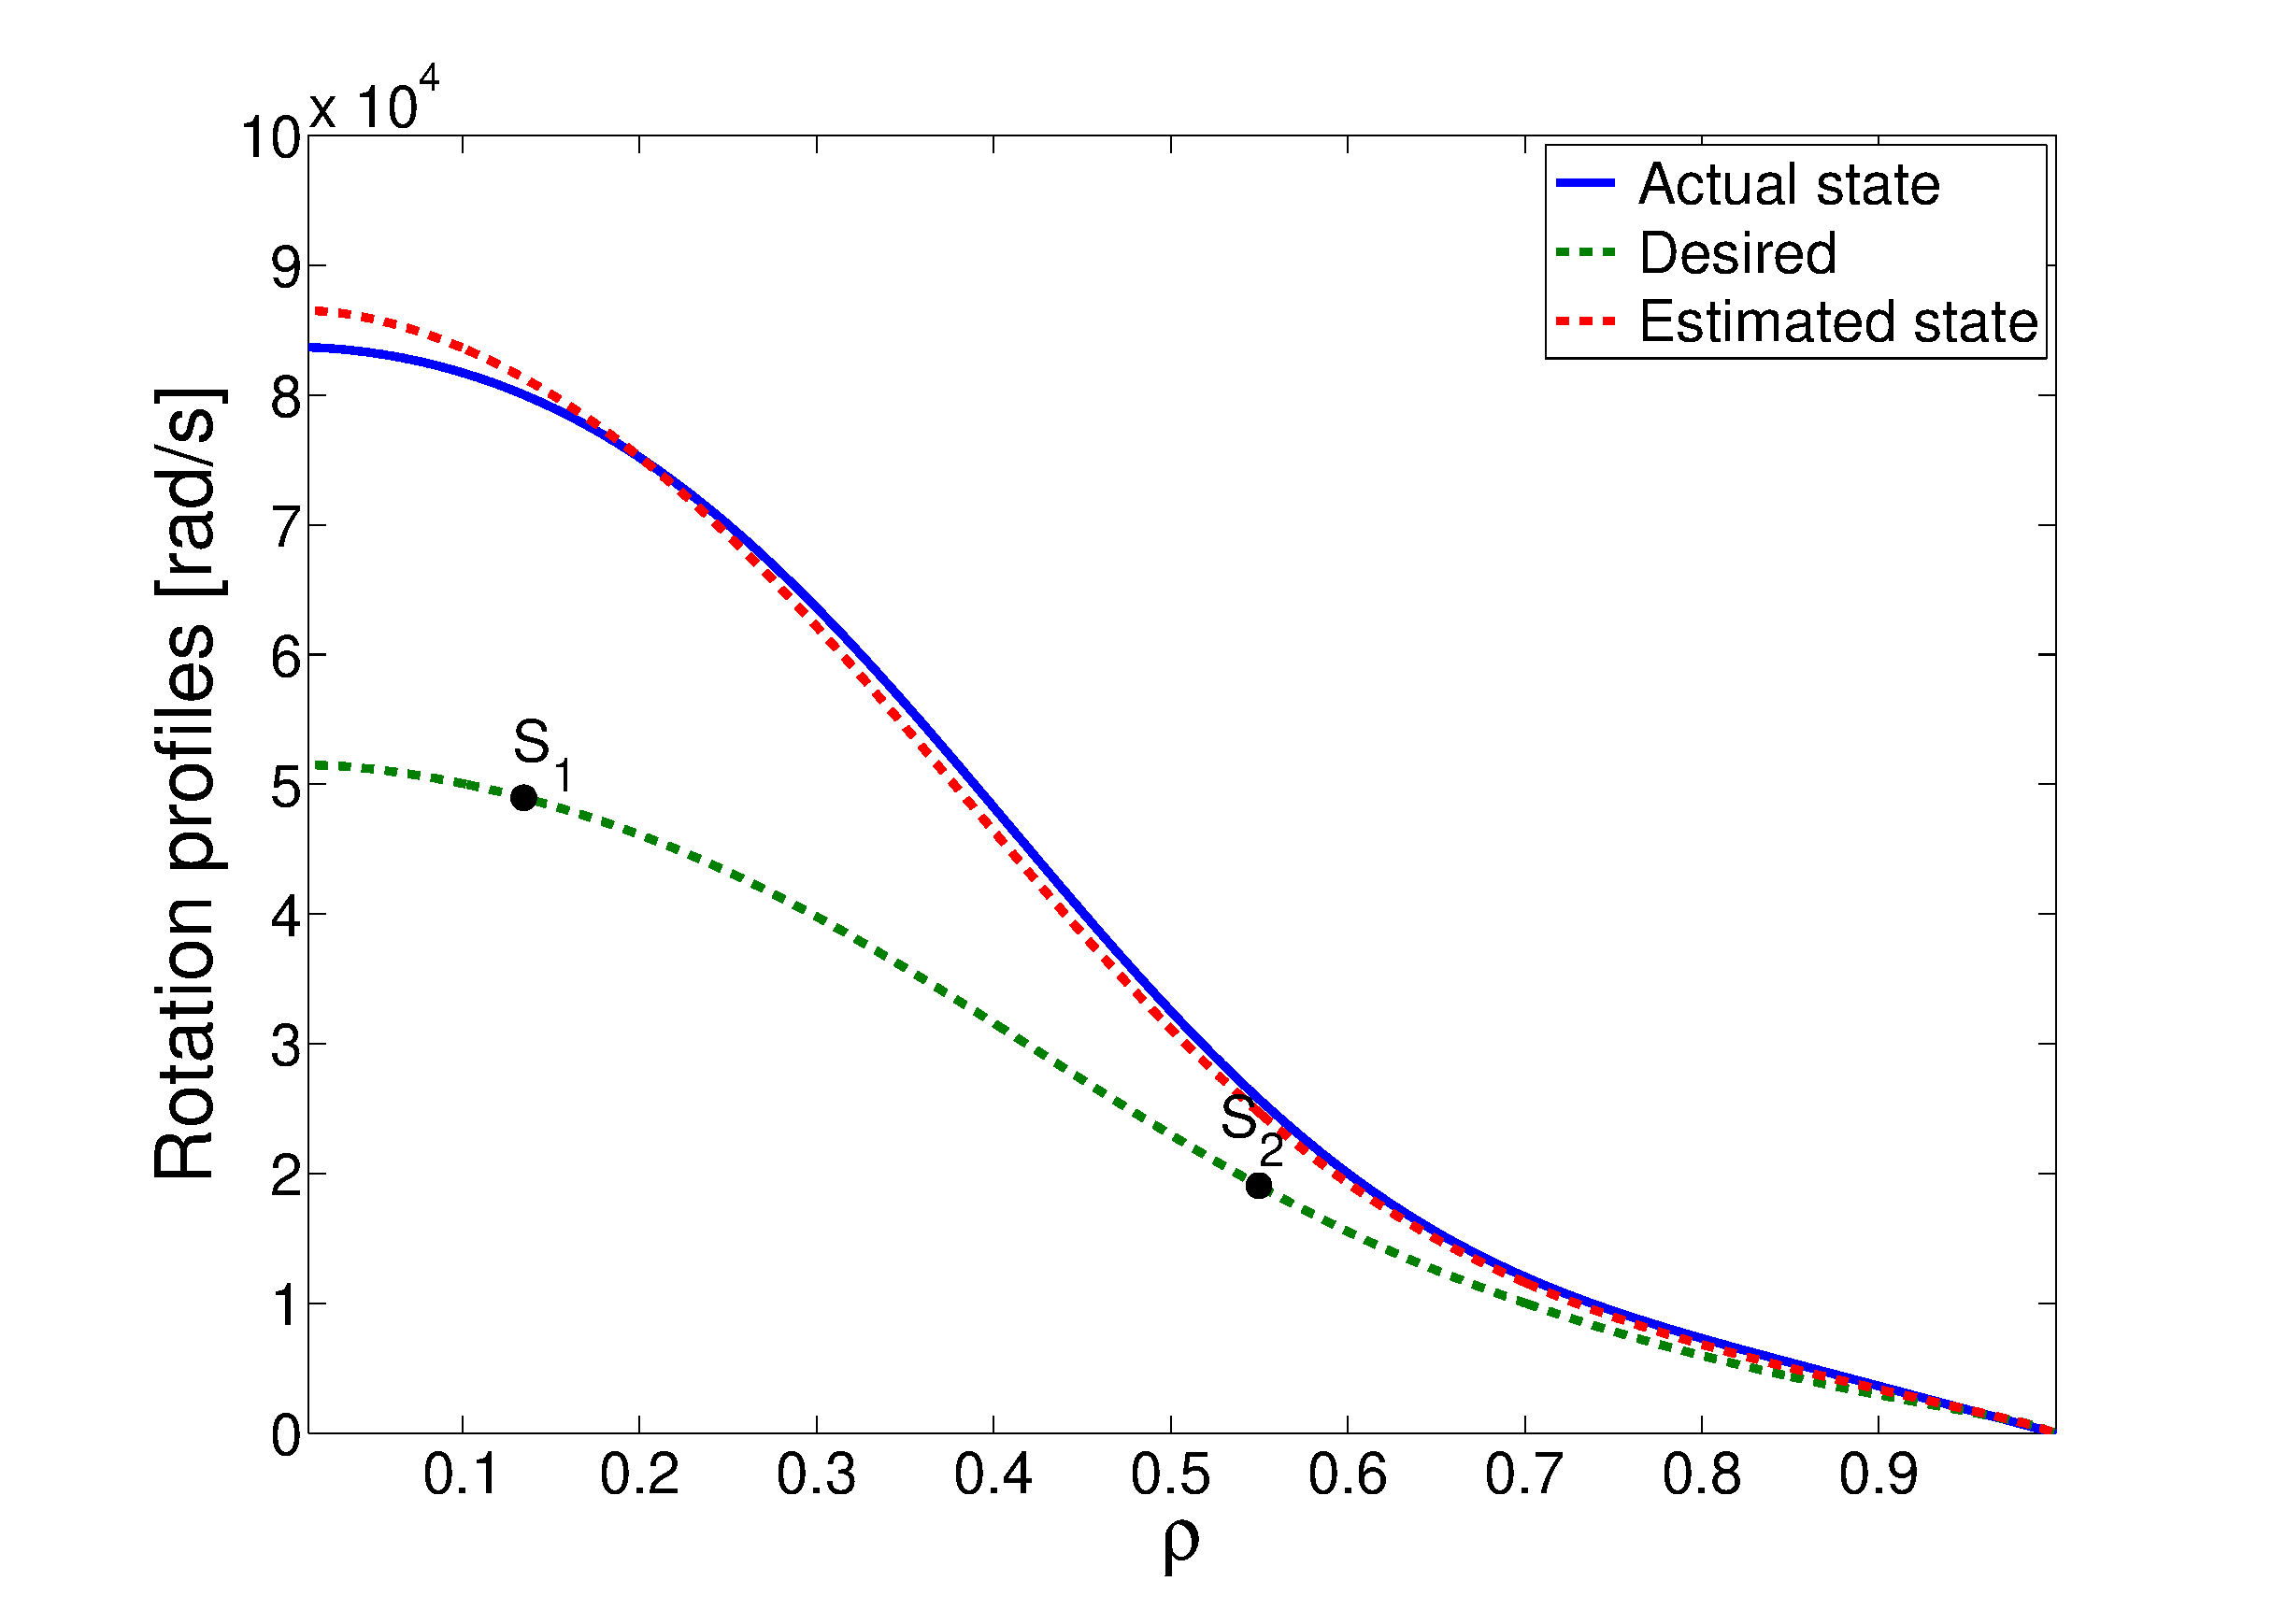
\includegraphics[width= 0.5\linewidth]{imene_figs/Goum18lln} \\ 
$t = 0.52 s$  & $t = 0.57 s$ \\
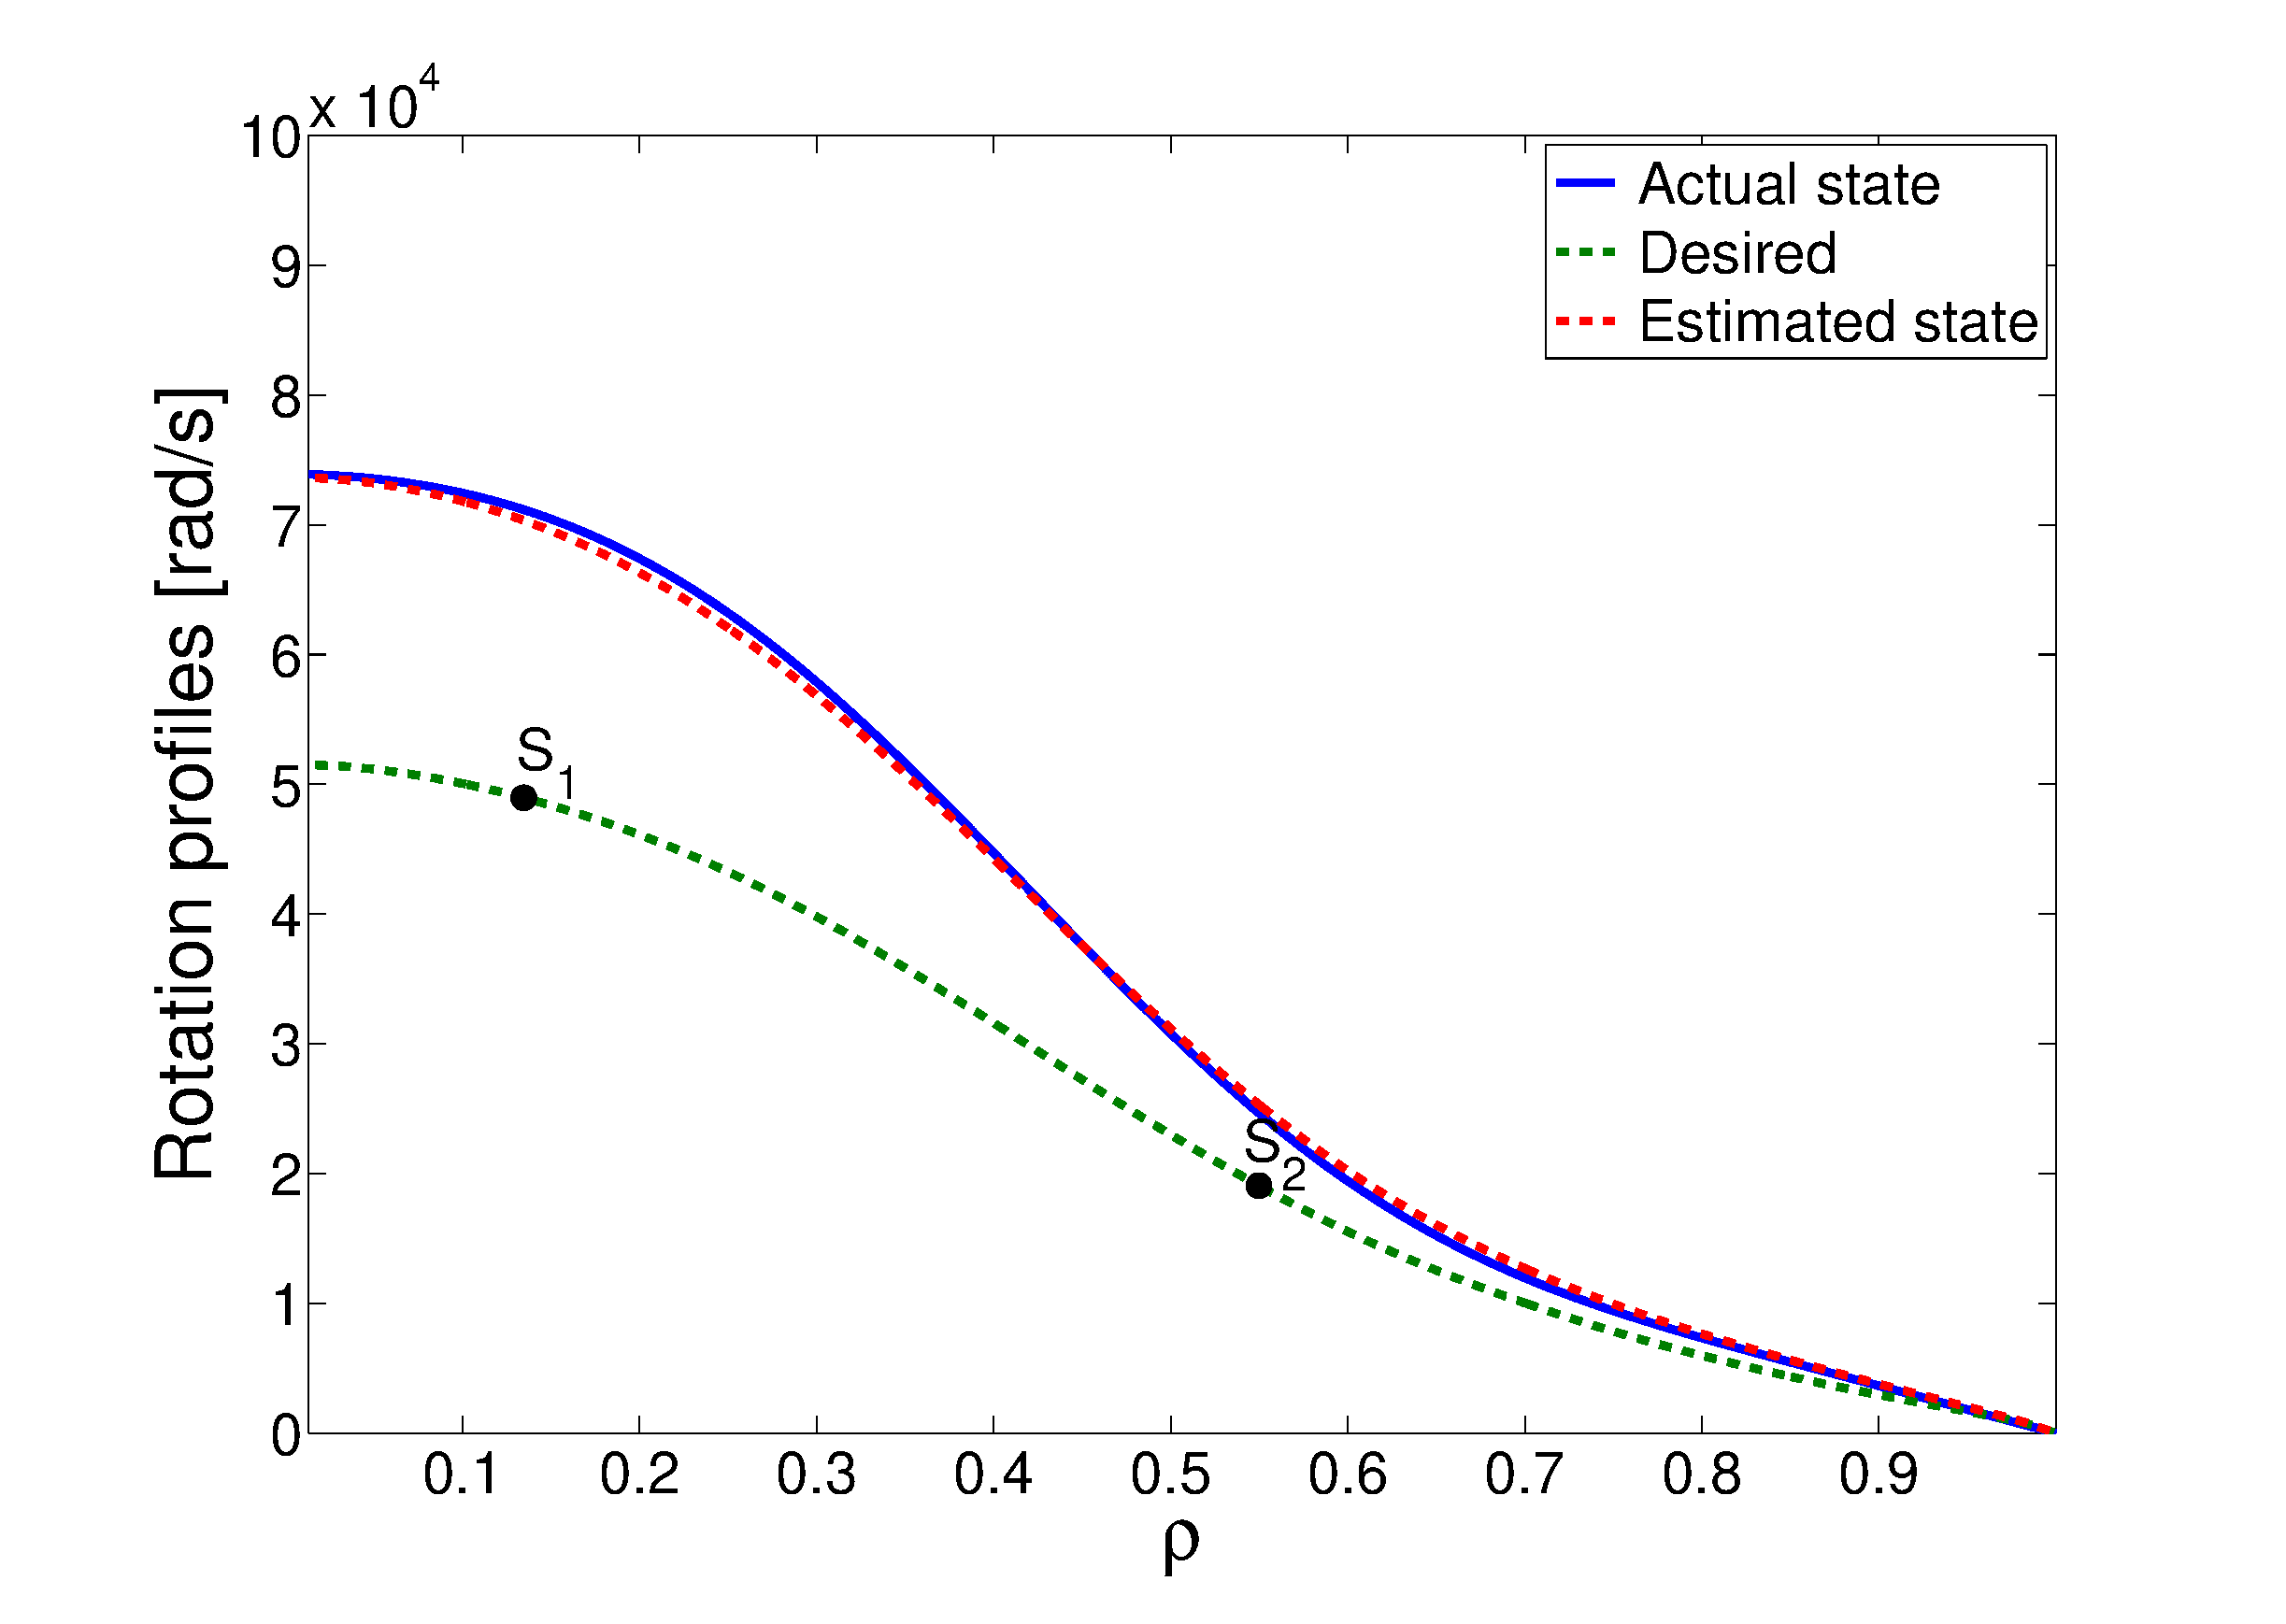
\includegraphics[width=0.5\linewidth]{imene_figs/Goum18llln} &
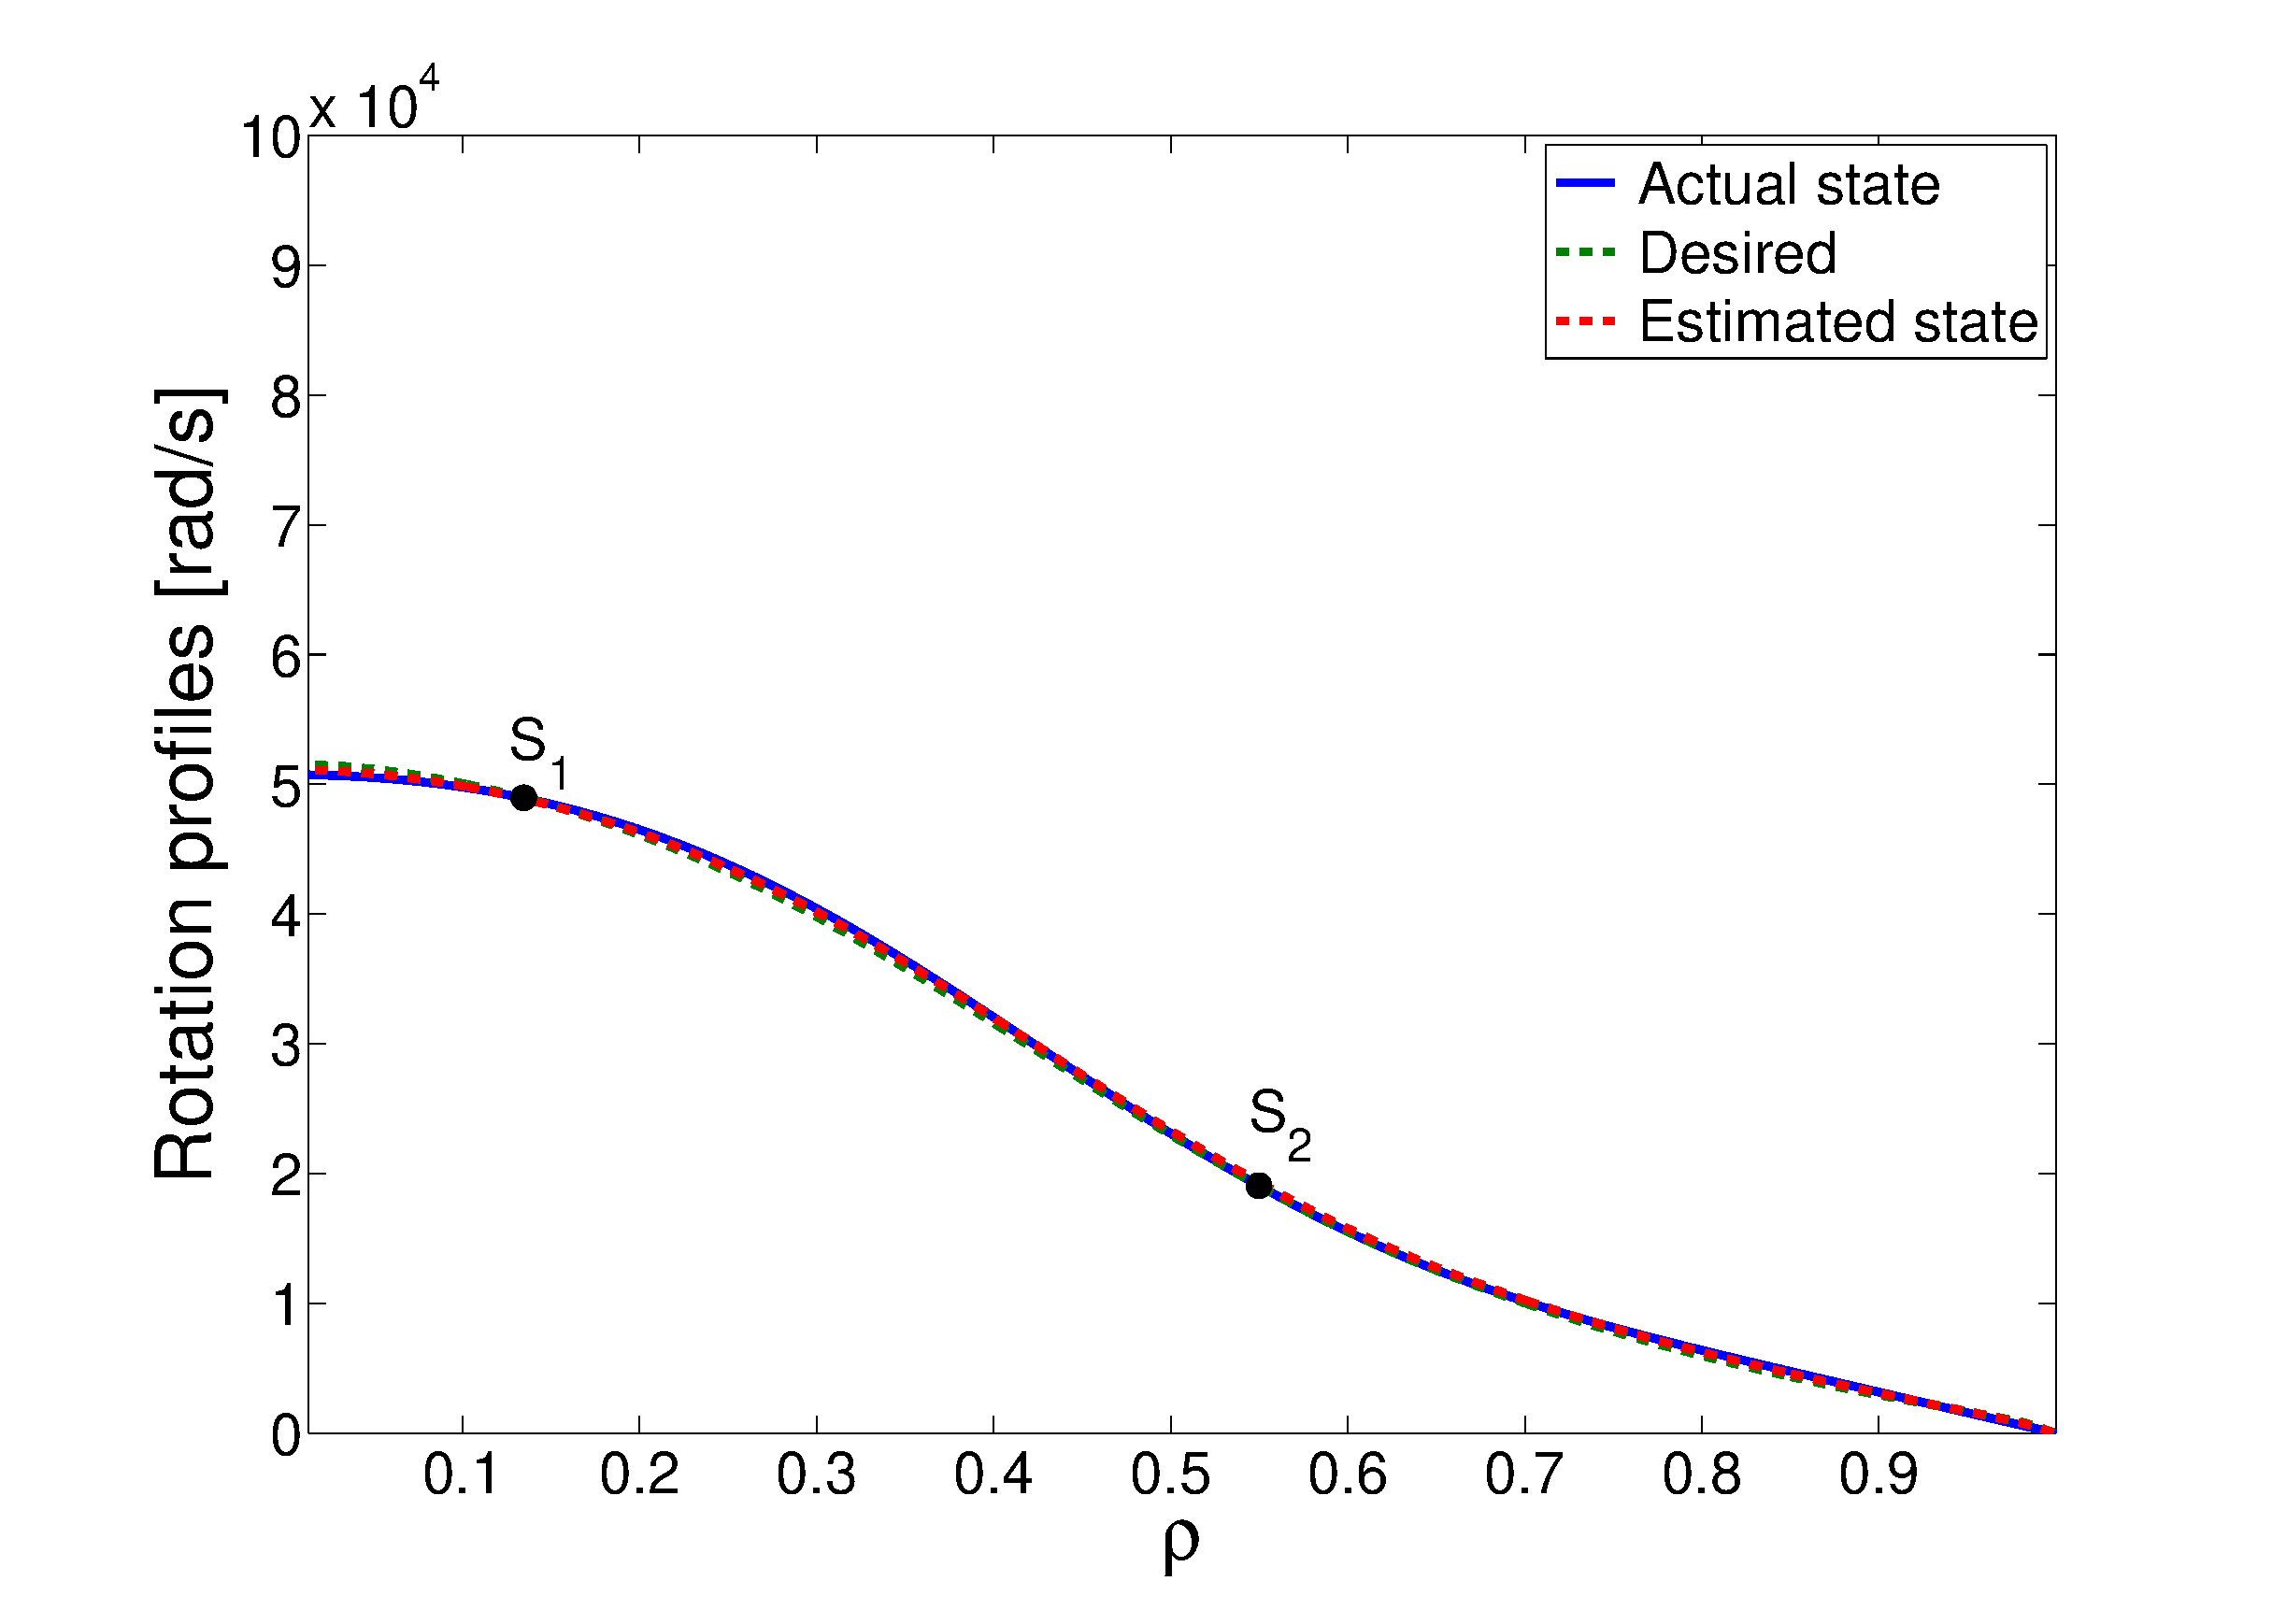
\includegraphics[width=0.5\linewidth]{imene_figs/Goum18lllln} 
\end{tabular}
\caption{Time evolution of the rotation in the model as it evolves toward the target values and its estimate at 4 different times. The green profile is the targeted rotation profile. }
\label{fig:rot18}
\end{figure}


Figure~\ref{fig:rot18} represents the time evolution of the rotation in the model as it evolves toward the target values and its estimate (from the observer) at 4 different times: $0.5$\,s (Controller ON), $0.51$\,s, $0.52$\,s and $0.57$\,s respectively. it shows also where the two sensors are placed, and it can be noticed that the first targeted profile defined in Figure~\ref{fig:rot11} is reached in less than $0.1$\,s. The controller is applied on the reduced-order model at $0.5$\,s.
\begin{figure}
\centering
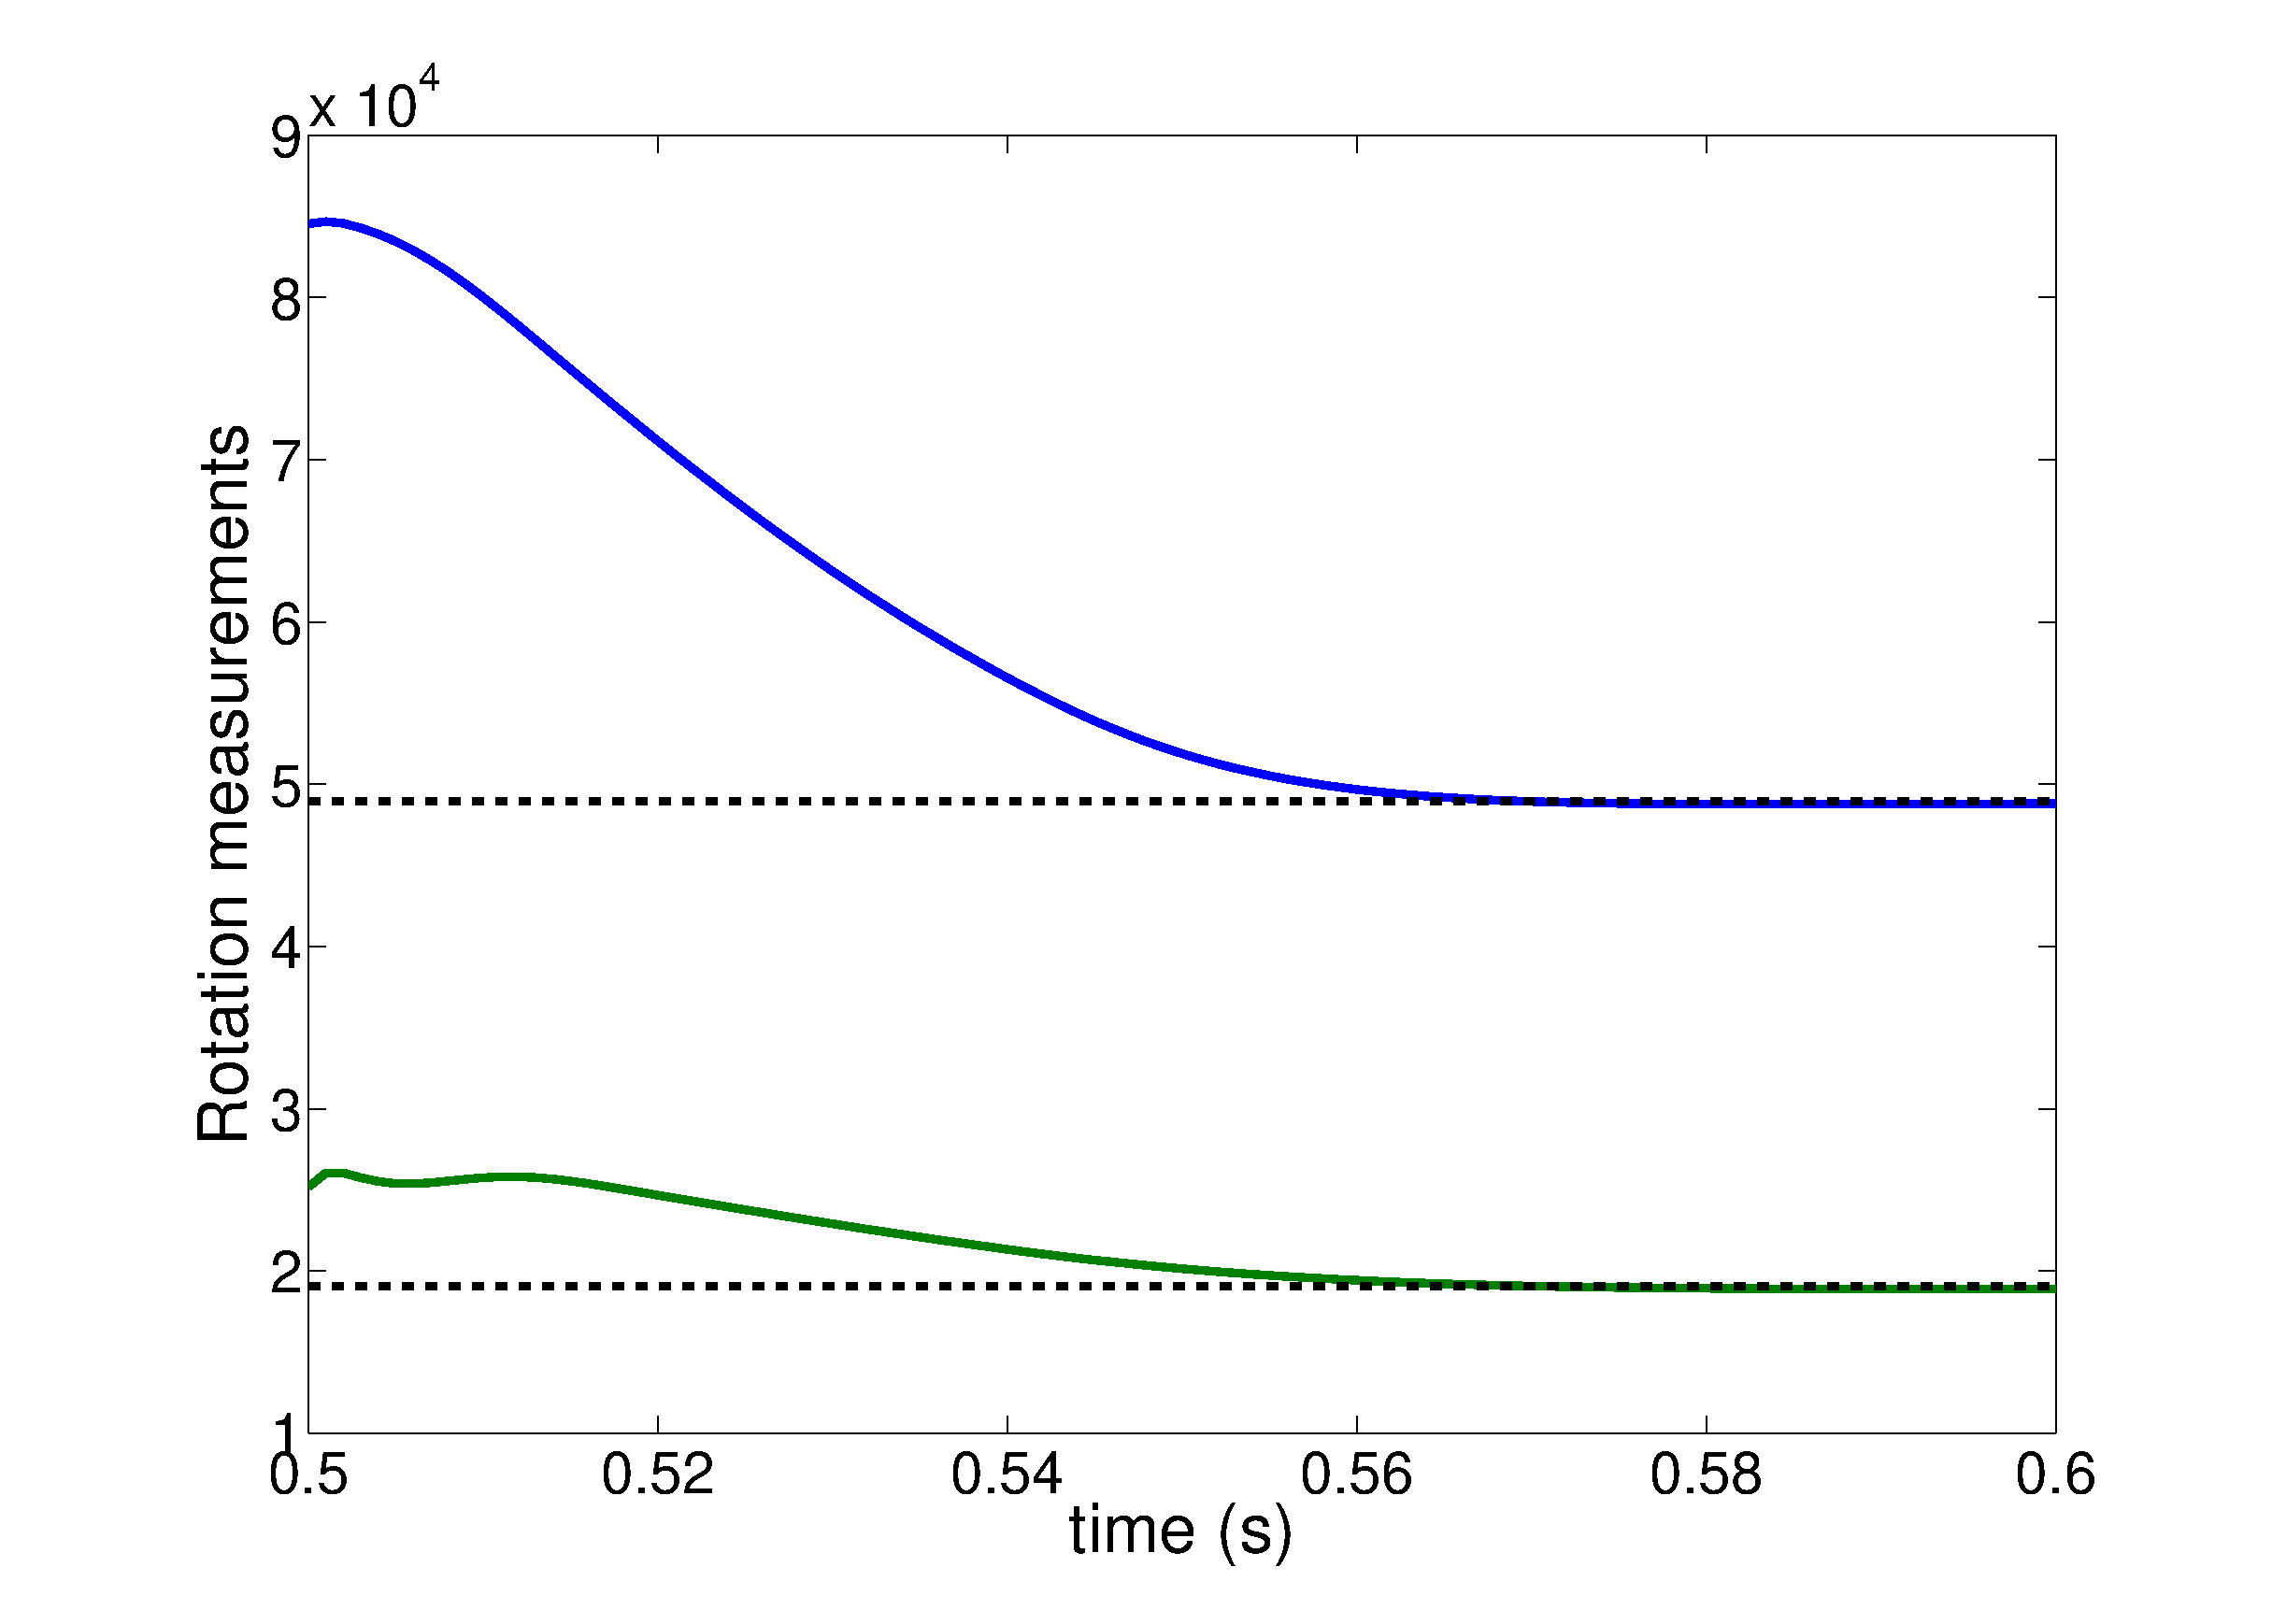
\includegraphics[width=\linewidth]{imene_figs/Goum20n} 
\caption{Time evolution of the rotation measurement at the two sensor points. The dashed lines represents the desired measurements at these latter locations. }
\label{fig:rot20}
\end{figure}    

Figure~\ref{fig:rot20} represents the time evolution of the rotation measurement at the two sensor points located at the core and towards the edge of the plasma respectively.  



\begin{figure}
\centering
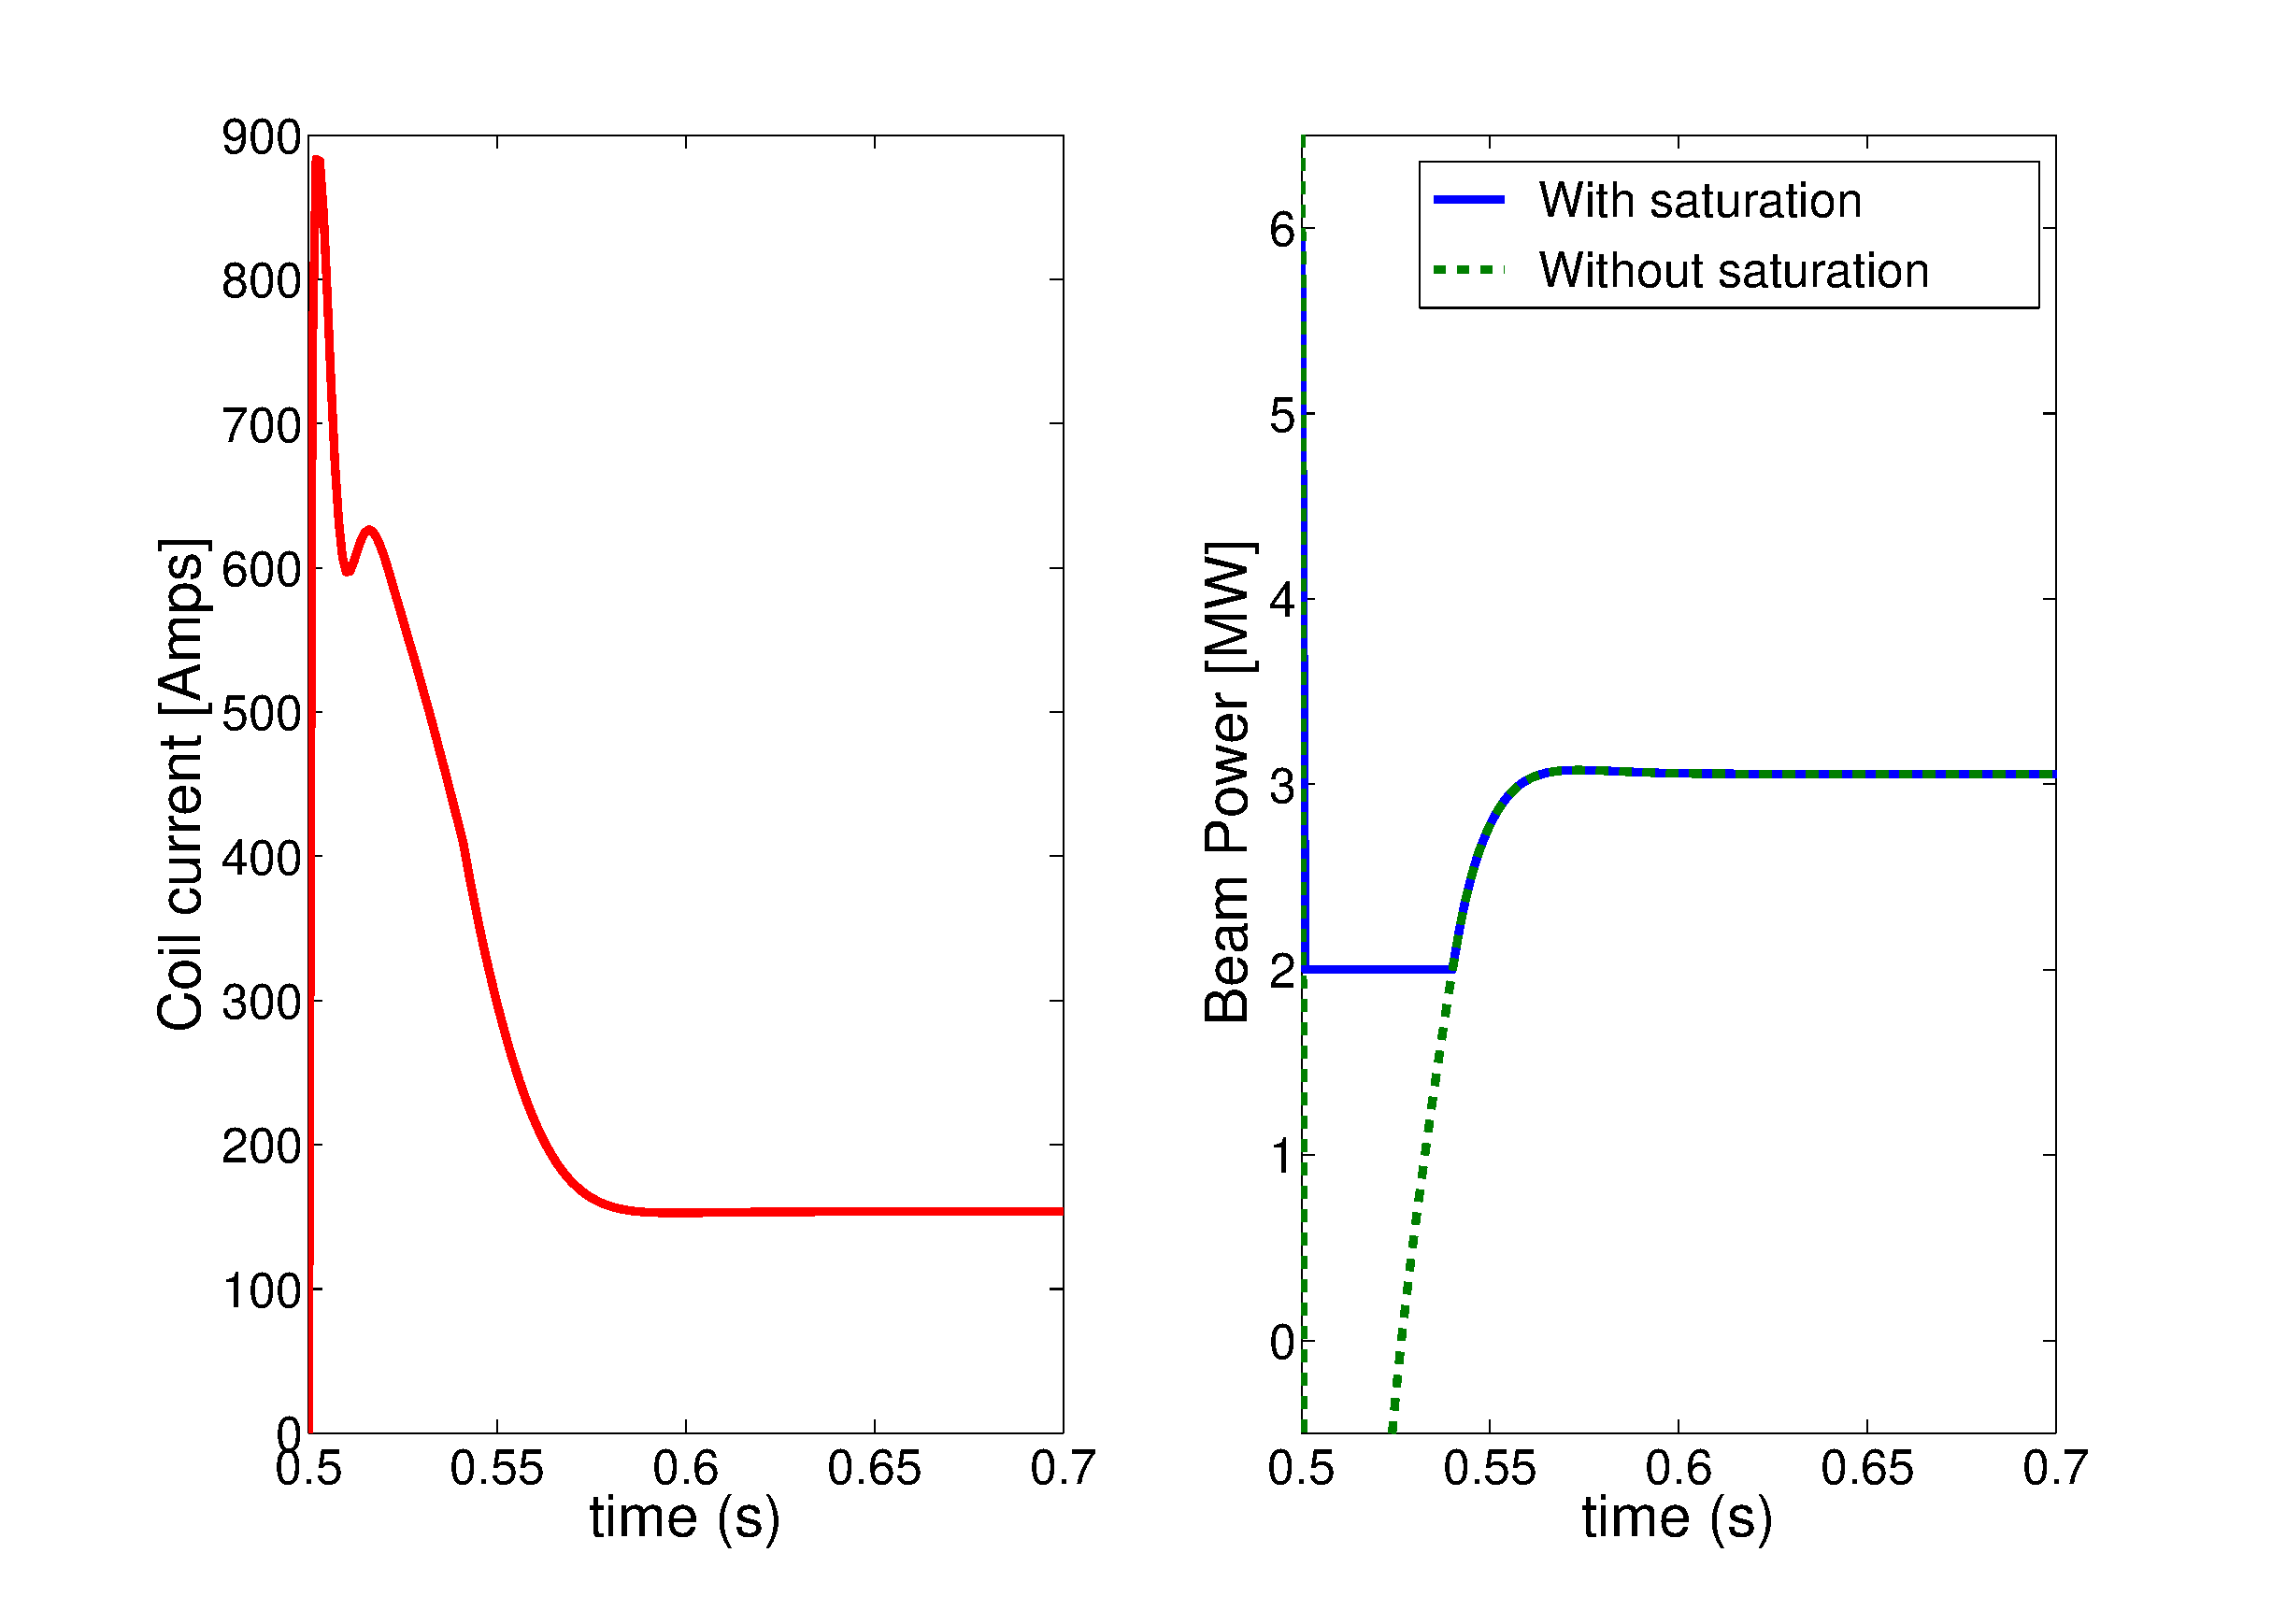
\includegraphics[width=\linewidth]{imene_figs/Goum19ln} 
\caption{Time evolution of the coil current and the overall beams power and its saturation, needed to reach the 1st desired profile }
\label{fig:rot19}
\end{figure} 

Figure~\ref{fig:rot19} represents the requested inputs (coil current and overall beam power) needed to reach the desired profile of Figure~\ref{fig:rot18}. It can be noticed that the current does not saturate whereas the beam power does.

Because the initial profile (profile \#(1) in Figure~\ref{fig:rot18}) before turning the controller ON, is above the targeted profile  (profile \#(4) in Figure~\ref{fig:rot18}), and the difference between the two profiles is higher towards the core of the plasma (where the beam power acts), the controller tries to first push the power down starting from $6$\,MW at the initial state before controlling, up to $2$\,MW when it hits saturation. The green dashed line in Figure~\ref{fig:rot19} shows how the controller would actuate the beam power if no saturation was effecting. During the rapid decrease of the beams power, the controller increases the coil current in order to increase the drag and allows a quicker descent action towards the edge of the desired profile.  
The controller and the actuators, when they can be activated instantaneously, enable the rotation profile to reach its target about 2 times faster (about 60 ms) compared to the momentum diffusion time (about 100 ms).

\subsection{Computational approach for TRANSP}
In order to predict the toroidal rotation for NSTX, the TRANSP code running in predictive mode is used for a given beam power and coil current. It also takes as inputs the time histories of the plasma boundary shape, plasma current, electron and ion (Chang-Hinton model \cite{Changhinton}) temperature and density profiles and the momentum diffusivity coefficient.

The actuator commands needed for closed-loop rotation control simulations are entered into the TRANSP code, which serves as a plasma simulator for testing the present controller. For more details on the TRANSP implementation, see \cite{Boyer15}.

\subsection{Simulation with PWM}
The discretized controller is now applied to the reduced-order model and the TRANSP predictive model, considering all the constraints listed in Section~\ref{constraints} for both actuators. The main difference with Section~\ref{noPWM} will be that instead of applying the exact beam power numerical value as requested by the controller, each of the 3 beams will be modulated individually while satisfying all the constraints.

At the beginning of each duty cycle, the controller sets the requested power. During the duty cycle, the beams switch ON and OFF at most once to minimize the number of switches. Because of this and the 10\,ms refractory period, the exact requested power cannot always be met.

To compare output results for different duty cycle durations, durations greater and smaller than 10\,ms are chosen. The longer the duty cycle, the better for the device because it means less commands switches so less fatigue, but a longer duration introduces a longer controller lag which impairs performance.
  
\begin{figure}
\centering
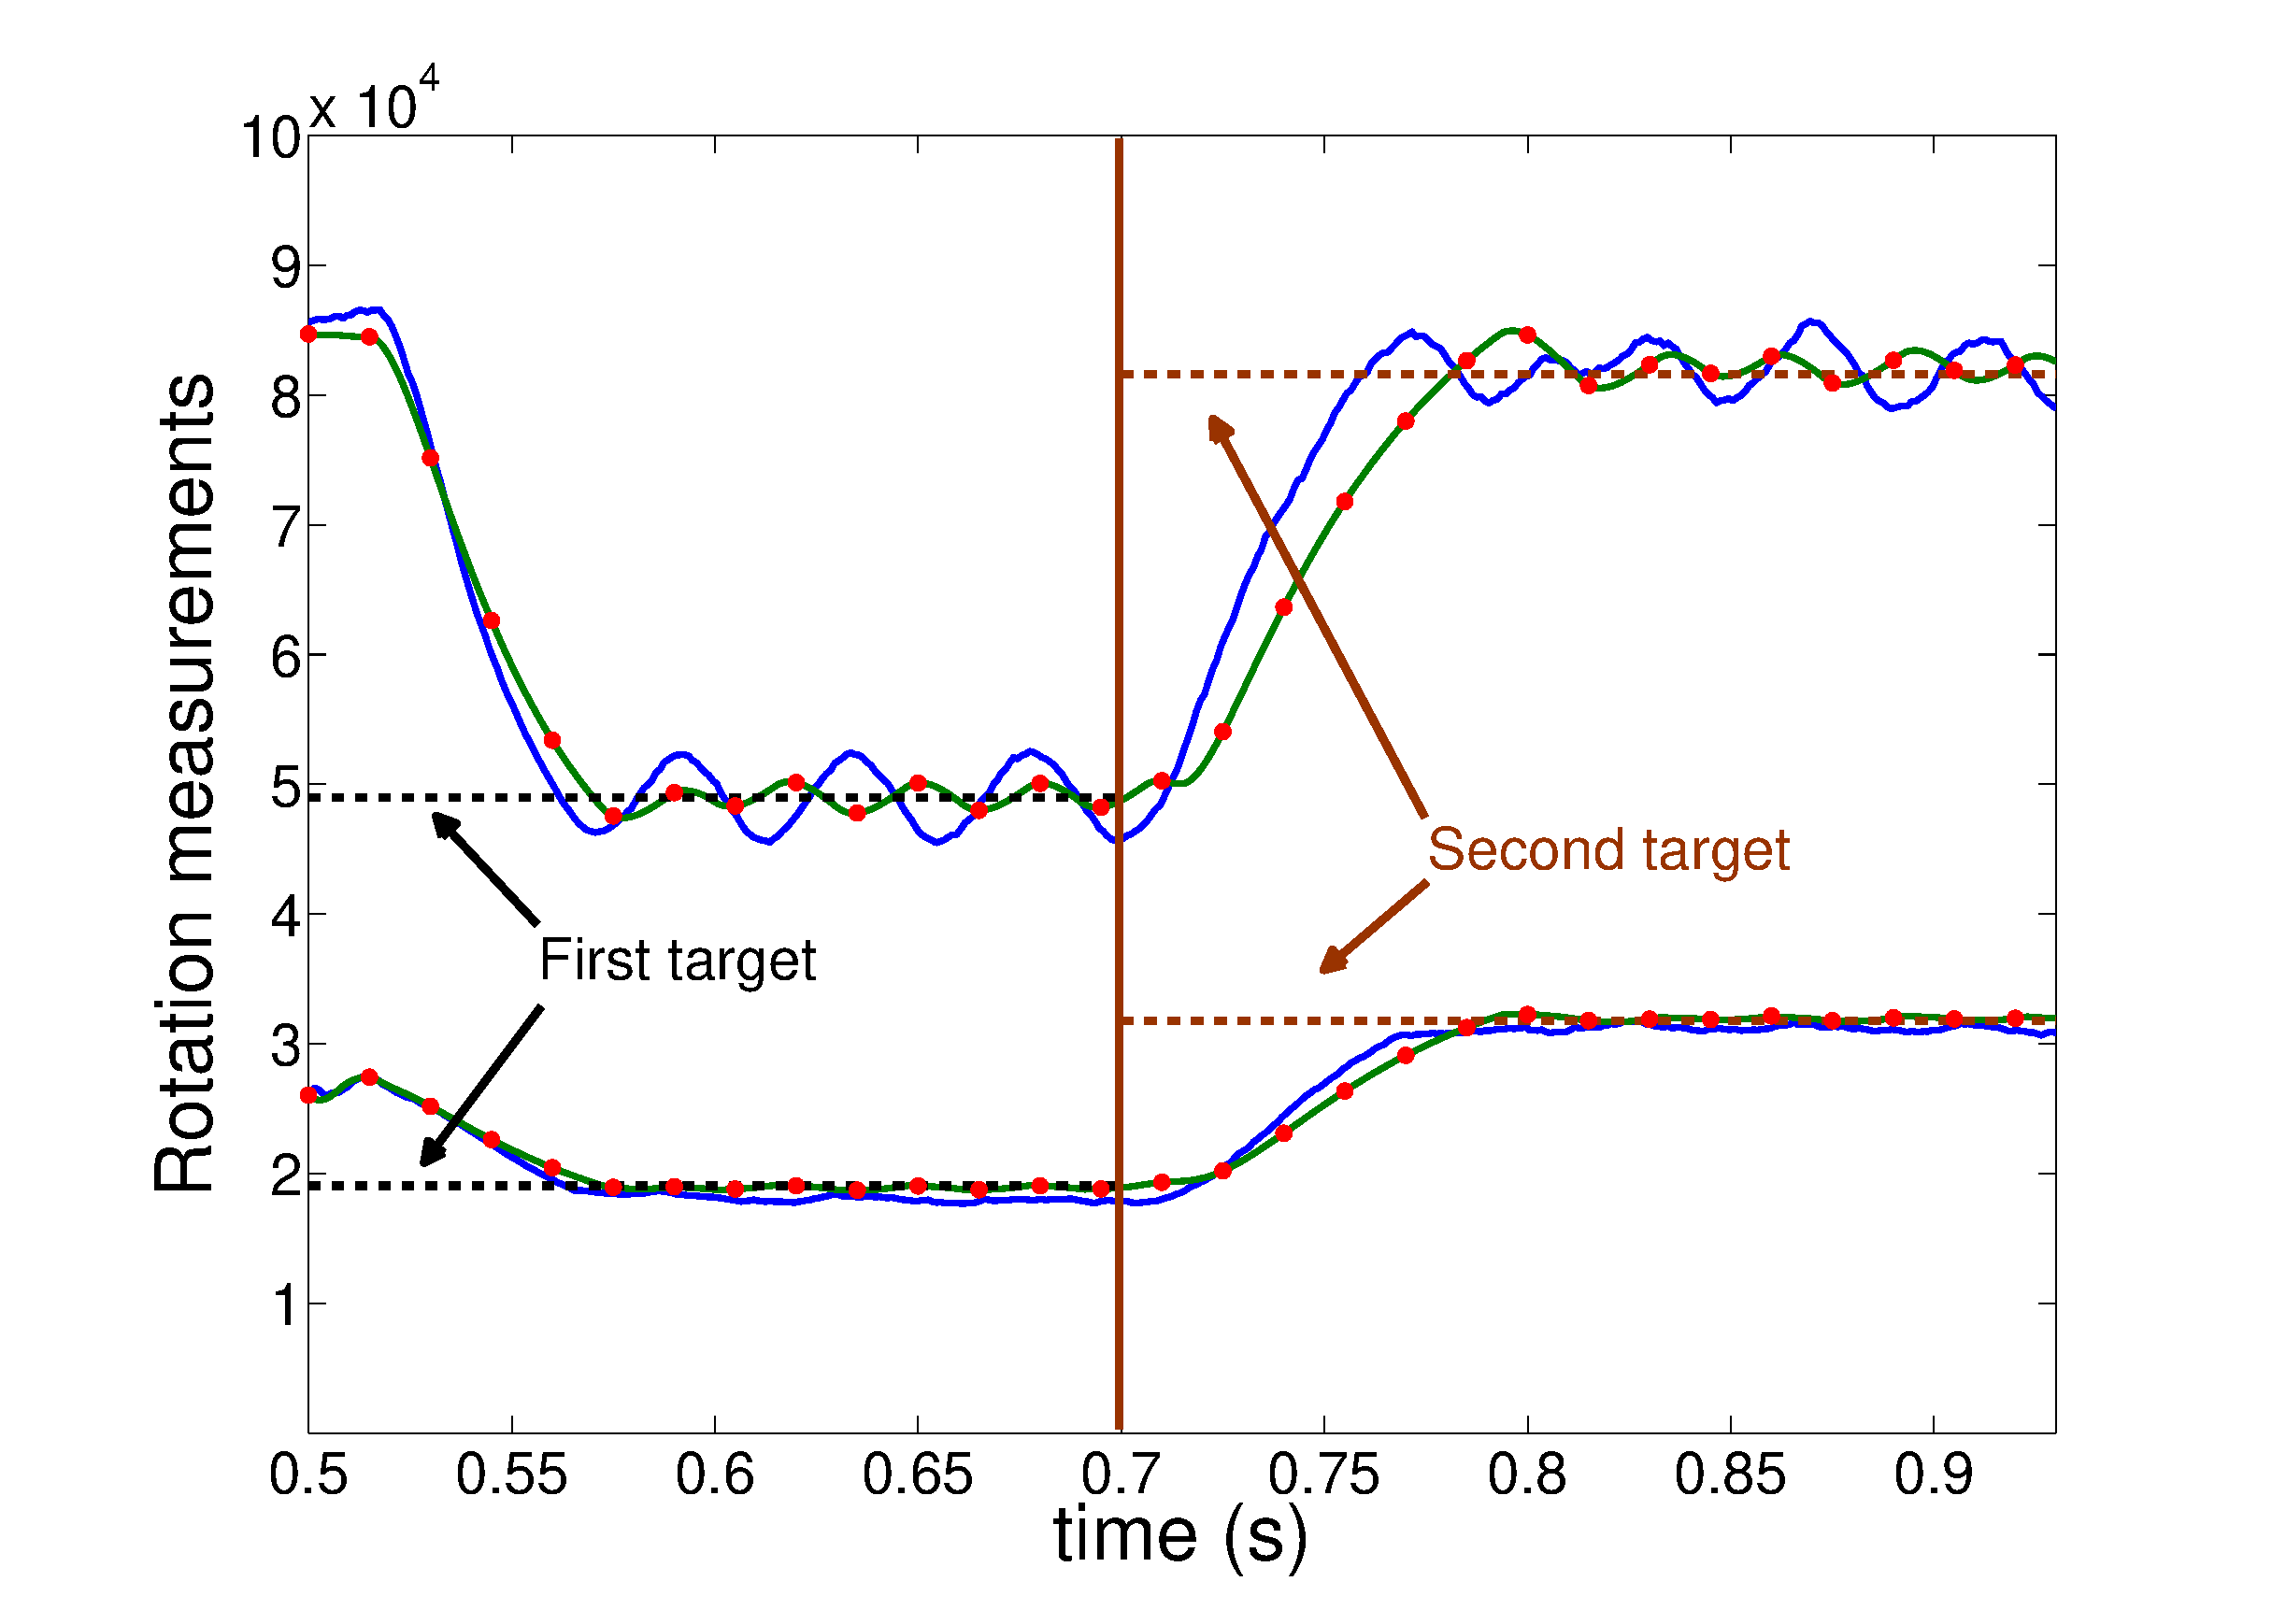
\includegraphics[width=\linewidth]{imene_figs/Goum14ln} 
\caption{Comparison of the rotation measurements when PWM is applied for both the reduced-order model (green lines) and the TRANSP predictive model (blue lines). The red dots represents the cycle times (every $0.015 s$).}
\label{fig:rot14}
\end{figure}

\begin{figure}
\centering
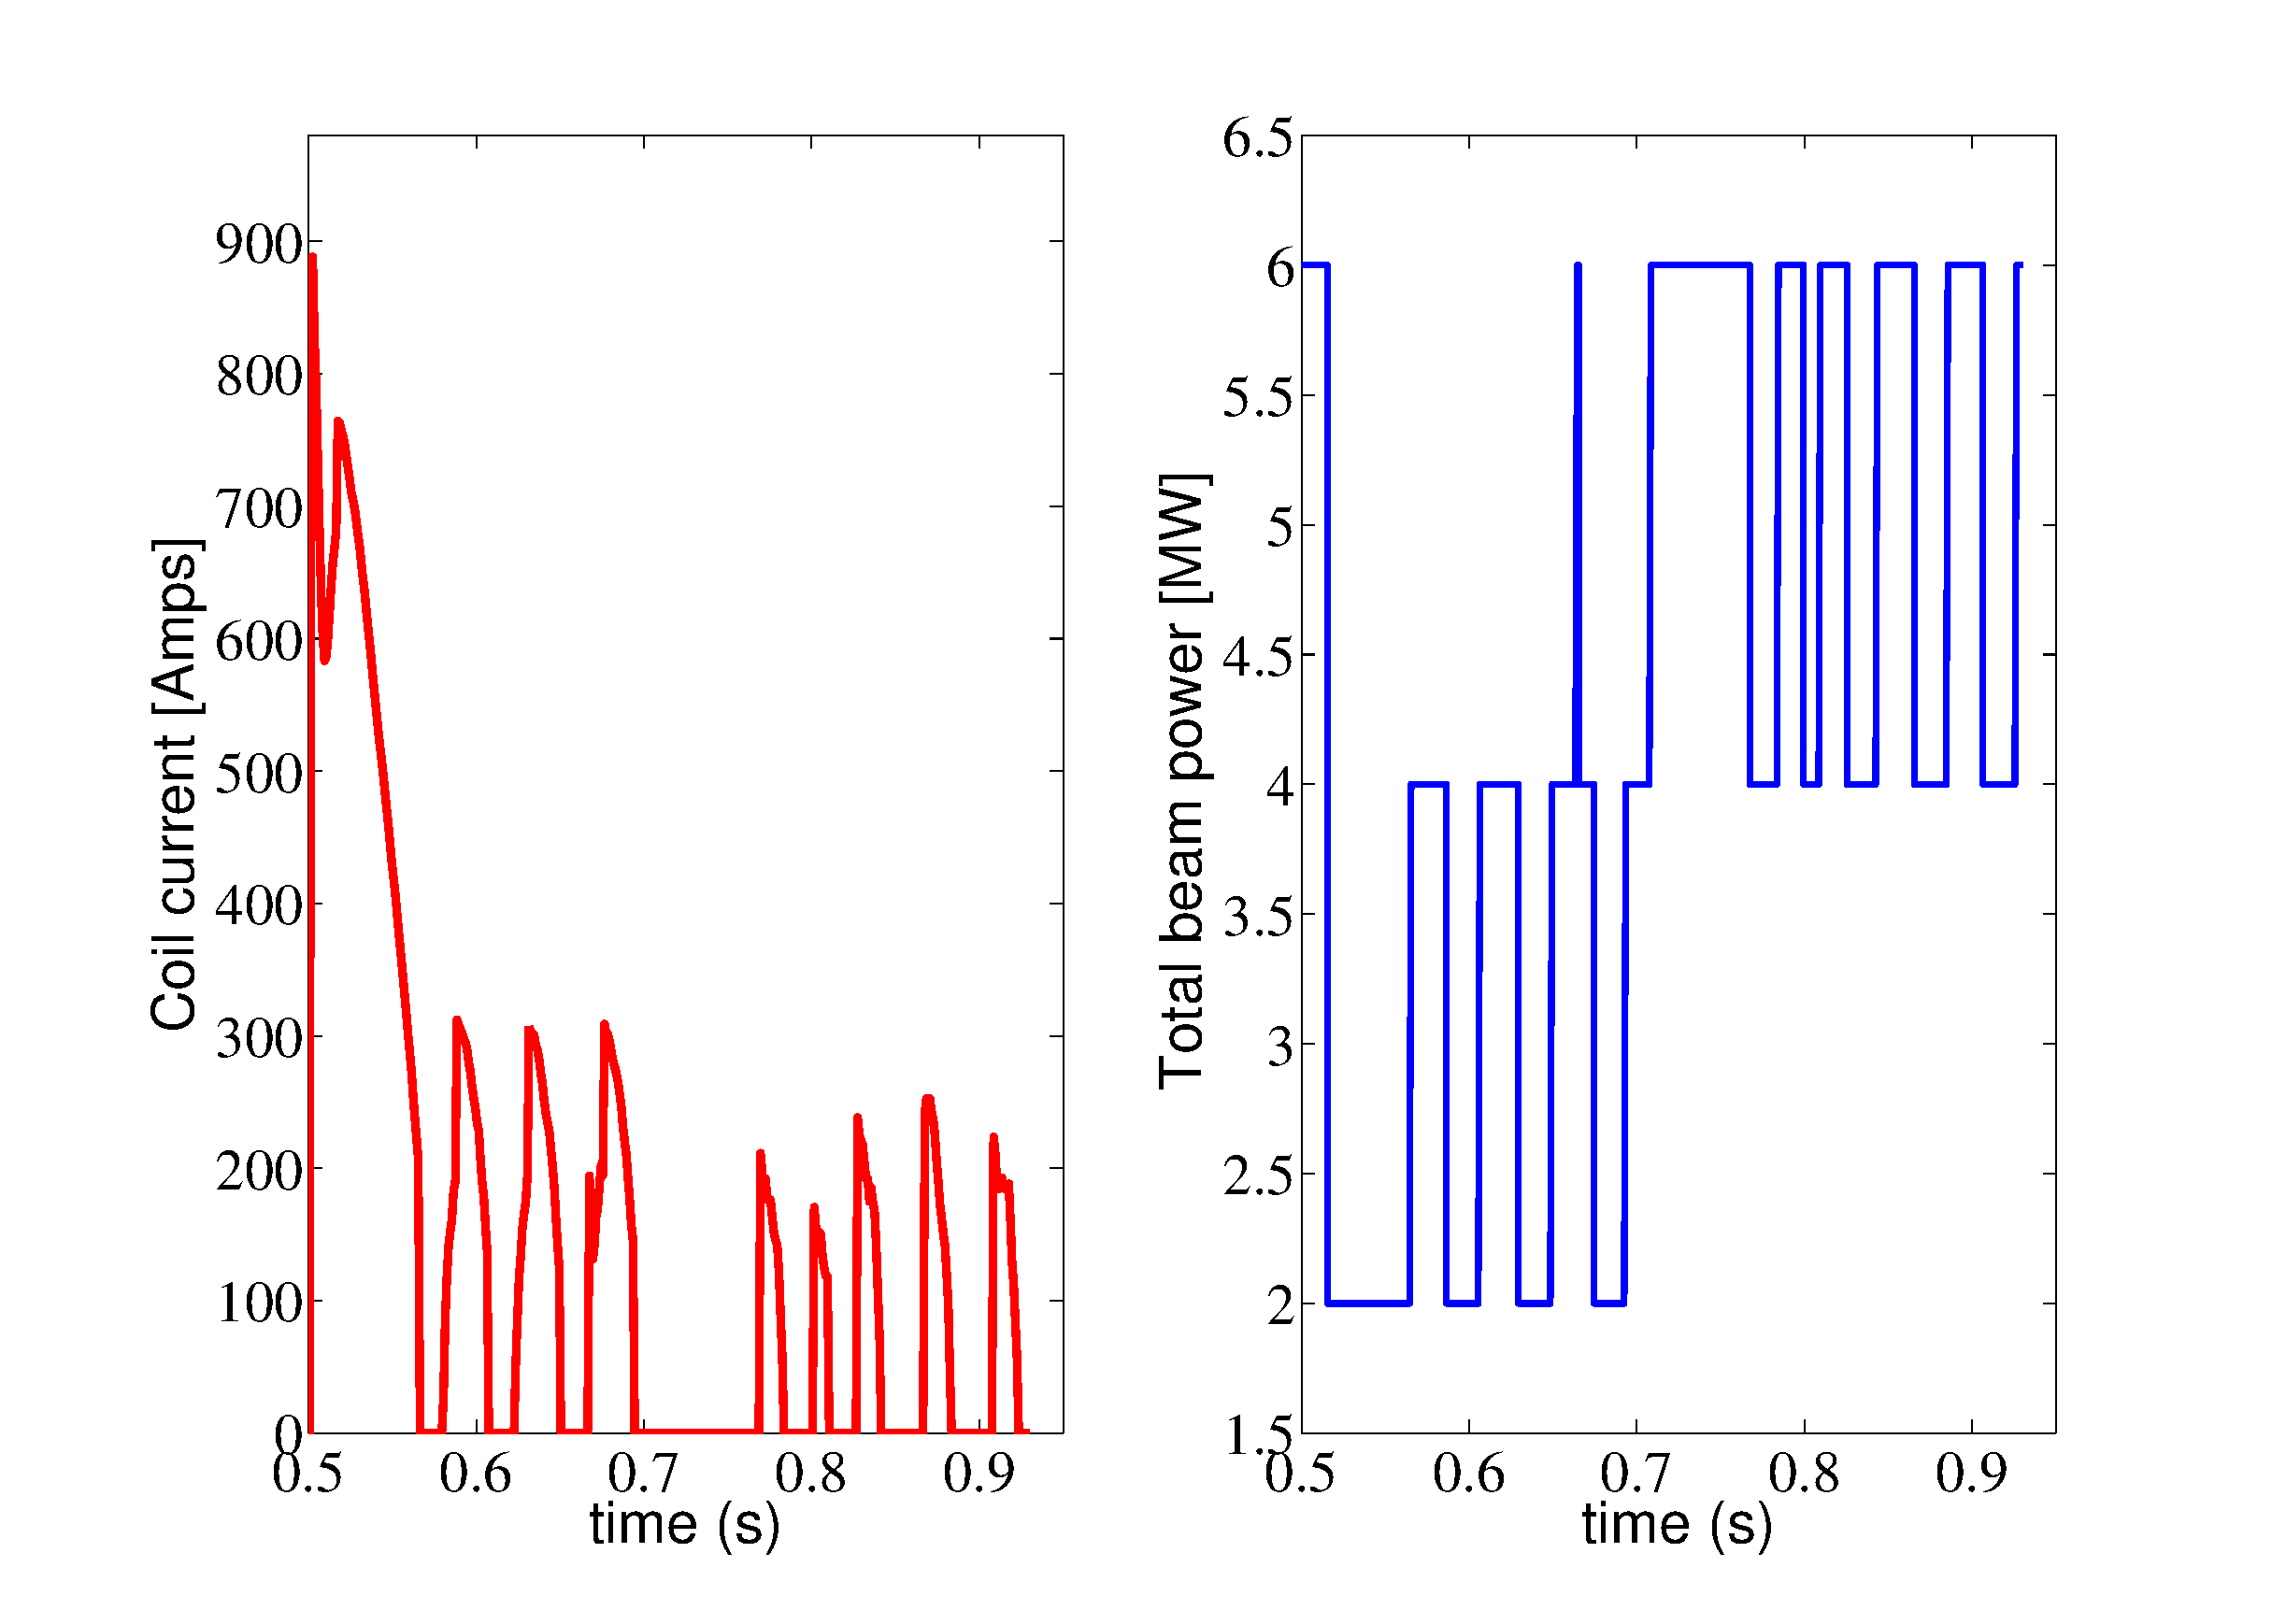
\includegraphics[width=\linewidth]{imene_figs/Goum15ln}
\caption{Time evolution of the coil current and the overall beams power (cycle time $0.015  s$). }
\label{fig:rot15}
\end{figure}

Figure~\ref{fig:rot14} compares the rotation measurements when the PWM controller is applied to both the reduced-order model and the TRANSP predictive model in order to reach two targets.
Before $t=0.5$\,s, both models are not controlled (open loop), the measurements are already shown to be the steady-state values shown in Figure~\ref{Goum12}.
At $t = 0.5$\,s, the controller is turned on (closed loop), and the goal is to reach the first target profile measurement points defined by the two red dots in Figure~\ref{fig:rot11}. At $t = 0.7$\,s, the  target profile changes to the second one which is defined by the two blue dots in Figure~\ref{fig:rot11}.
The green line represents the reduced-order model outputs, the blue line represents the TRANSP model. The oscillations are due to the modulations that occurs on each of the beam power source. The total beam power is represented in Figure~\ref{fig:rot15} (right). The coil current in this case (Figure~\ref{fig:rot15} left) changes to compensate for when the beam power is too high in order to decrease the toroidal rotation and thus limit the rotation overshoot.
In this example, the duty cycle duration is 15\,ms which gives a reasonable amplitude of oscillation while reaching both targets within the momentum diffusion time ($0.1 s$).

Figure~\ref{fig:rot16} and Figure~\ref{fig:rot17} represent the same quantities as in Figure~\ref{fig:rot14} and Figure~\ref{fig:rot15} respectively, but for a different duty cycle duration (6\,ms) which is smaller that the the 10\,ms refractory period.
The resulting rotation measurements are more oscillatory but the amplitude is better damped. The trade off is that we have to activate the controller more often and thus formulate more requests to the real device.

The reduced-order model in both cases is very close to the TRANSP which again shows that the simplified model gives us a good qualitative approximation of the TRANSP rotation prediction model.

\begin{figure}
\centering
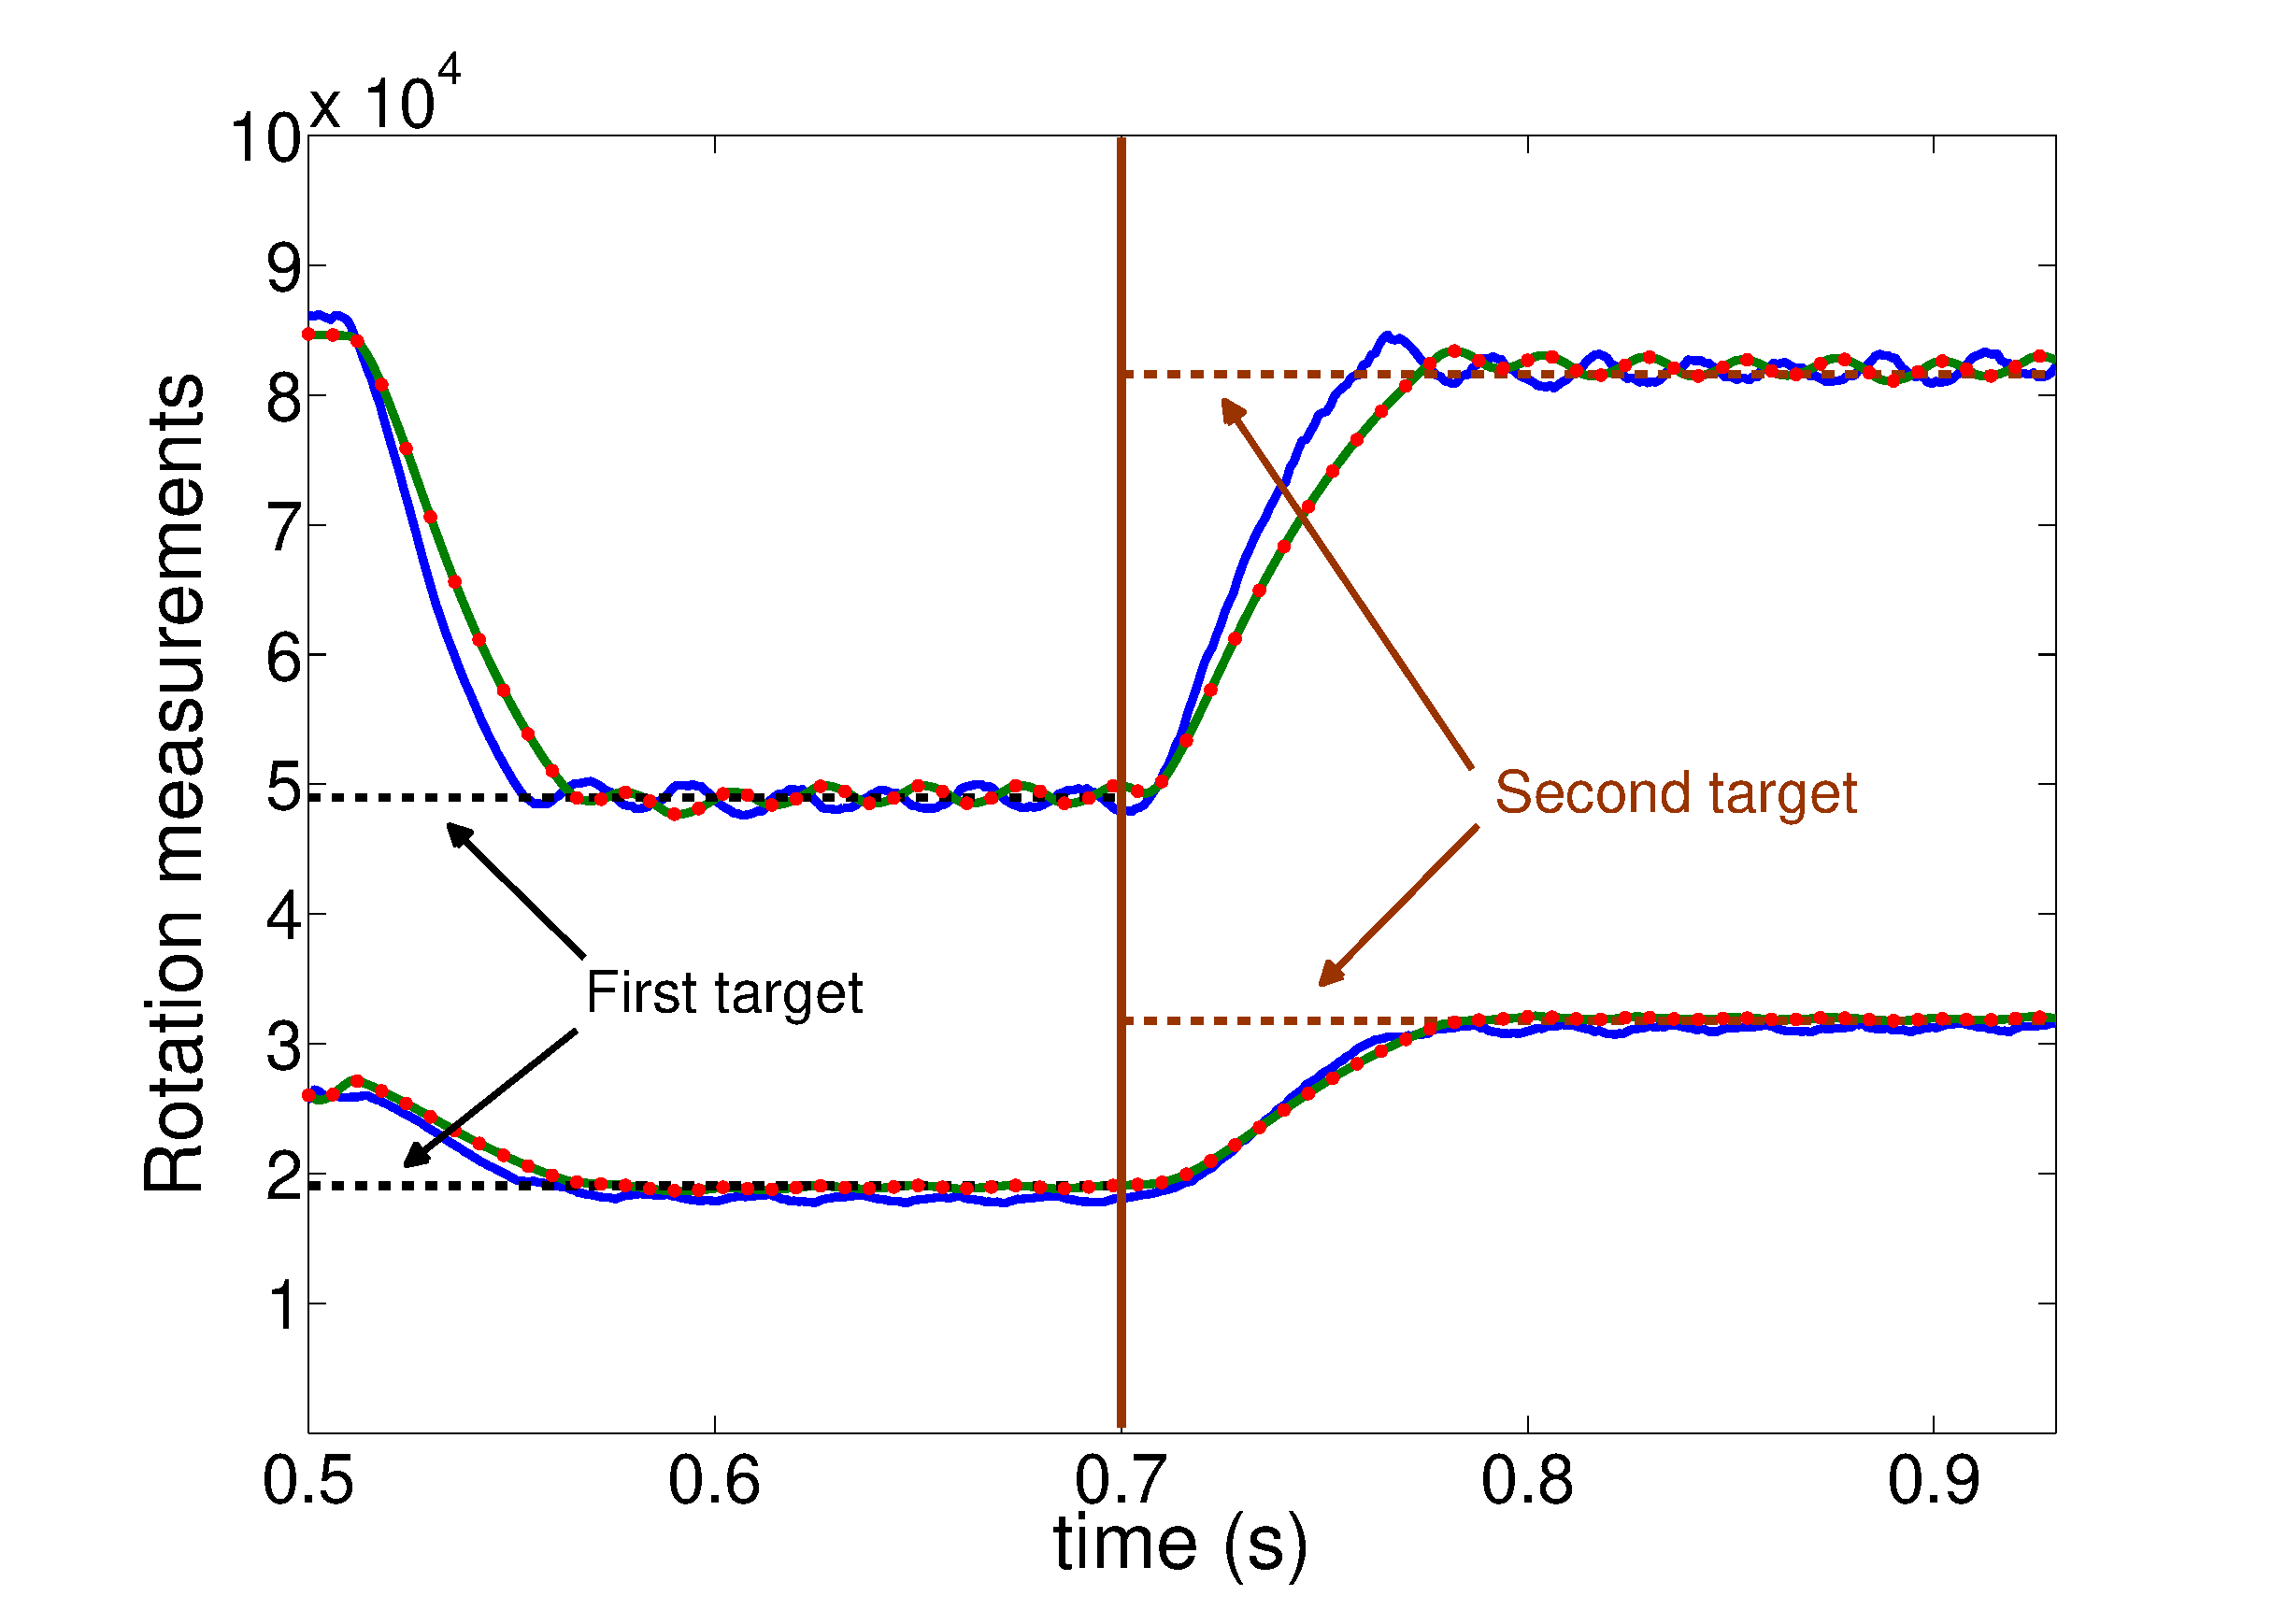
\includegraphics[width=\linewidth]{imene_figs/Goum16ln}
\caption{Comparison of the rotation measurements when PWM applied for both the reduced-order model (green lines) and the TRANSP predictive model (blue lines). The red dots represents the cycle times (every $0.006 s$).}
\label{fig:rot16}
\end{figure}

\begin{figure}
\centering
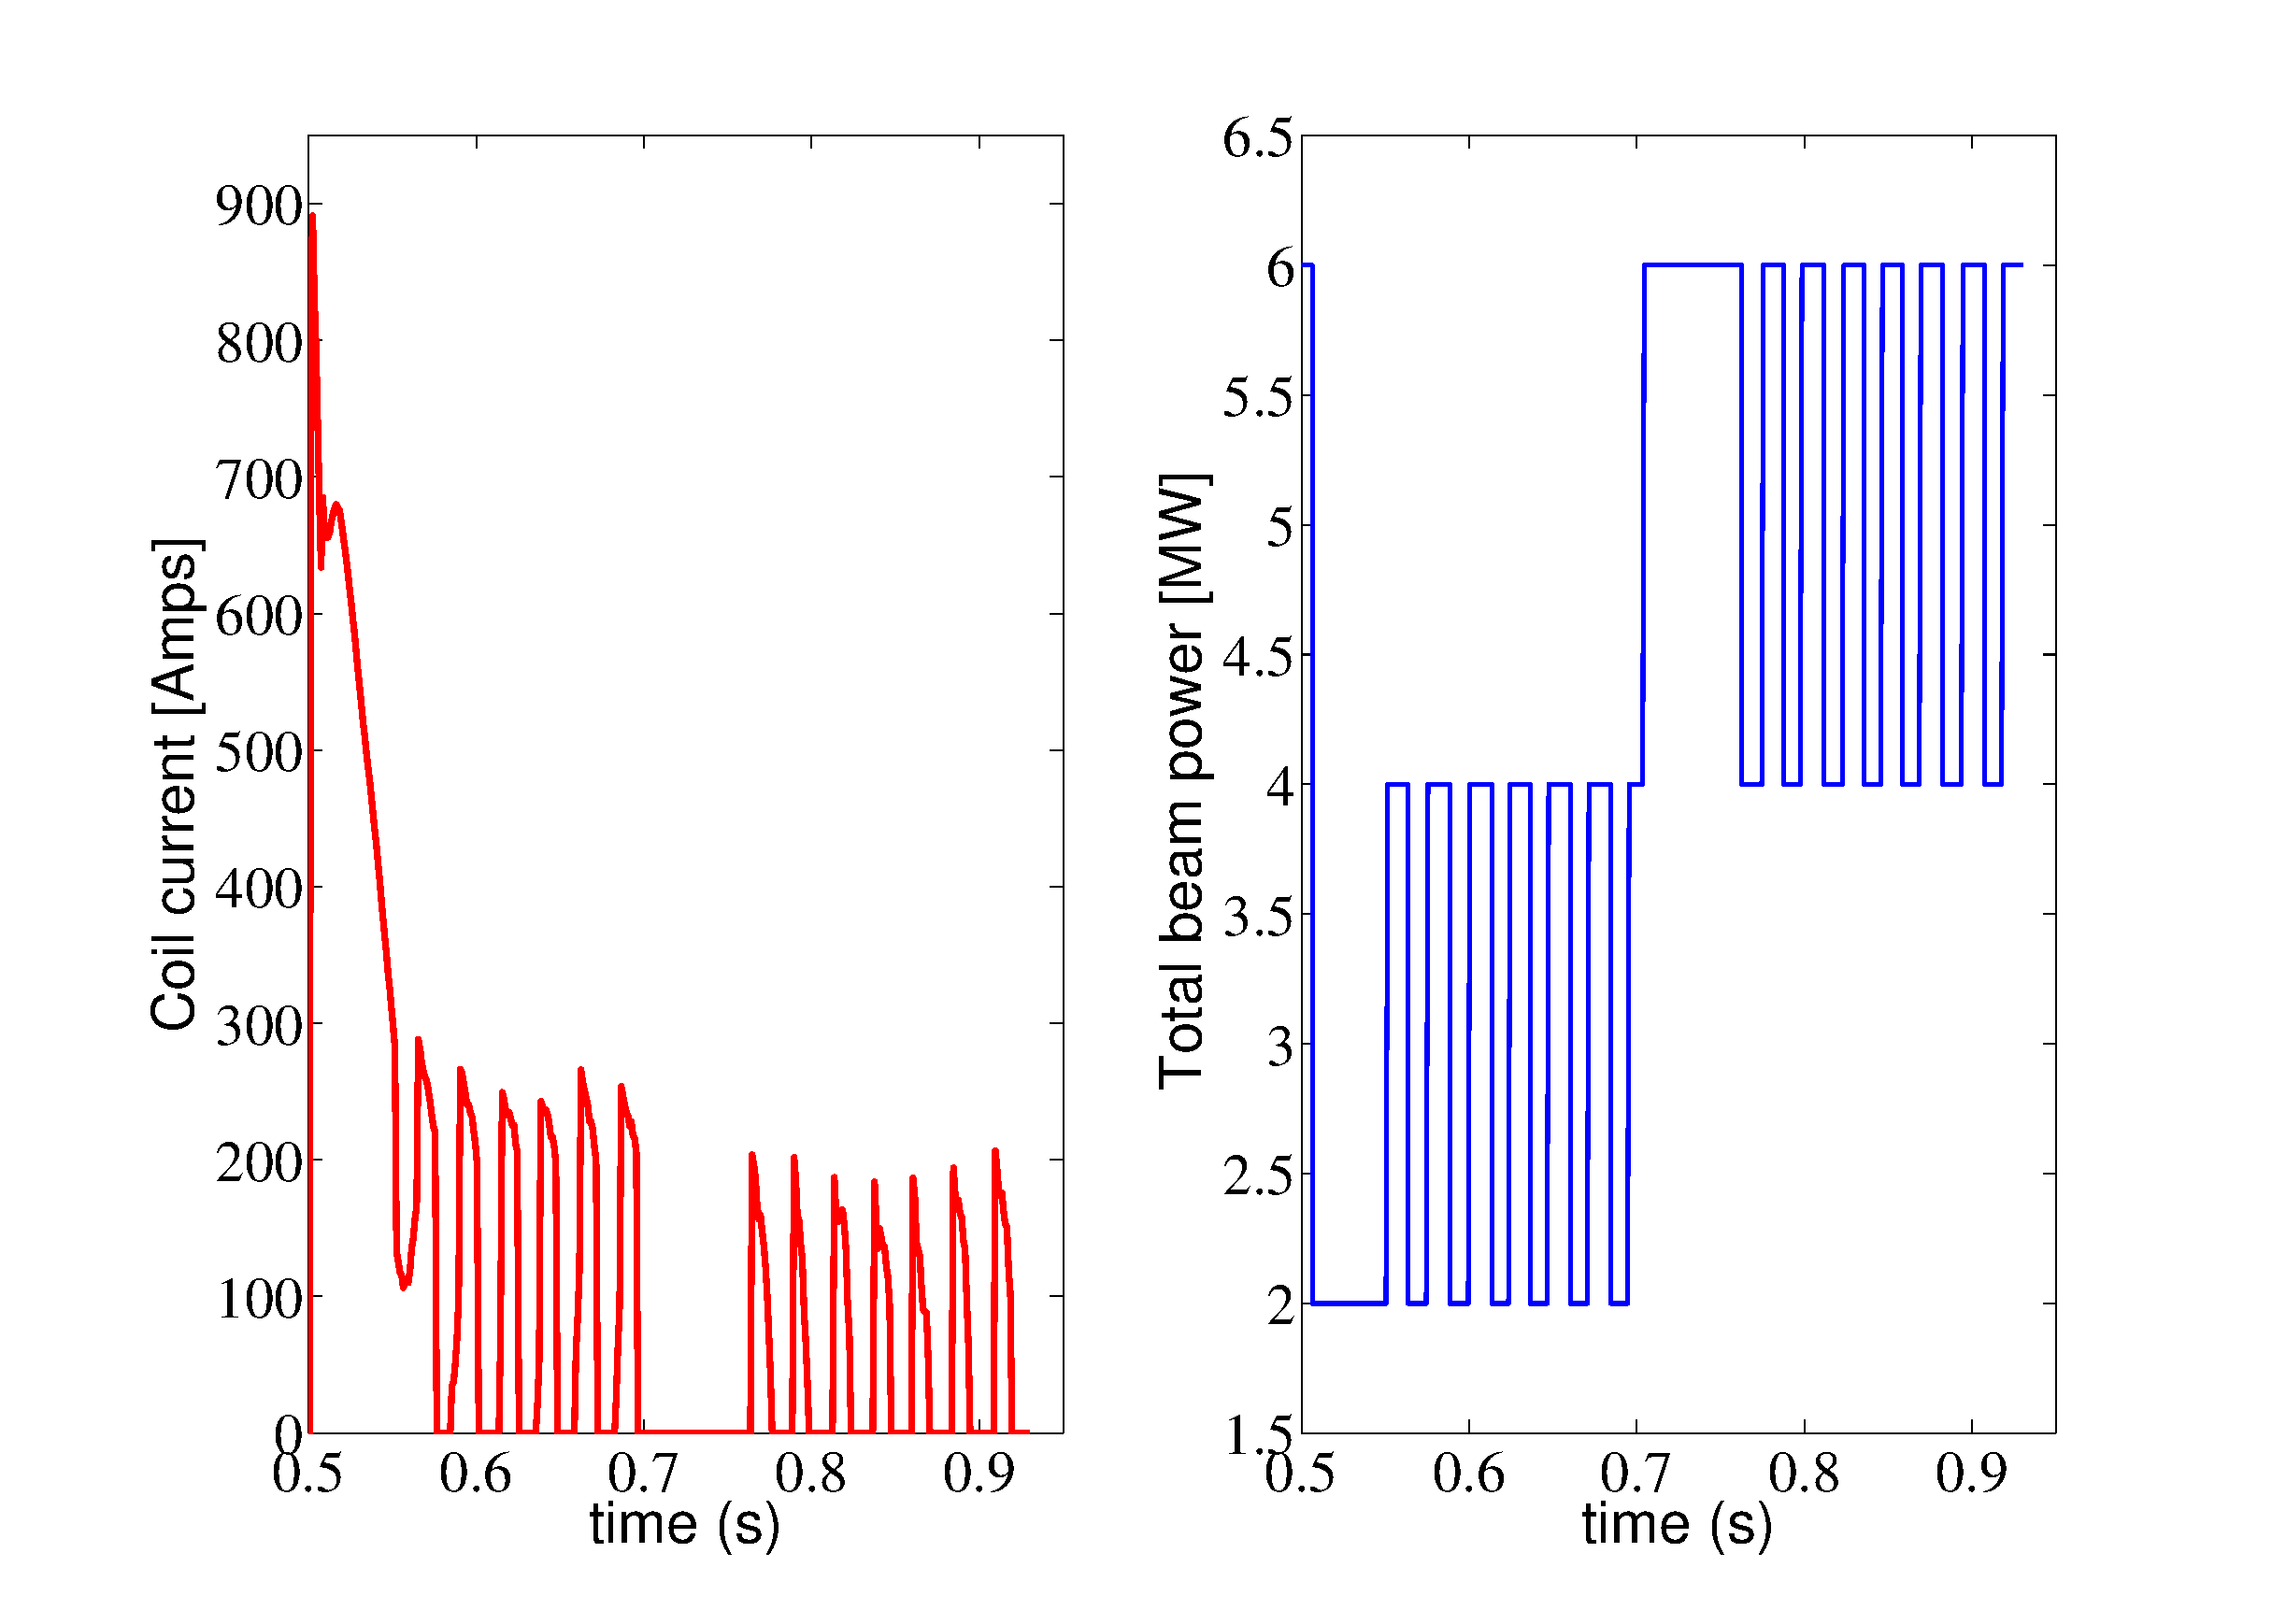
\includegraphics[width=\linewidth]{imene_figs/Goum17ln}
\caption{Time evolution of the coil current and the overall beams power (cycle time $0.006 s$). }
\label{fig:rot17}
\end{figure}


\section{Summary and conclusions}
The main motivation of this work is model-based control of plasma rotation in tokamaks.
In the above plasma control demonstrations, a simple reduced order model has been built to capture the rotational toroidal momentum balance, applied specifically to the NSTX device. The neutral beam injection and the neoclassical toroidal viscosity are considered in this model as actuators. The output from the present model have been compared with analysis from a predictive model of NSTX and were found to be in good agreement.
Based on this simplified model, a complete feedback control design using optimal control techniques as shown above and enables controlling the plasma about a desired profile. This reduced-order controller was then tested using the NSTX predictive model and enabled the rotation profile to reach the desired profile.

Generally, broader toroidal rotation profile brings more stability to the plasma \cite{Sabbagh10} and local rotation shear can affect MHD modes  \cite{Gerhardt09}. In the new upgrade of the device, NSTX-U,three  additional NBI sources (Figure~{\ref{NBI_pics}}) will provide significantly different torque profiles which can affect a broader region of the plasma, specifically towards the edge and can change the shear locally. In this case, the controller can use these added beam sources allowing significantly greater control of plasma instabilities.
Furthermore, while only the n = 3 applied field configuration was considered for the NTV actuator, it is possible to include different applied field spectra which can change the NTV torque profile. For example, an $n=1$ field configuration can allow a deeper penetration of this torque profile which will expand the capability of rotation control.

The present controller was designed using models tuned to match experimental data. A next step could be to develop control-oriented models directly from simulations. This capability would have a large impact: fewer experiments would be needed to calibrate the models/controllers, and more importantly, one could predict actuator requirements (e.g., amplitude, bandwidth, latency), and any inherent performance limitations for future machines such as ITER.
These control-oriented models such as those being developed in TRANSP for NSTX-Upgrade will be tested for their robustness in producing greater range of target profile shapes in order to maintain and optimize plasma stability for the worst case scenarios. 

 
\ack 

This work was supported by the U.S. Department of Energy under contract No. DE-AC02-09CH11466 (PPPL) and U.S. Department of Energy  grant number DE-FG02-99ER54524 (Columbia University). 
\section*{References}

\bibliographystyle{unsrt}
\bibliography{pap14}


\end{document}

